\section{Vehicle Design and Development}
  Finalisation of the chosen concepts for the development of the rover meant that the project could progress to the detailed design stages. It was discussed in Section~\ref{subsubsec:central-control-system} that the mechanical design of the vehicle would be driving of the overall design, specifically the software aspects, and thus the report will deal with the mechanical and electronic detailed design first.
  
  \subsection{Mechanical Design}
    The mechanical design was initiated by planning the basic layout of mechanical subsystems and components and from that point developing each system further. In this section, the choice of scale (and hence dimensions) is followed by the overall plan of the mechanical layout. Subsystems that are peripheral to the body structure are then covered. These include the suspension, differential and mast subsystems. Finally, the design of the body structure is described as well as detail surrounding the model as a whole.
    
    \subsubsection{Scale and Dimensions}
      Replication of \textit{Curiosity} on an aesthetic level was a project aim to increase the viewers' and users' sense of familiarity with the real \textit{Curiosity} rover, a way of promoting a more engaging experience. The replication process identified that proportion was an effective and achievable starting point and it was decided that as many of the parts as possible be based off the dimensions of the corresponding part on \textit{Curiosity}, brought down to scale by a predetermined factor. Scale was constrained primarily by the cost and manufacturing time of parts that were required to be 3D printed; the larger the model, the greater the amount of material required and the longer it would take to print it. The print bed size was also a constraint in this regard. More details pertaining to the use of 3D printing facilities can be found in Section~\ref{subsubsec:additive-manufacture}.
      
      \begin{figure}[h]
        \centering
        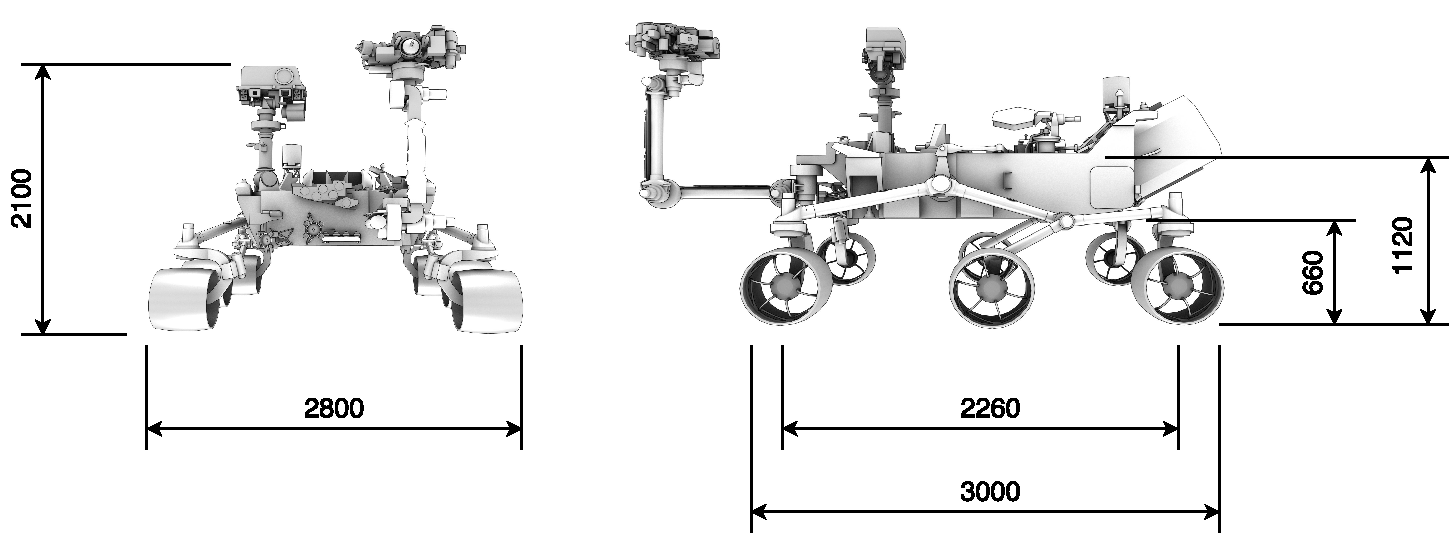
\includegraphics[width=0.9\linewidth]{figures/mechDesign-curiosityDimensions}
        \caption[Diagram indicating the external dimensions of \textit{Curiosity}, in millimetres, these references provided]{Diagram indicating the external dimensions of \textit{Curiosity}, in millimetres, these references provided \cite{nasa3D}}
        \label{fig:mechdesign-curiosityDimensions}
      \end{figure}
      
      The dimensions shown in Figure~\ref{fig:mechdesign-curiosityDimensions} were retrieved from \cite{nasajulypresskit} and \cite{roverThermal_2016} as guidelines. External dimensions only and no other dimensions were available that might have provided a more detailed insight into each of the subsystems and components. A 3D model of a small scale, static, printable model of \textit{Curiosity} published by NASA was found and used for extraction of the 3D proportions of the individual components \cite{nasa3Dprint}. While this model was not ideal in terms of representative accuracy, it provided the much needed basis on which to generate the designs of parts with an acceptable level of similarity. From these details, it was decided that the rover be built at a 1:10 scale, making the total length and width of the model, including the wheels, 300 mm and 280 mm respectively. This scale took into account allowing the model enough space to be used within the typical exhibit size outlined in the problem definition as well as 3D printing capabilities. The scale ensured that anticipated electronic components would fit into the body structure and that mounting of bearings and the chosen standard size of servo motors was reasonable.
      
      The chosen scale gave rise to a set of external dimensions for each of the subsystems, highlighted in Table~\ref{tab:design-referenceDimensions}. The guideline full-scale dimensions in Figure~\ref{fig:mechdesign-curiosityDimensions} were used against the 3D model in \cite{nasa3Dprint}, here-onwards referred to as the reference model, to derive the scale of this reference. This scale was then used to obtain external, high-level dimensions for all of the subsystems and components ensuring that they remained in proportion. In some instances, it was not possible to adhere strictly to the scaling and/or placement of certain components. Such exceptions are discussed in their respective sections.
            
      The reference model, which was in Standard Tessellation Language (STL) format, was imported into a CAD package with millimetre units and evaluated in that state to result in a scale of 1:1.7037 (reference model as to \textit{Curiosity}). The dimensions shown in Table~\ref{tab:design-referenceDimensions} are of priority components and subsystems only, omitting details related to components that were intended to serve aesthetic purposes only (such as a mock-up of the RTG).
      
      \begin{table}[h!]
      \centering
      \begin{tabular}{@{}cccc@{}}
      \toprule
      \textbf{Feature}            & \textbf{Dimension}            & \textbf{Code} & \textbf{Value (mm)} \\ \midrule
      \multirow{3}{*}{Rover}      & Height                        & A1   & 210   \\
                                  & Width                         & A2   & 280   \\
                                  & Depth                         & A3   & 300   \\ \midrule
      \multirow{4}{*}{Body}       & Height                        & B1   & 46    \\
                                  & Width                         & B2   & 136   \\
                                  & Depth                         & B3   & 190   \\
                                  & Ground Clearance              & B4   & 66    \\ \midrule
      \multirow{5}{*}{Suspension} & Height                        & C1   & 122   \\
                                  & Width                         & C2   & 72    \\
                                  & Depth                         & C3   & 271   \\
                                  & Wheel Pitch                   & C4   & 119   \\
                                  & Center-pivot to Body Front    & C5   & 71    \\ \midrule
      \multirow{2}{*}{Wheel}      & Diameter                      & D1   & 50    \\
                                  & Depth                         & D2   & 40    \\ \midrule
      \multirow{5}{*}{Mast}       & Height                        & E1   & 98    \\
                                  & Width                         & E2   & 62    \\
                                  & Depth                         & E3   & 50    \\
                                  & Position from font deck edge  & E4   & 28    \\
                                  & Position from right deck edge & E5   & 28    \\ \midrule
      \multirow{3}{*}{Head}       & Height                        & F1   & 30    \\
                                  & Width                         & F2   & 60    \\
                                  & Depth                         & F3   & 50    \\ \bottomrule
      \end{tabular}
      \caption{Table showing the external dimensions of components and subsystems obtained from the reference model \cite{nasa3Dprint}}
      \label{tab:design-referenceDimensions}
      \end{table}
      
    \subsubsection{Layout Plan}
      The dimensions in Table~\ref{tab:design-referenceDimensions} were used to construct a plan of the layout of subsystems to be used for further detailed design. The plan can be seen in Figure~\ref{fig:mechDesign-layoutPlan}, along with selected dimensions from the Table.
      
      \begin{figure}[h!]
        \centering
        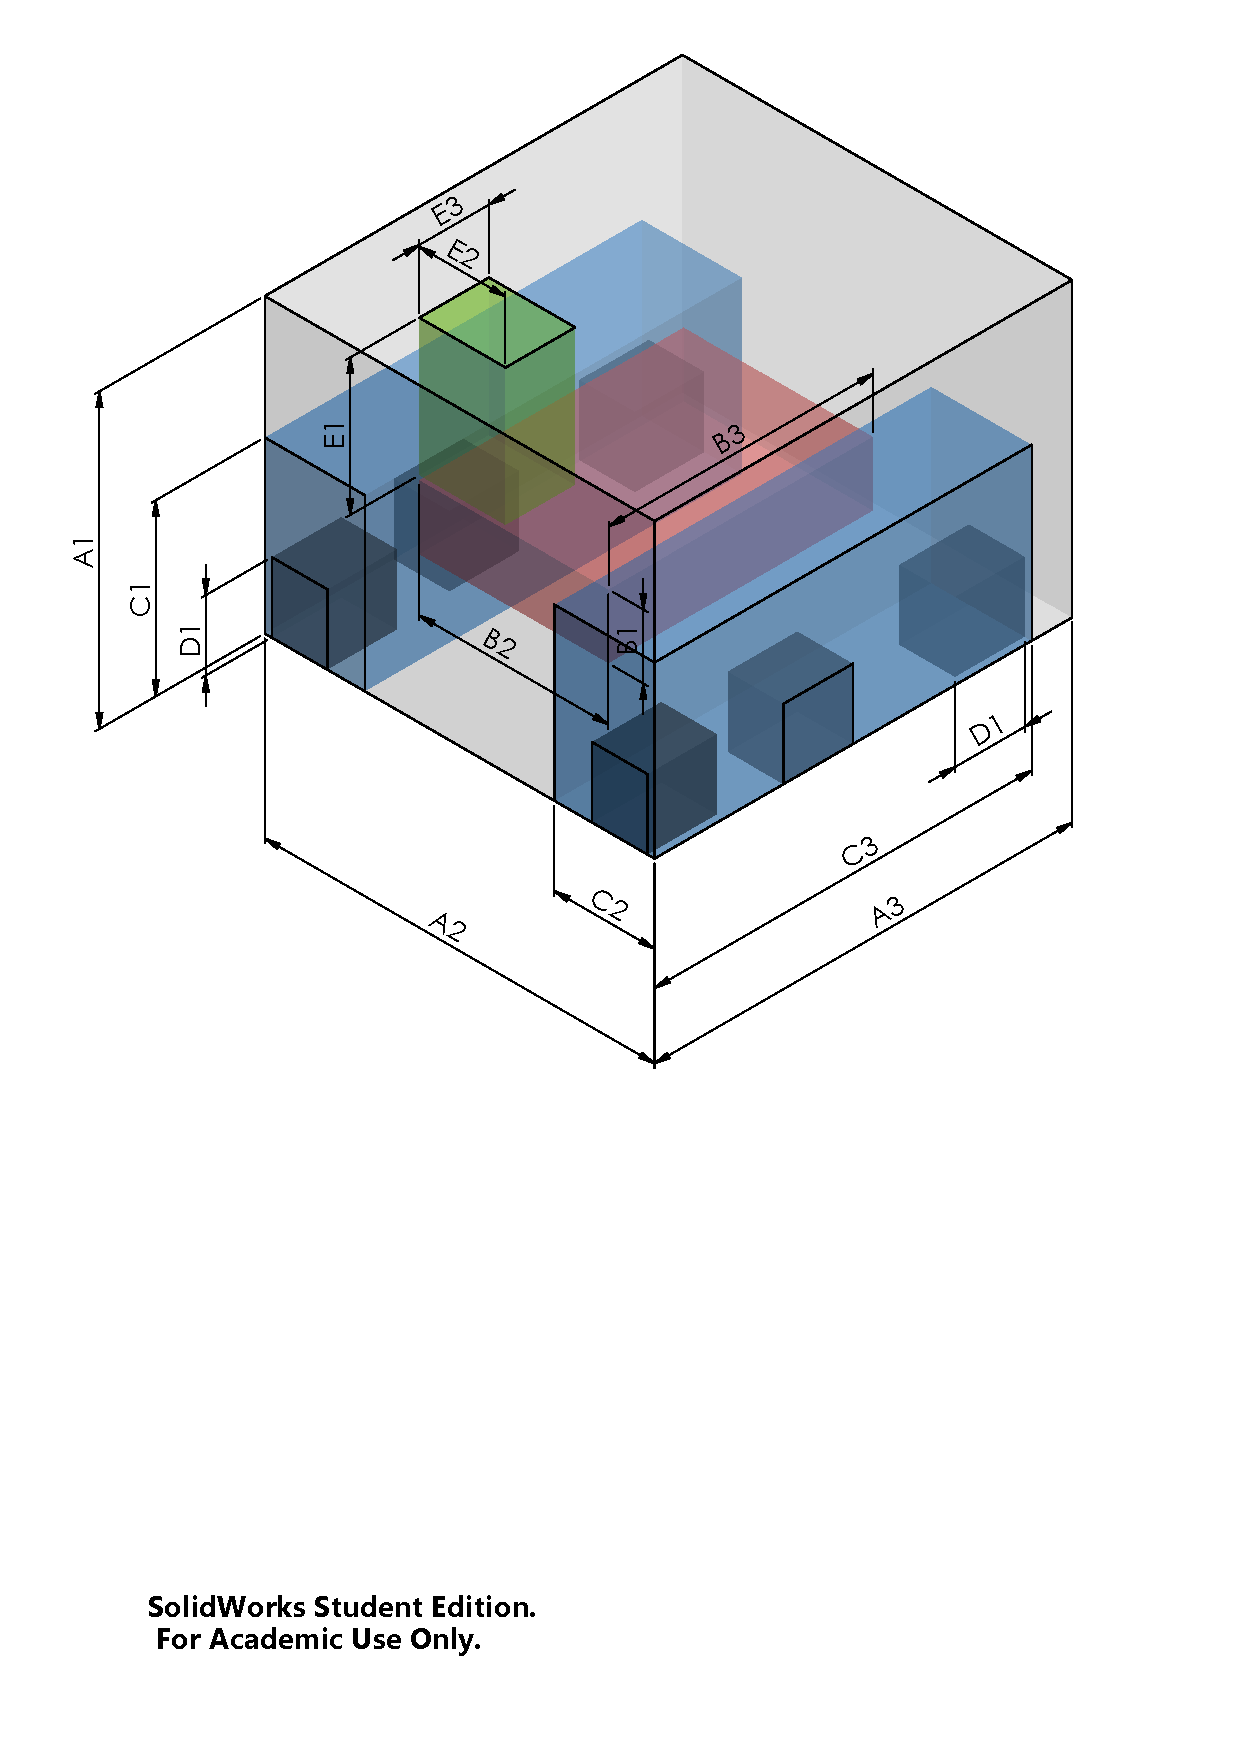
\includegraphics[clip, trim=1cm 11cm 1cm 0cm, width=0.9\linewidth]{figures/mechDesign-layoutPlan}
        \caption[Isometric view of the 3D layout plan of the rover with a subset of the external dimensions shown]{Isometric view of the 3D layout plan of the rover with a subset of the external dimensions shown}
        \label{fig:mechDesign-layoutPlan}
      \end{figure}

      
    \subsubsection{Standard Features}
      Prior to designing and developing the components and parts in detail, standard feature dimensions and sizes were set up to maintain a level of consistency throughout the process. This included features such as holes, walls and fasteners and served as a general guideline allowing for variation of these parameters, if required. Table~\ref{tab:featureStandards} highlights these feature details.
      
      \begin{table}[h!]
      \centering
      \begin{tabular}{@{}llL{0.6\textwidth}@{}}
      \toprule
      \textbf{Feature} & \textbf{Size} & \textbf{Comments} \\ \midrule
      Fasteners & M2 - M3 & Full pan-slotted screw, hex nut and flat washer stack. M3 as first priority dropped down to M2 if the part dimensions or circumstances do not allow. \\ \midrule
      Holes & M2 - M3 & Holes were to match the fasteners in terms of size. \\ \midrule
      Hole Clearances & 0.5 mm & Clearance made to be over a standard fit clearance in anticipation of spread of the surfaces of the part during the 3D printing process. \\ \midrule
      Wall Thicknesses & \begin{tabular}[c]{@{}l@{}}Major: 5mm\\ Minor: 3mm\end{tabular} & Major walls used where significant structural integrity required, whereas minor walls were used both for less significant areas or areas where available space is a constraint \\ \bottomrule
      \end{tabular}
      \caption{Table indicating standards for common features across the entire design}
      \label{tab:featureStandards}
      \end{table}
      
    \subsubsection{Suspension}
      The collection of joints, pivots, struts and wheels was collectively referred to as the suspension system, one positioned on either side of the body structure. Each side of the suspension system included two fixed link mechanisms, the ``rocker'' and the ``bogie'' as part of the ``rocker-bogie'' principle as highlighted in Section~\ref{subsubsec:lit-manoeuvrability}. During the conceptual design phase, it was decided that this mechanism be constructed by connecting aluminium tube pieces to 3D printed joints, on the ends of which the pivots and struts could be attached for the wheels.
      
      The design started with the identification of the components required and a map of how they would be fitted together which included the names of each part for identification throughout the process. Figure~\ref{fig:mechdesign-suspensionLinkageMap} shows this mapping, which can be considered as a lower-level conceptual plan of the system.
      
      \begin{figure}[h!]
        \centering
        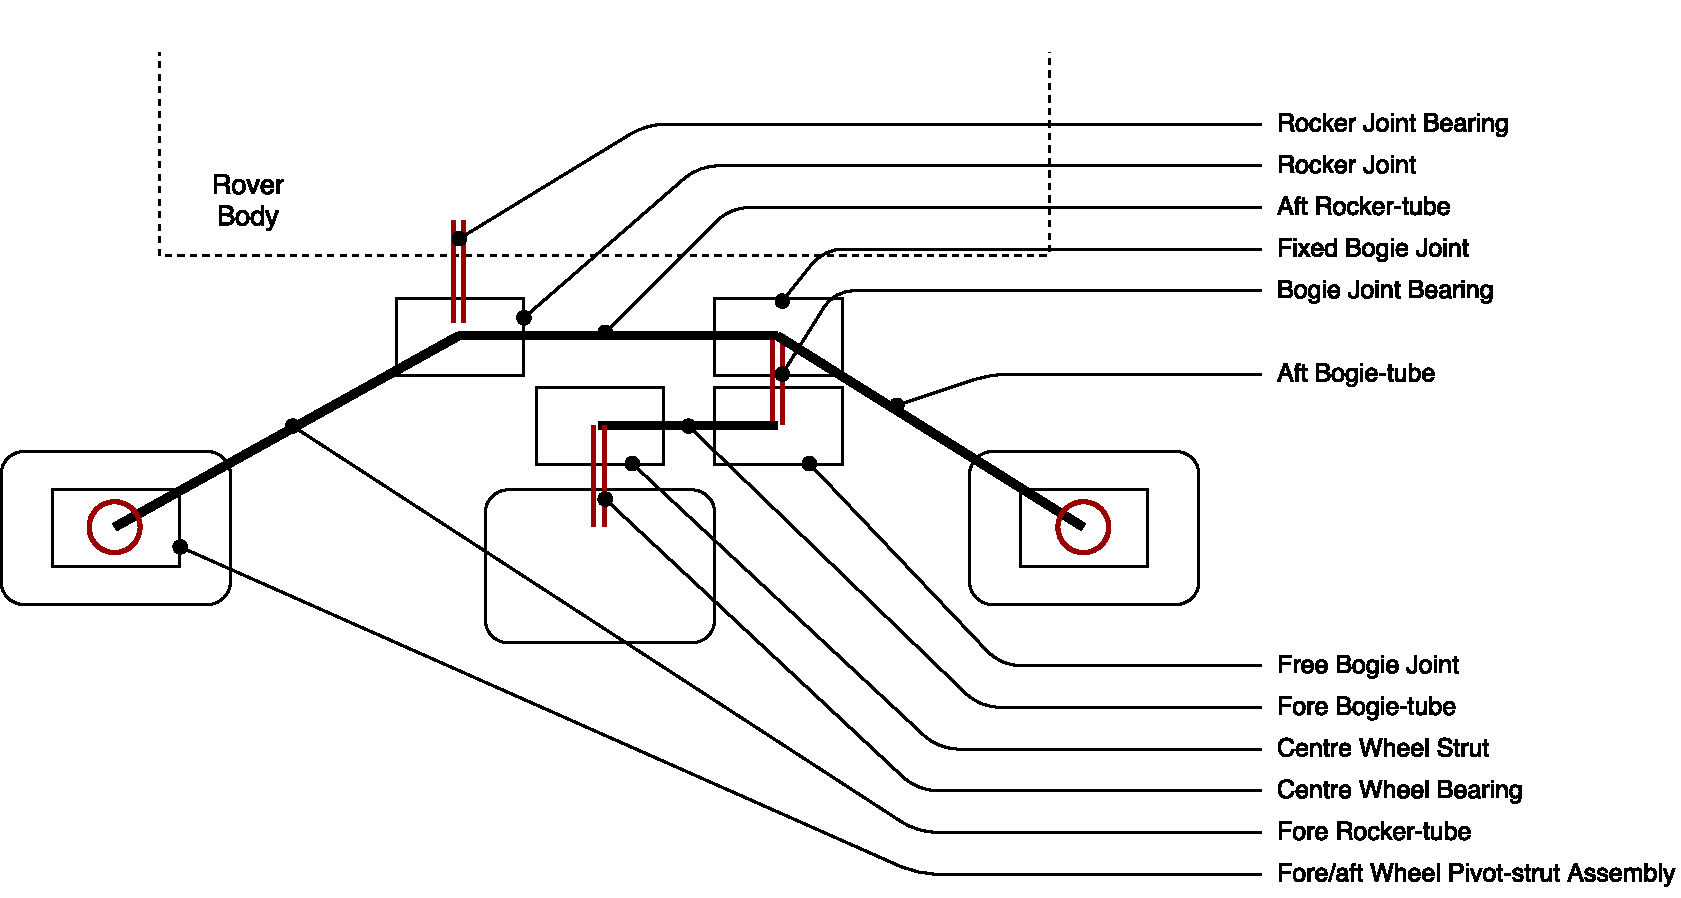
\includegraphics[width=1\linewidth]{figures/mechDesign-suspensionLinkageMap}
        \caption[Schematic diagram of a top view of the suspension system]{Schematic diagram of a top view of the suspension system}
        \label{fig:mechdesign-suspensionLinkageMap}
      \end{figure}
      
      It was noted that the ratios of the tubing or beams on \textit{Curiosity} (and rocker-bogie mechanisms in general) are important since they determine the system's range of motion, affecting the rover's ability to traverse the terrain. The reference model in \cite{nasa3Dprint} was not able to provide this kind of detail, and so the angles and positions of the centre-points of joints and axes of pivots and wheels had to be constructed from reference images of the rover. What was known was the distance of the wheels away from the side of the rover body, that the pivot centre-points were directly above the centres of the wheels and that the aft rocker-tube and the fore bogie-tube were parallel to the body of the rover in the $x$-$y$ plane. Figure \ref{fig:mechDesign-suspensionReferences} includes the images that were used to find these details.
      
      \begin{figure}[h!]
      \centering
      \subfloat[]{
        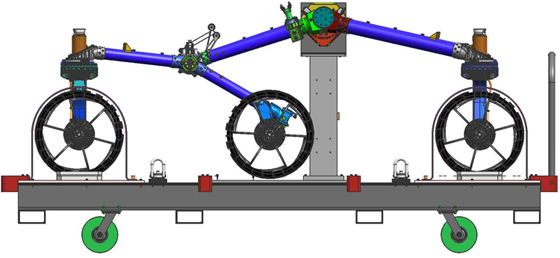
\includegraphics[width=.45\linewidth]{figures/mechDesign-suspensionReference1.jpg}
      }
      \qquad
      \subfloat[]{
        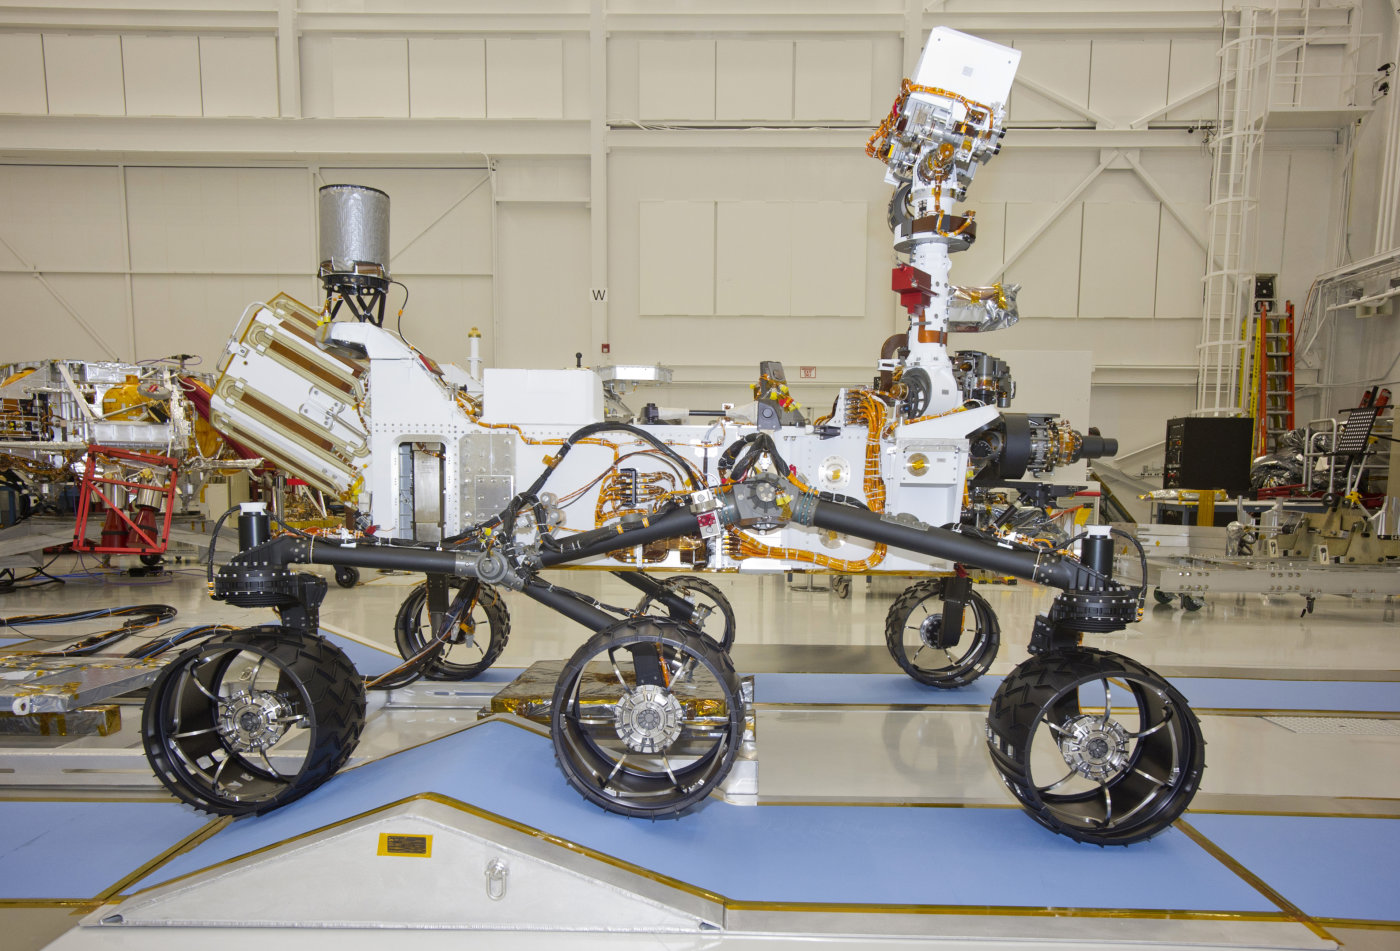
\includegraphics[width=.45\linewidth]{figures/mechDesign-suspensionReference2.jpg}
      }
      \caption[The two images used for obtaining the positions of joints and pivots of the suspension system in 3D space]{The two images used for obtaining the positions of joints and pivots of the suspension system in 3D space. \cite{fig:mechDesign-suspensionReferences1_cite} and \cite{fig:mechDesign-suspensionReferences2_cite}, respectively.}
      \label{fig:mechDesign-suspensionReferences}
      \end{figure}

      A skeleton layout generated from the positional data obtained is shown in Figure~\ref{fig:mechDesign-suspension3d} where a 2D sketch was created as a starting point from which a 3D sketch of the layout was formed. The skeleton sketch was rigid in the position whereby all three wheels were at rest on a flat, horizontal surface parallel to the rover body.
            
      \begin{figure}[h!]
        \centering
        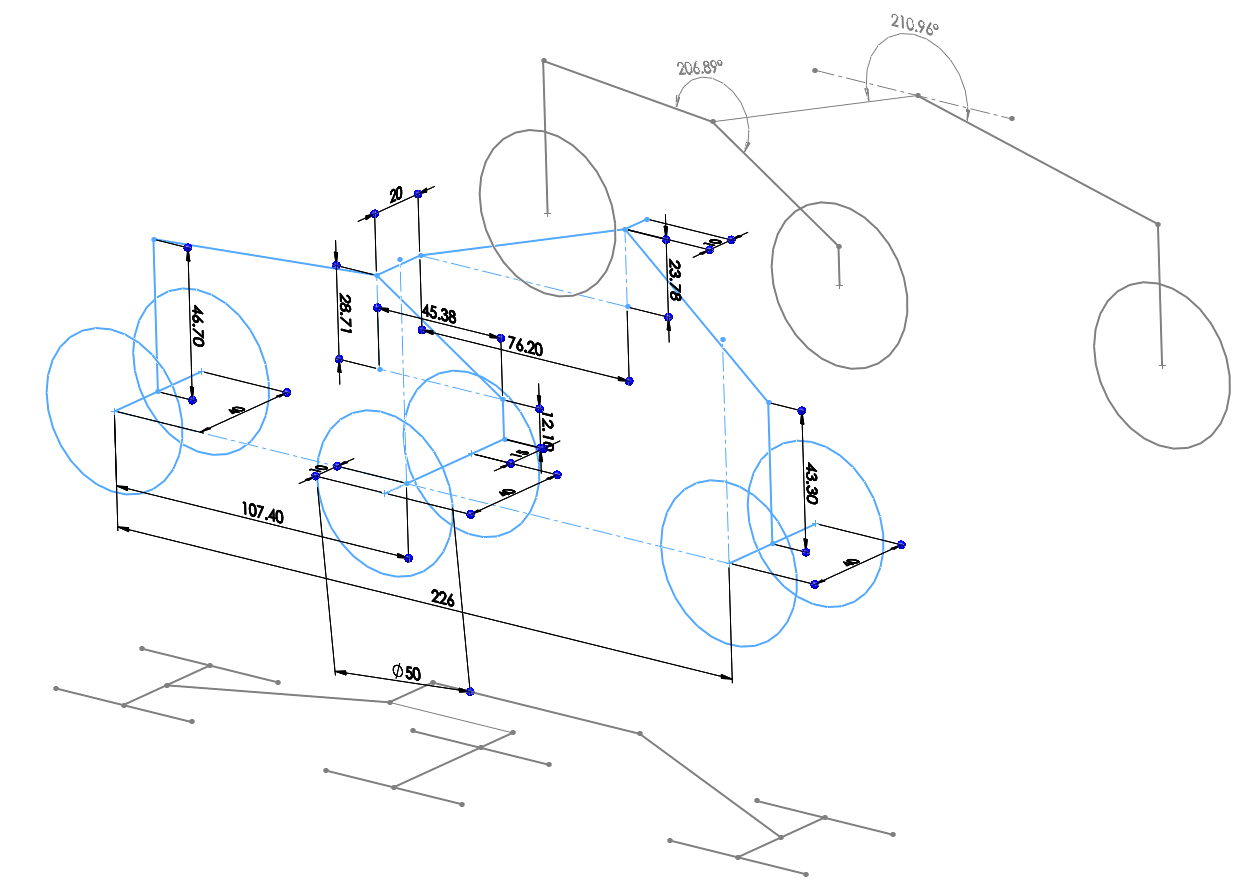
\includegraphics[width=0.9\linewidth]{figures/suspension3D}
        \caption[Isometric view of the 3D sketch of the generated suspension system skeleton used for positioning of designed parts]{Isometric view of the 3D sketch of the generated suspension system skeleton used for positioning of designed parts}
        \label{fig:mechDesign-suspension3d}
      \end{figure}
      
      The joints, pivots and struts were then developed around the axes and centre-points in the sketch, a work-flow typical of the CAD package used.
      
      \subheading{Joints}\\\\
        One side of the suspension system required three different joints: the rocker joint and fixed and free bogie joints. The bogie joints were the simpler of the three and provided a means for the bogie to pivot about one of the ends of the rocker. The fixed joint was fixed in rotation on the end of the rocker while the free joint rotated about a point on the free joint. The rocker joint allows for the entire mechanism to pivot about a point on the side of the rover body as well as allowing attachment of the differential bar in order to keep the two sides of the suspension system coordinated.
        
        It was decided that the rotation of the joints be aided by use of bearings mounted on aluminium shafts. The aluminium would not add excessive amounts of weight to the system but still provide the rigidity required between the joints. Bearings were then required to be fixed into the rocker and free bogie joints with a shaft extending from the side of the body for the rocker joint bearings and another shaft mounted in the fixed bogie joint. Various methods of mounting bearings and shafts into 3D printed parts were considered, however, the most commonly employed technique involved press-fitting both types of components. At this point it was clear that printing the parts from a material which allowed for a certain amount of flexibility (i.e. less brittleness) would suit press-fitting bearings and shafts and reduce the chances of parts cracking when doing so. The press-fit holes and bores were introduced into the design after modelling the joints.
        
        The joints were to host the aluminium tubes and thus a way of mounting them was required. Aluminium tubing dimensions were decided upon based on availability, cost, weight and strength and the aim of keeping the suspension system in proportion was a contributing factor in this design choice. A standard extruded aluminium tube of 15.88 mm outside diameter with a 1.62 mm wall thickness (making the internal diameter 12.64 mm). Two methods of fixing the tubes to the joints were considered, the first of which was to design a plug onto which the tube could be pressed and fastened and the other involved a bracket into which the tube would be placed and the bracket could have been tightened using a clamp or nut and bolt. The plug concept was chosen over the bracket due to size constraints which would have been exceeded if the latter were used. The plugs took advantage of the fact that the aluminium was tubular and minimised use of space outside of the diameter of the tube. However, using a plug might have introduced a weakness into the design in that cross-axis forces (bending moments) on the plug could damage, if not, tear the plug from the joint part. This would not have been the case with a bracket where these types of forces would have translated into forces parallel to the plug main axis. Despite the possible weakness, the plugs were used and care was taken to ensure that typical use would not affect the part in this way. Another reason for not using a bracket was due to anticipation of the plastic material used for the printing possibly deforming when tightened with the suggested fastenings. Plastic, among most other materials, offers greater robustness when compressed (as in an internal plug feature) as opposed to if it is put under tension \cite{makerbotStrength}.
        
        Multiple plug shapes were considered, a range of which are shown in Figure~\ref{fig:mechDesign-plugConcepts}. The aim was to have the plug not require glue, as aluminium is not well suited to being glued using adhesives that work well with plastic parts. An ideal plug was one where just the press-fitting process was satisfactory in order to obtain a rigid attachment.
        
        \begin{figure}
        \centering
        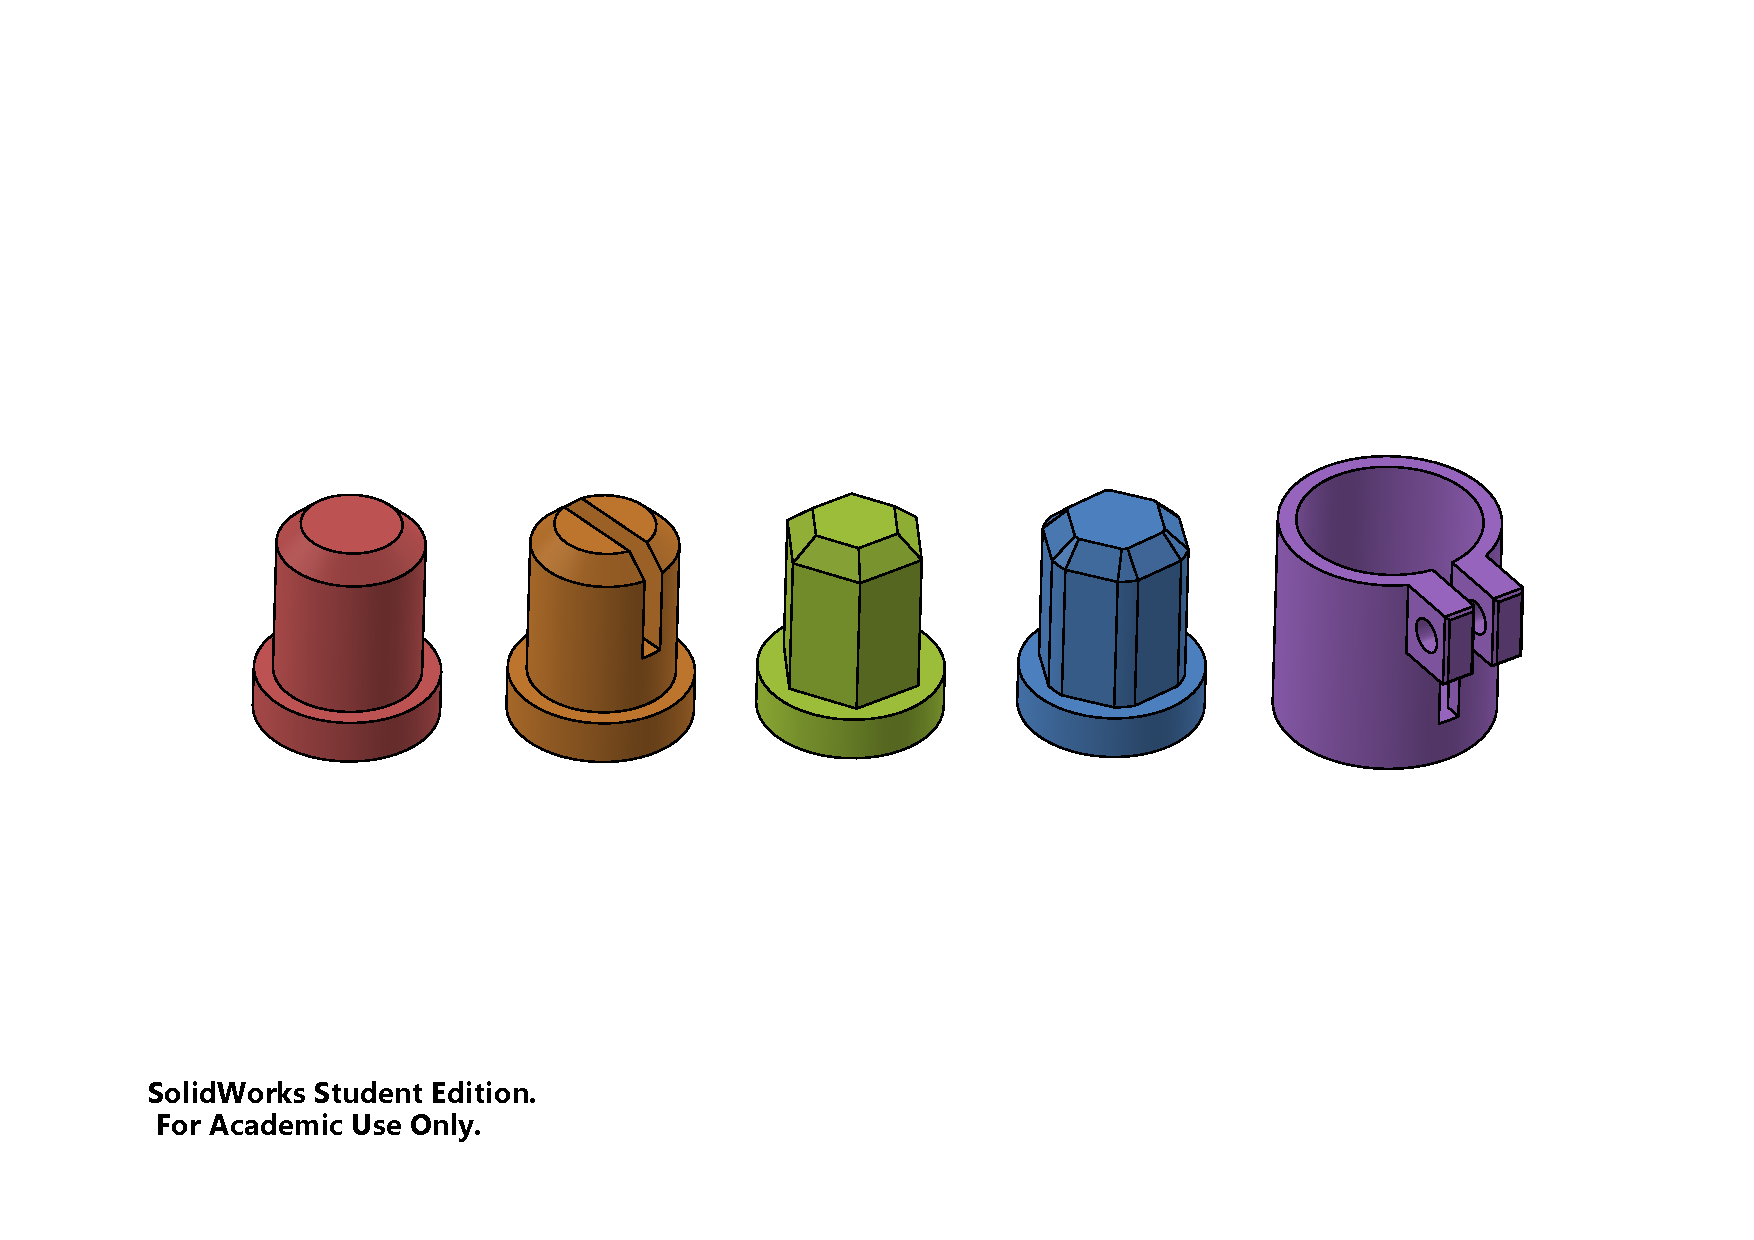
\includegraphics[clip, trim=3cm 6cm 3cm 6cm, width=1\linewidth]{figures/plug-concepts}
        \caption[Render of the plug concepts considered for the attachment of aluminium shafts onto joints and pivots]{Render of the plug concepts considered for the attachment of aluminium shafts onto joints and pivots}
        \label{fig:mechDesign-plugConcepts}
        \end{figure}
        
        % TODO: Label the plugs
        
        The plug that was selected was hexagonal in shape but had edges which were filleted to match the inside surface of the aluminium tube. This was a hybridisation of the cylindrical plug, which introduced a very low window of tolerance in the manufacture of the joints, and the simple hexagonal plug. The filleted edges increased the contact surface area with the inside of the tube, improving the effectiveness of the fit, whilst allowing for greater manufacturing tolerances. In case the plugs proved to be lacking the required strength, a hole could have been drilled down the centre of the plug and a steel rod could be glued into place to strengthen the joint, specifically at the intersection of the middle body and the plug. A nut and bolt were added to the plug-tube assembly as in Figure~\ref{fig:mechDesign-plugTubeBearingDetail} to improve the fitting and prevent rotation of the tube around the axis of the plug.
        
        \begin{figure}[h!]
          \centering
          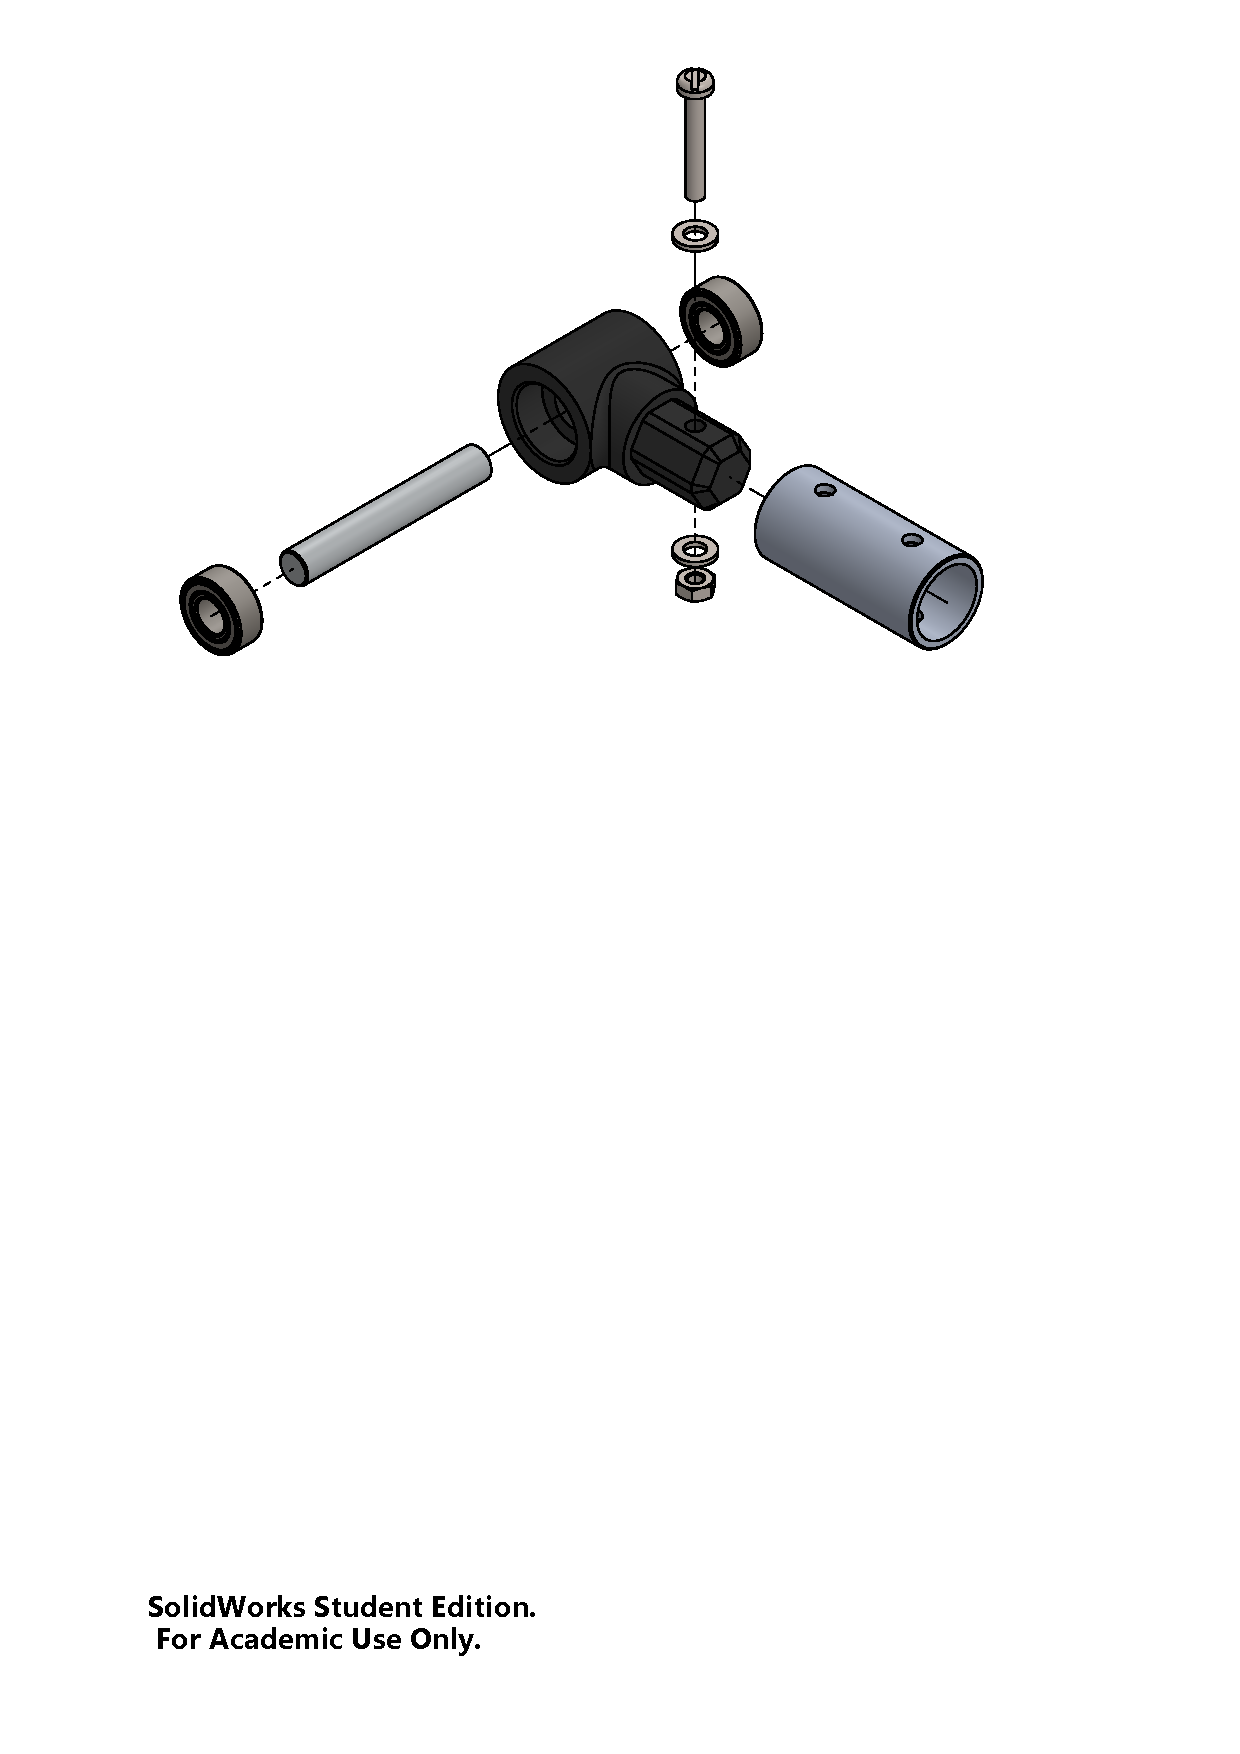
\includegraphics[clip, trim=2cm 17cm 2cm 1cm, width=0.8\linewidth]{figures/plug-tube-bearing}
          \caption[An isometric exploded view of the plug-tube-bearing assembly concept for the suspension system]{An isometric exploded view of the plug-tube-bearing assembly concept for the suspension system}
          \label{fig:mechDesign-plugTubeBearingDetail}
        \end{figure}        
        
        An extension to the rocker joint was made in the form of a ``fin'' feature to allow for the connection of the differential system. The feature was added ``in-place'' in the 3D model after the differential had been added to the assembly so that correct alignment was ensured.
        
        Finally, features for the press-fitting of bearings were added to the joints that required them. Bearings were chosen at this point to be of dimensions shown in Figure~\ref{fig:mechDesign-bearingShaftDetail} in which the shaft diameter is also shown. A single bearing alone was not suitable to provide support against bending torques brought about when the shafts were to be put under load, thus each free-moving joint had two bearings on either extremity. A hole through the centre of the bearing bores of $\diameter8$ mm was included to allow the shafts to extend to the outward-facing bearings. The final designs for each of the three joints are shown in Figures~\ref{fig:mechDesign-rockerJointDetail}, \ref{fig:mechDesign-bogieJointFixedDetail} and \ref{fig:mechDesign-bogieJointFreeDetail}.
        
        \begin{figure}[h!]
          \centering
          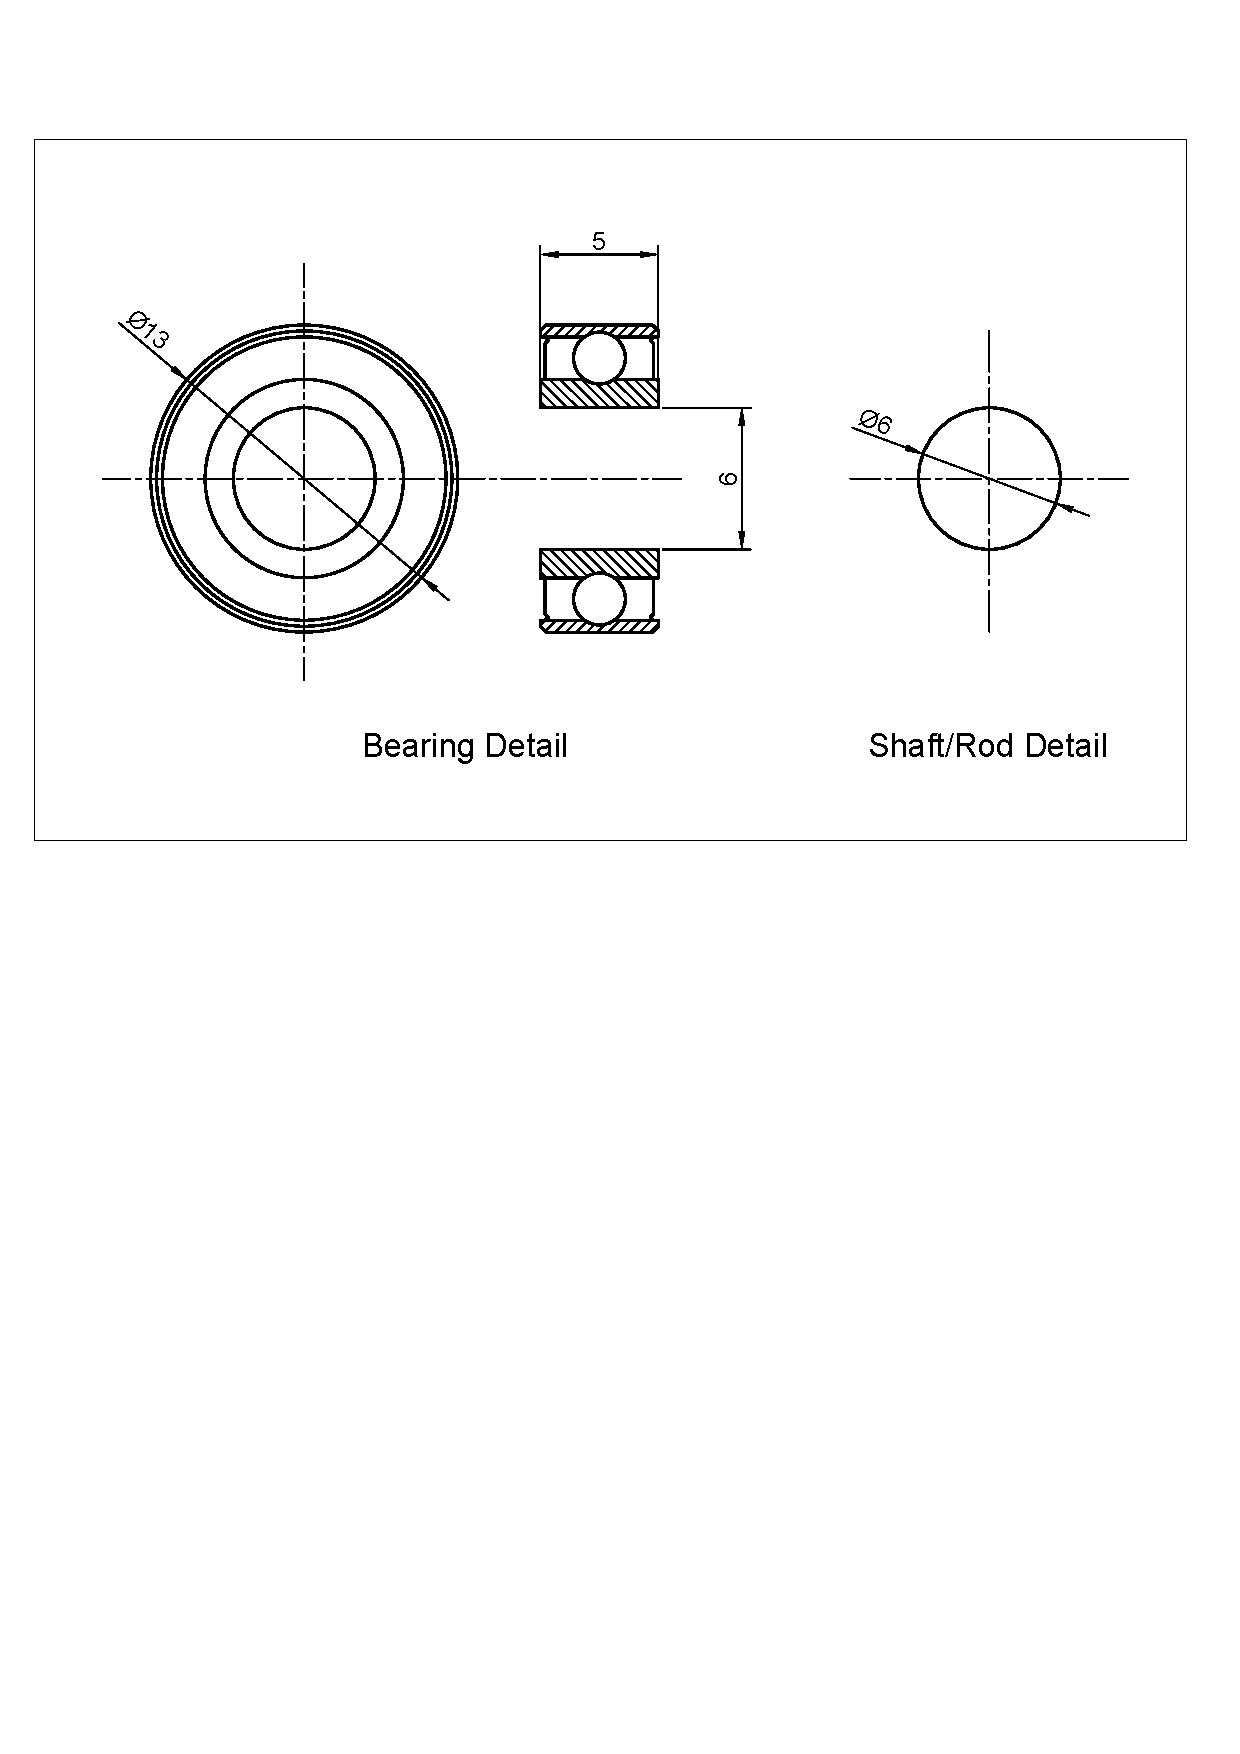
\includegraphics[clip, trim=2cm 16cm 2cm 3cm, width=0.7\linewidth]{figures/bearing-shaft-detail}
          \caption[Detail of the bearings and shaft chosen for all applicable areas]{Detail of the bearings and shaft chosen for all applicable areas}
          \label{fig:mechDesign-bearingShaftDetail}
        \end{figure}        
        
        \begin{figure}[h!]
        \centering
        \subfloat[]{
          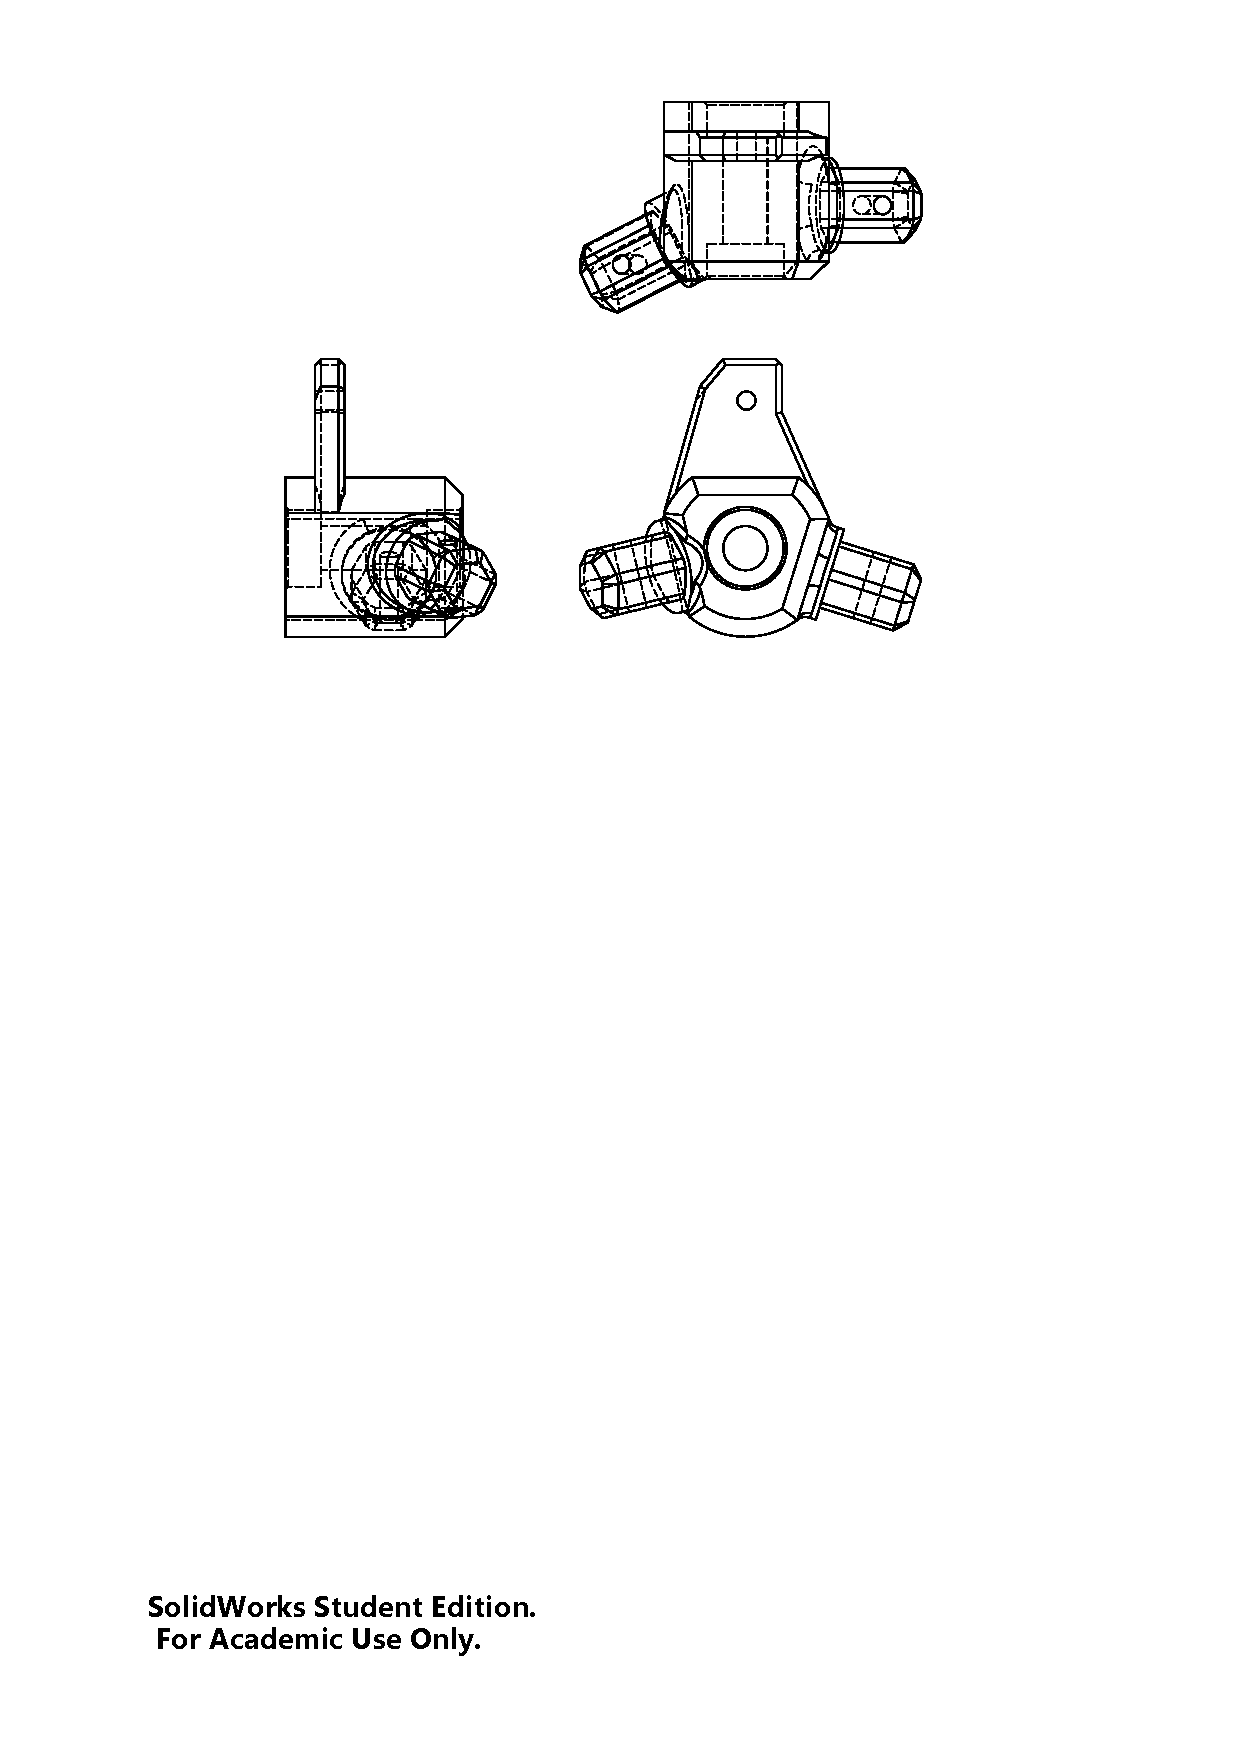
\includegraphics[clip, trim=4cm 18cm 4cm 1cm, width=.59\linewidth]{figures/rocker-joint.PDF}
        }
        \subfloat[]{
          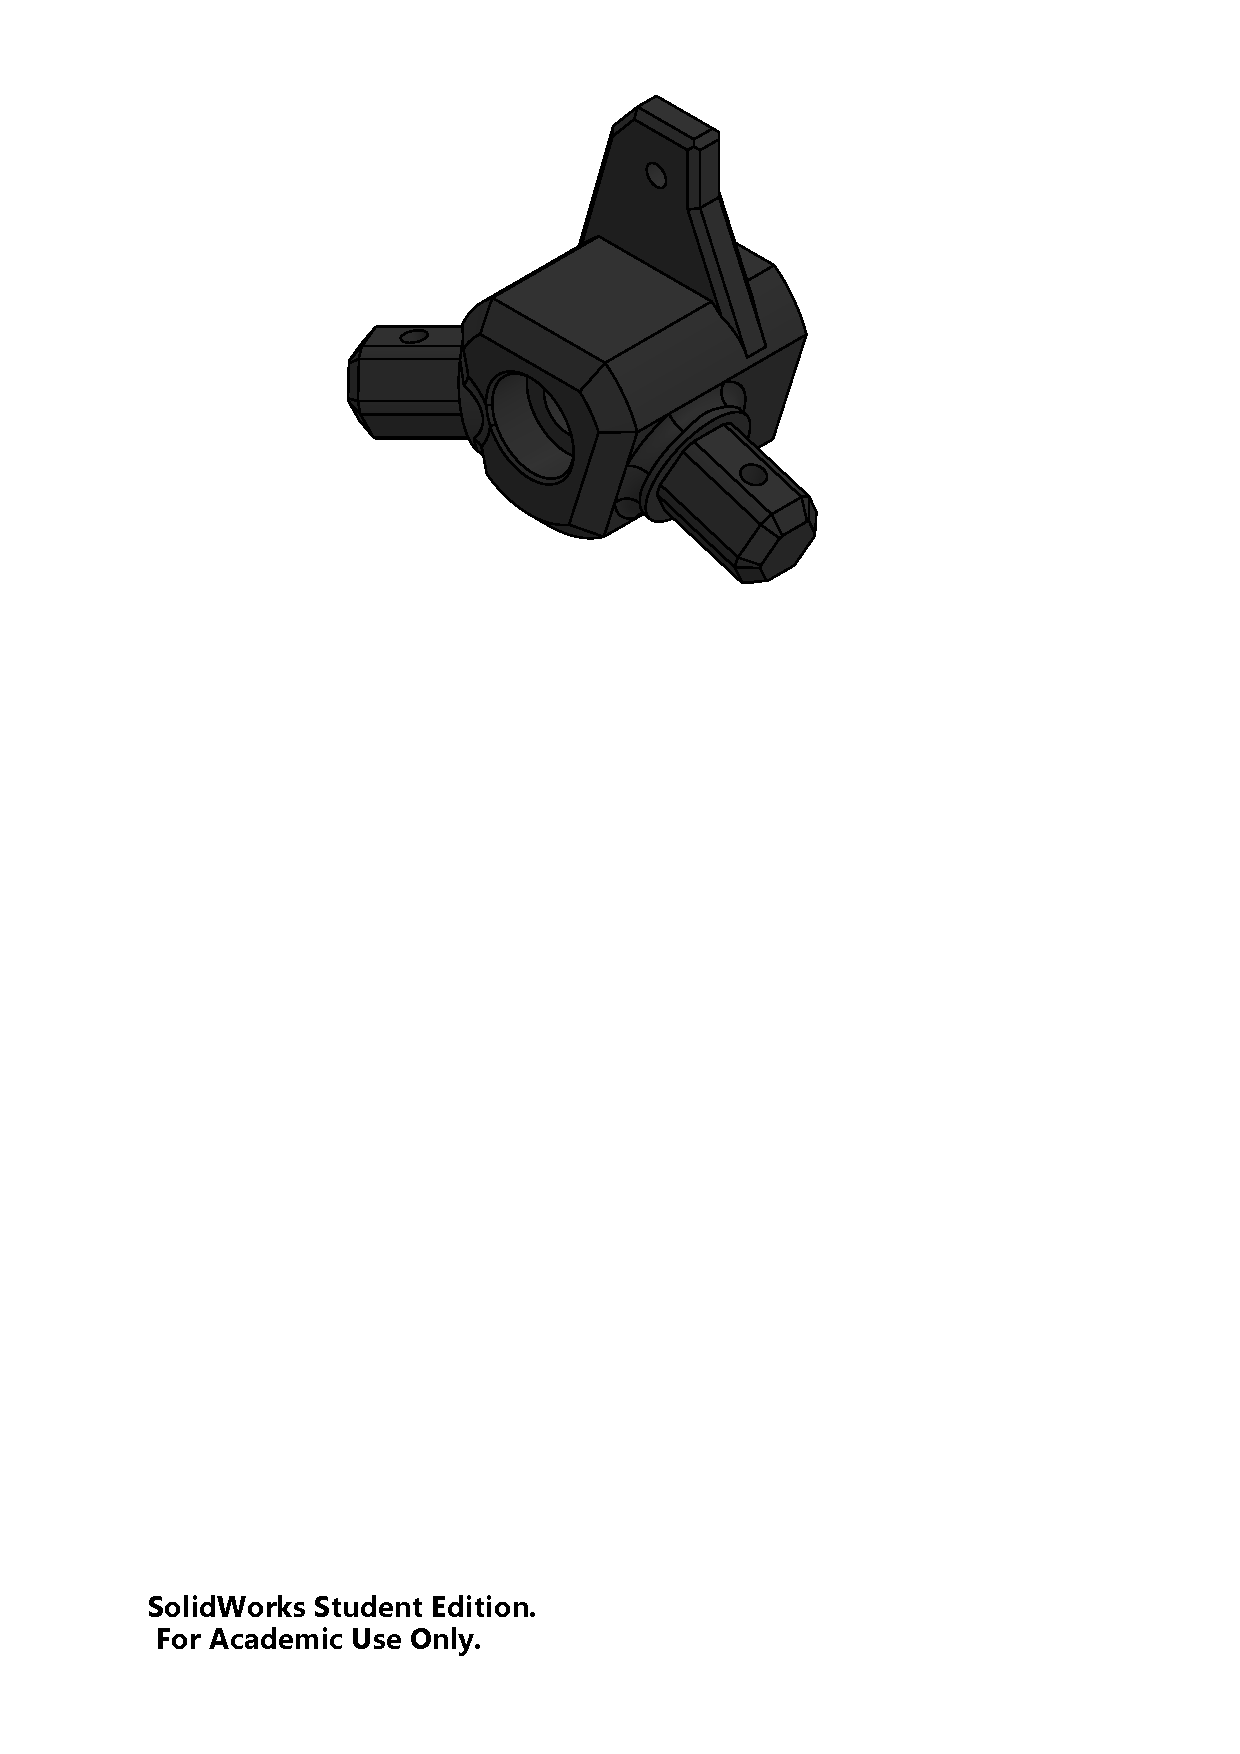
\includegraphics[clip, trim=6cm 18cm 6cm 1cm, width=.4\linewidth]{figures/rocker-joint-iso.PDF}
        }
        \caption[Detailed drawings of the rocker joint component for one side of the suspension system]{Detailed drawings of the rocker joint component for one side of the suspension system}
        \label{fig:mechDesign-rockerJointDetail}
        \end{figure}
        
        \begin{figure}[h!]
        \centering
        \subfloat[]{
          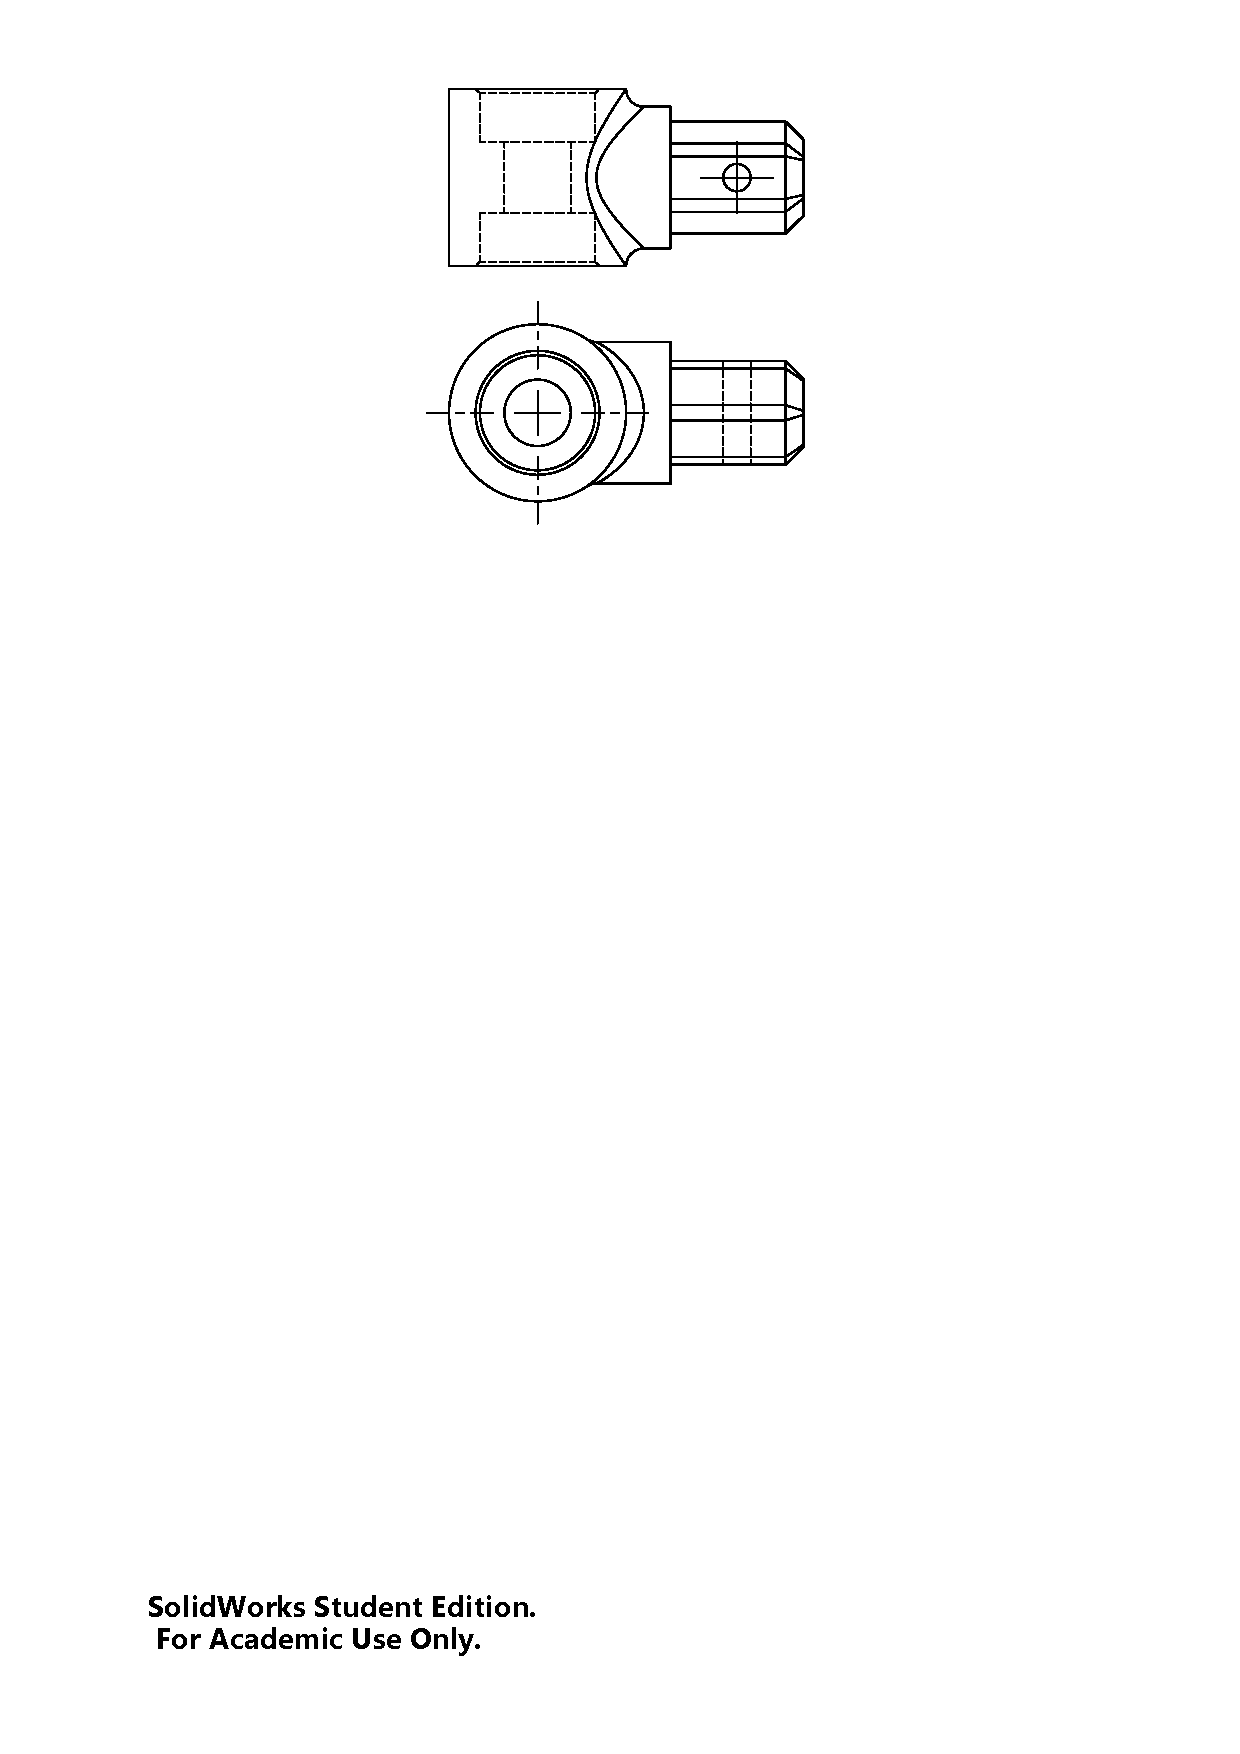
\includegraphics[clip, trim=6cm 18cm 6cm 1cm, width=.45\linewidth]{figures/bogie-joint-free.PDF}
        }
        \subfloat[]{
          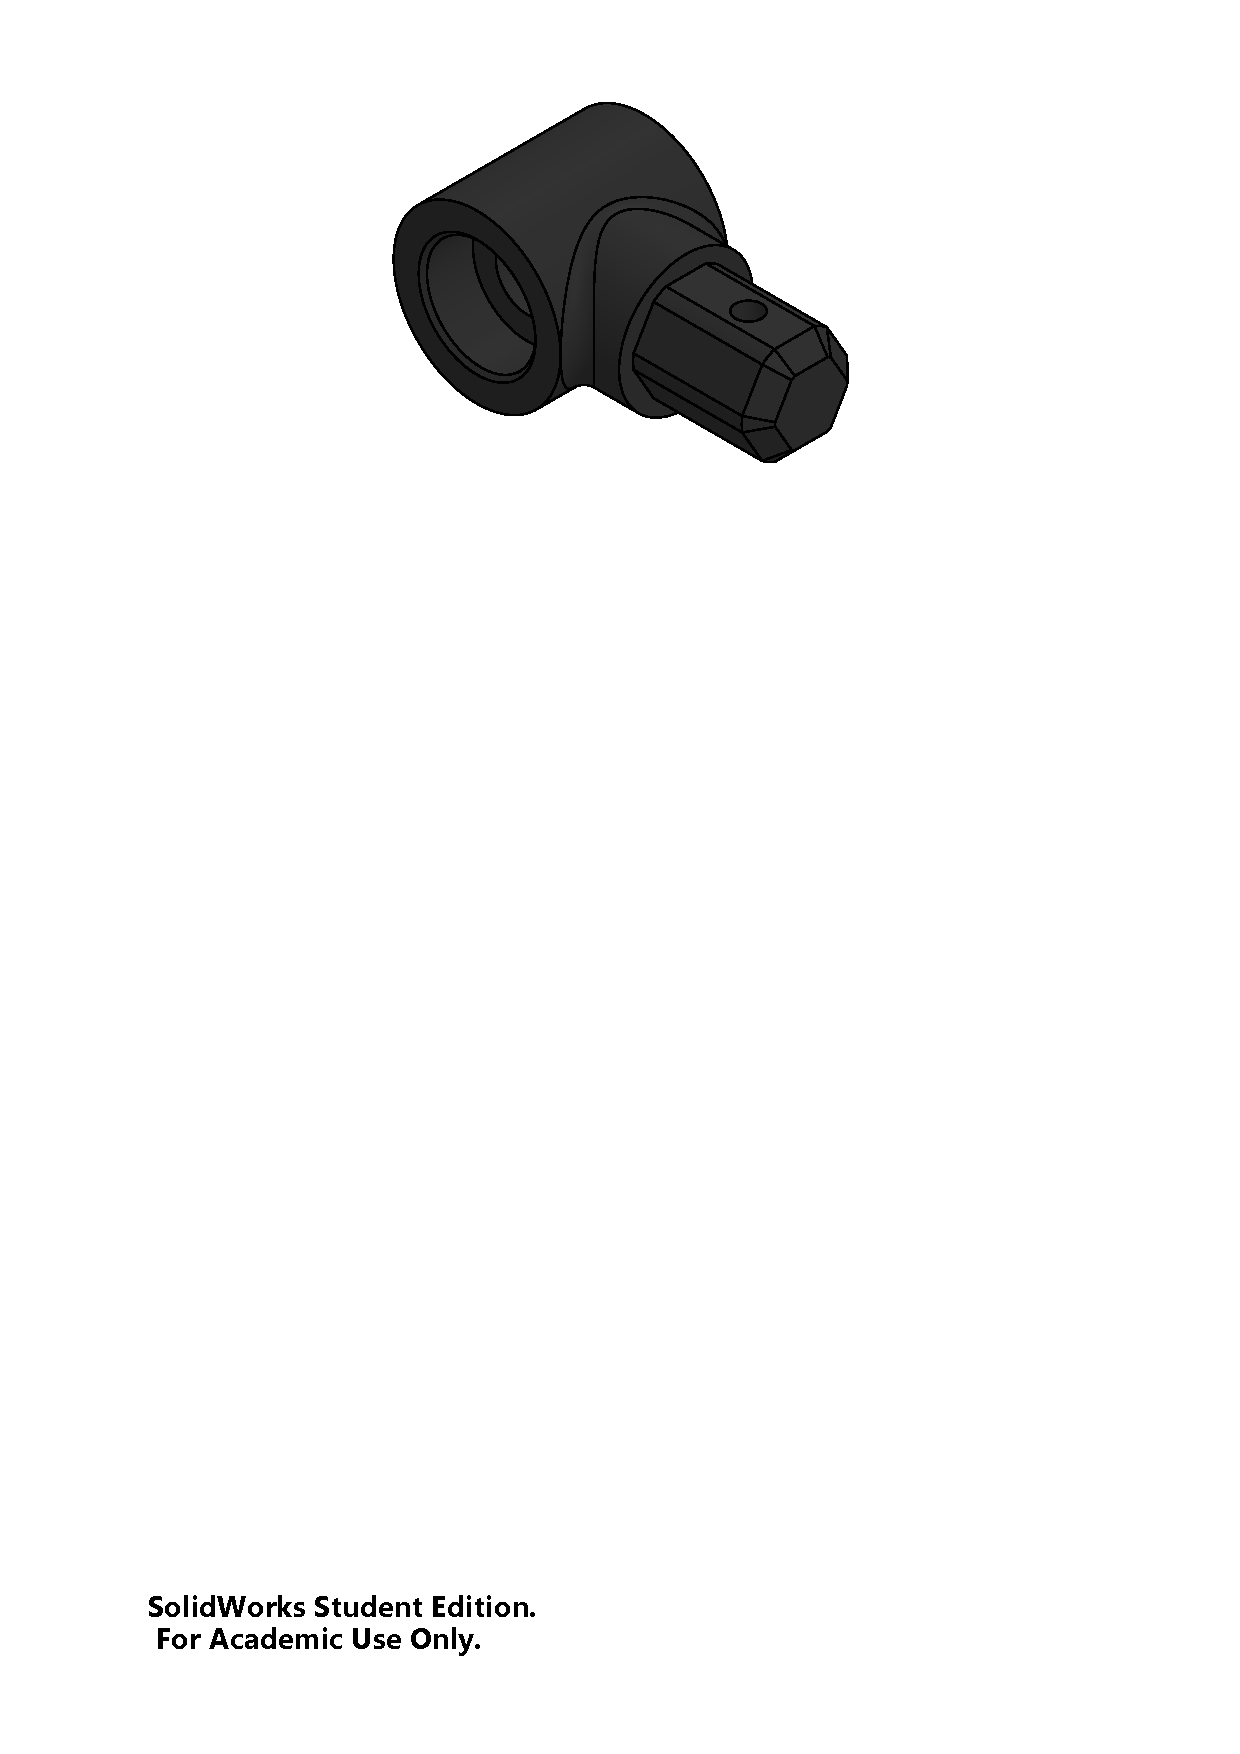
\includegraphics[clip, trim=6cm 18cm 6cm 1cm, width=.45\linewidth]{figures/bogie-joint-free-iso.PDF}
        }
        \caption[Detailed drawings of the free bogie joint component for one side of the suspension system]{Detailed drawings of the free bogie joint component for one side of the suspension system}
        \label{fig:mechDesign-bogieJointFreeDetail}
        \end{figure}
        
        \begin{figure}[h!]
        \centering
        \subfloat[]{
          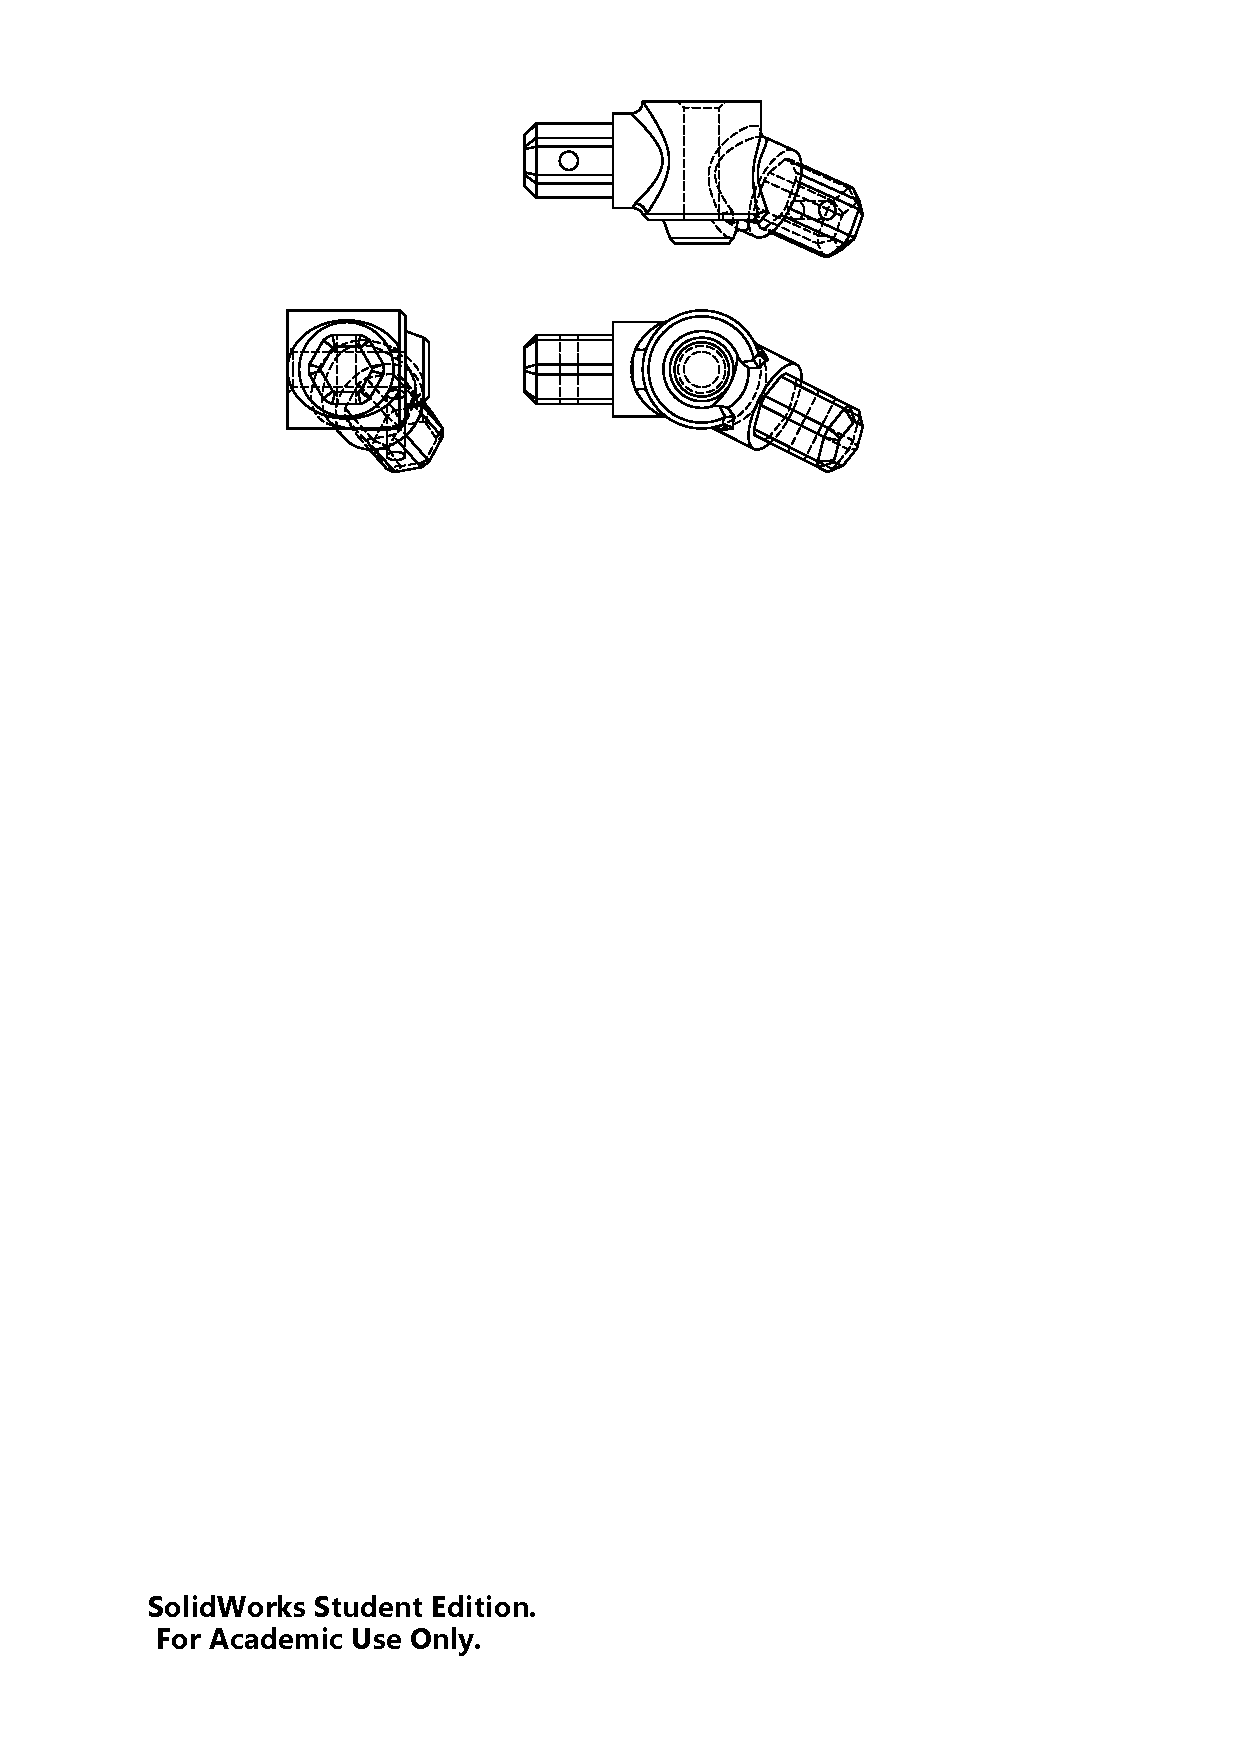
\includegraphics[clip, trim=4cm 20cm 4cm 1cm, width=.65\linewidth]{figures/bogie-joint-fixed.PDF}
        }
        \subfloat[]{
          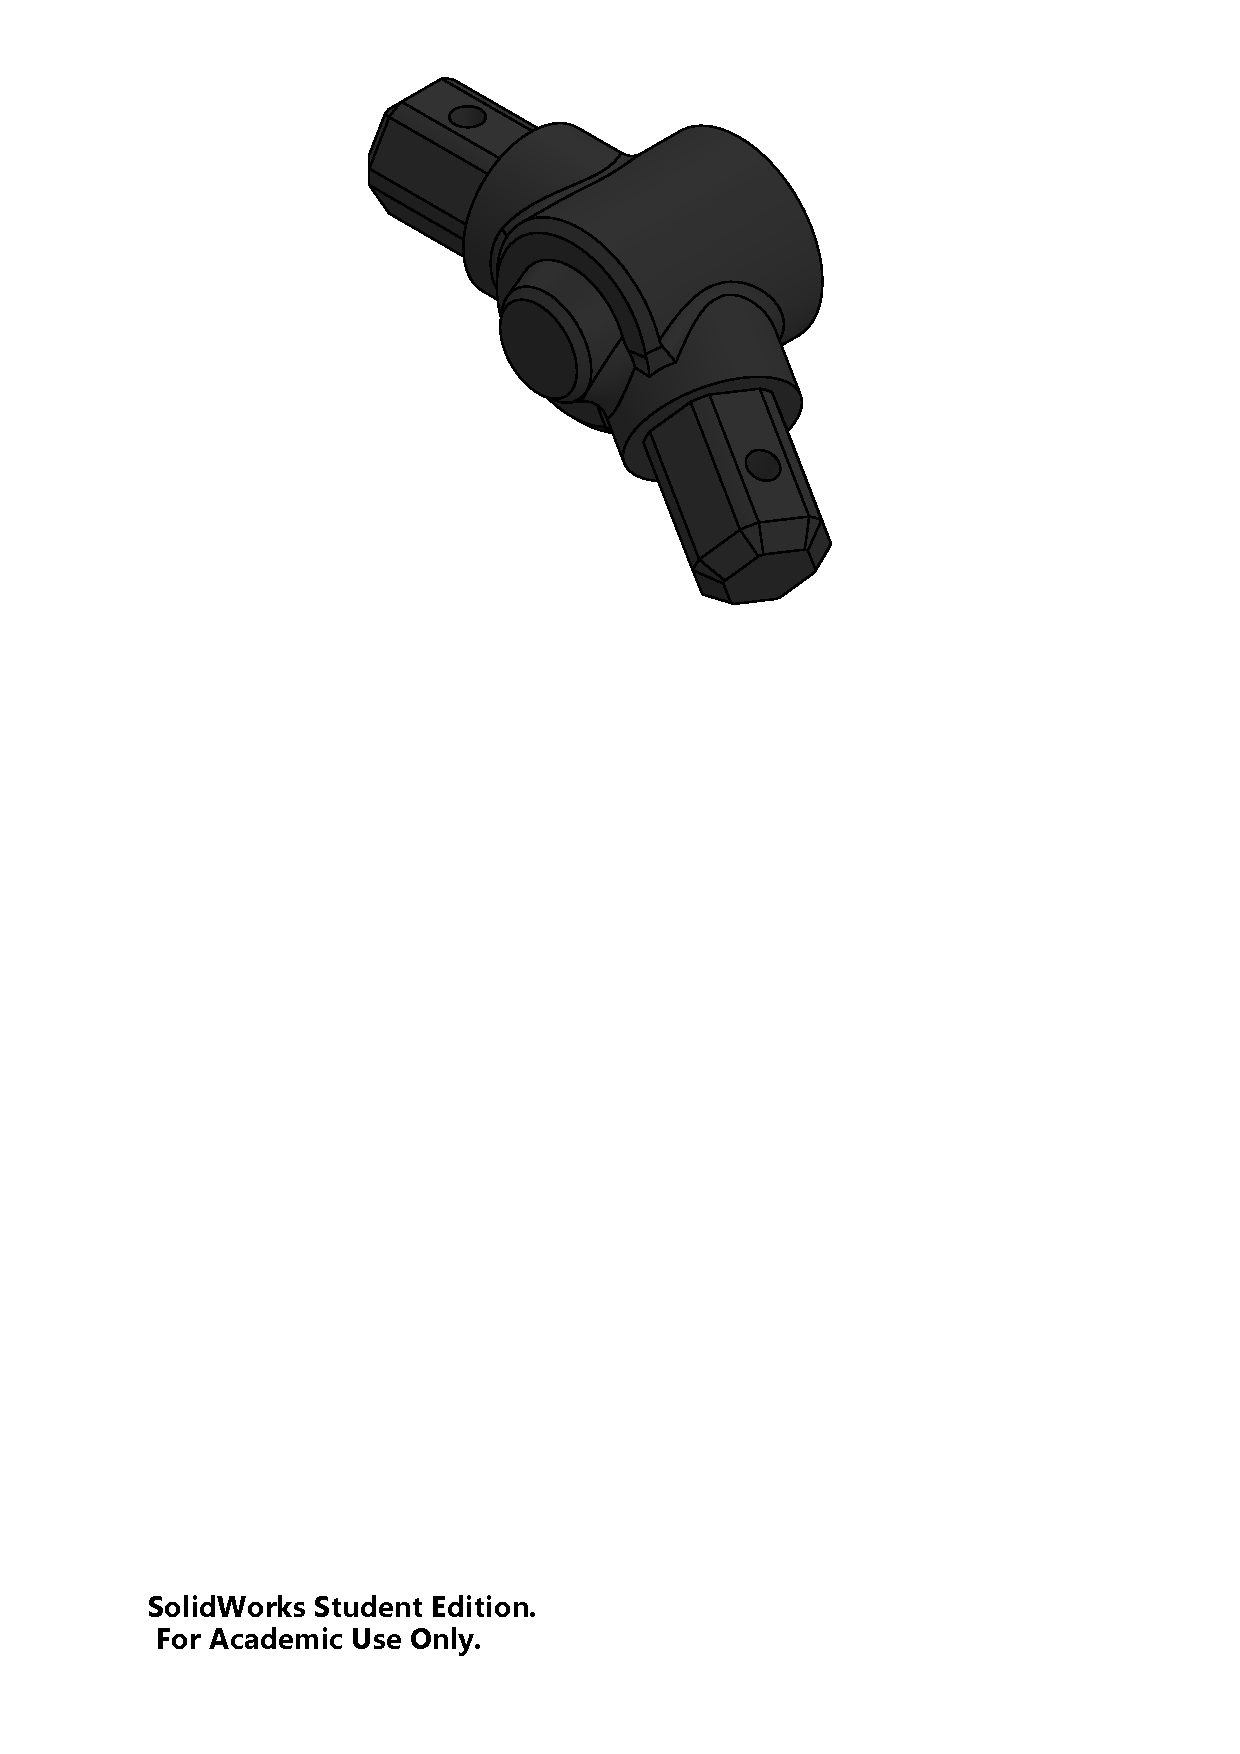
\includegraphics[clip, trim=6cm 18cm 6cm 1cm, width=.34\linewidth]{figures/bogie-joint-fixed-iso.PDF}
        }
        \caption[Detailed drawings of the fixed bogie joint component for one side of the suspension system]{Detailed drawings of the fixed bogie joint component for one side of the suspension system}
        \label{fig:mechDesign-bogieJointFixedDetail}
        \end{figure}
        
      \subheading{Wheels}\\\\
        Six wheels were to be designed, four of which were driven by the sub-micro servos (front and rear wheels) and the two centre wheels were to be mounted onto fixed shafts with bearings. All six of the wheels on the real \textit{Curiosity} are actuated to ensure robustness of the driving mechanisms in a wider range of terrain types and traversal situations. It is also a feature of redundancy in that if one of the motors fails, the rover is capable of continuing operation. However, it was decided that for this model only the front and rear wheels would be actuated given the reduced power to weight ratio compared to that of \textit{Curiosity}. Redundancy was not an issue worth the resultant extra servos and the incurred additional control complexity.
        
        As mentioned in Section~\ref{subsec:rover-concept-proposals}, the wheels were a great opportunity to make use of the aesthetic accuracy of additive manufacturing thus the wheel was modelled so as to replicate the cross-sectional curve of the outer shell of the wheel. Included were the tread patterns for traction as well as the morse-code emboss which read ``JPL'', used on \textit{Curiosity} to acquire optical estimates of the distance travelled by the rover. Spokes and a centre cylindrical core was added to the inside of the outer shell, keeping the wheel as a single piece.
        
        The sub-micro servos were accompanied by servo horns that fitted onto the shaft of the servo. The horns were cross-shaped, a layout of which was taken advantage to provide support in the cross-axis plane. The horns were measured and holes were added to the four wheels concerned so that they could be mounted directly to the driving servos. The need for bearings on this assembly was countered by an estimate of the forces developed due to the rover's weight and it was determined that the servos would be capable of taking the estimated load without damage or wear. This also provisioned for easy replacement of wheels and or servos should one of them be damaged.
        
        The same bearing bores and centre hole as on the joint components was added to the cylindrical core of the centre wheels for mounting to the aluminium shafts. The press-fitting of bearings into the wheels was to be of the same nature as that of the joints. Figures~\ref{fig:mechDesign-outerWheelDetail} and \ref{fig:mechDesign-midWheelDetail} show the outer and centre wheel details.
        
        \begin{figure}[h!]
        \centering
        \subfloat[]{
          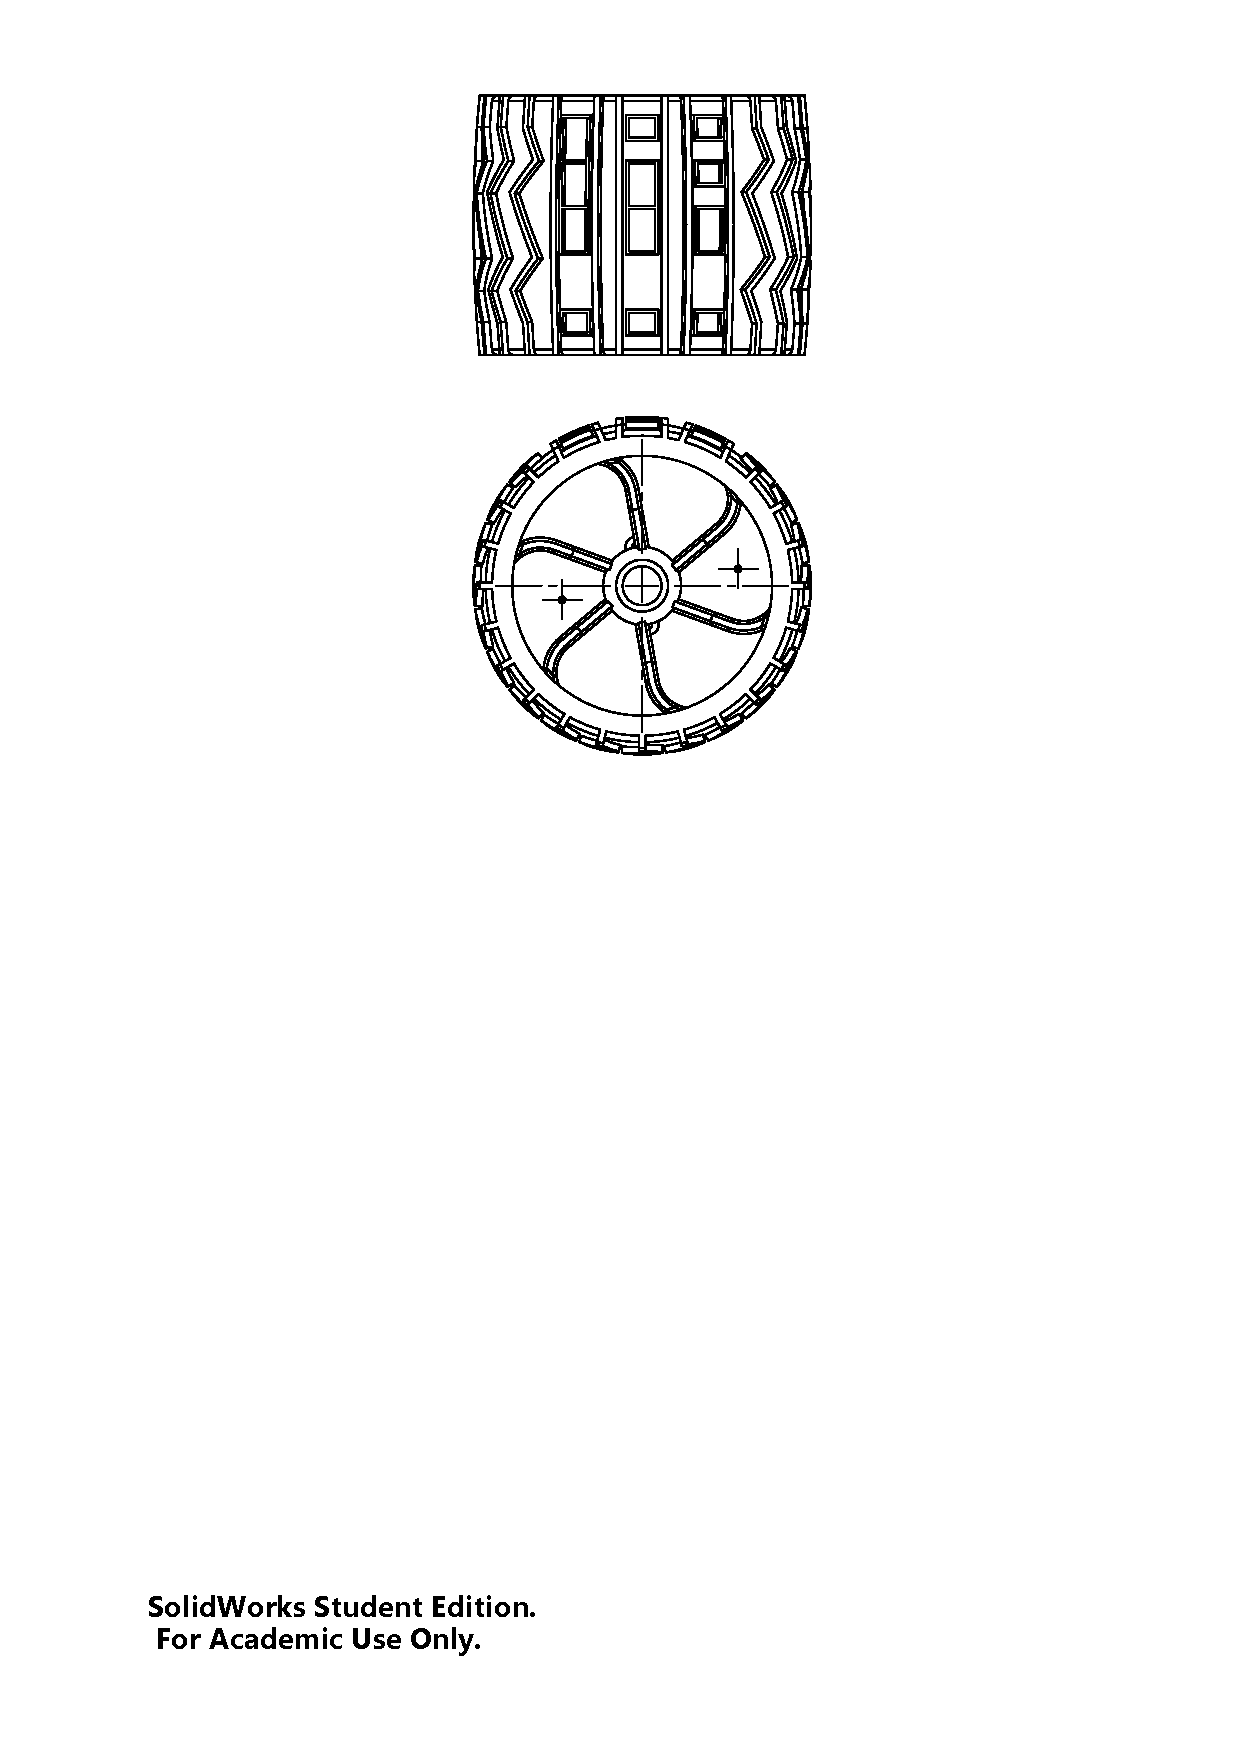
\includegraphics[clip, trim=6cm 16cm 6cm 1cm, width=.5\linewidth]{figures/tire-outer}
        }
        \qquad
        \subfloat[]{
          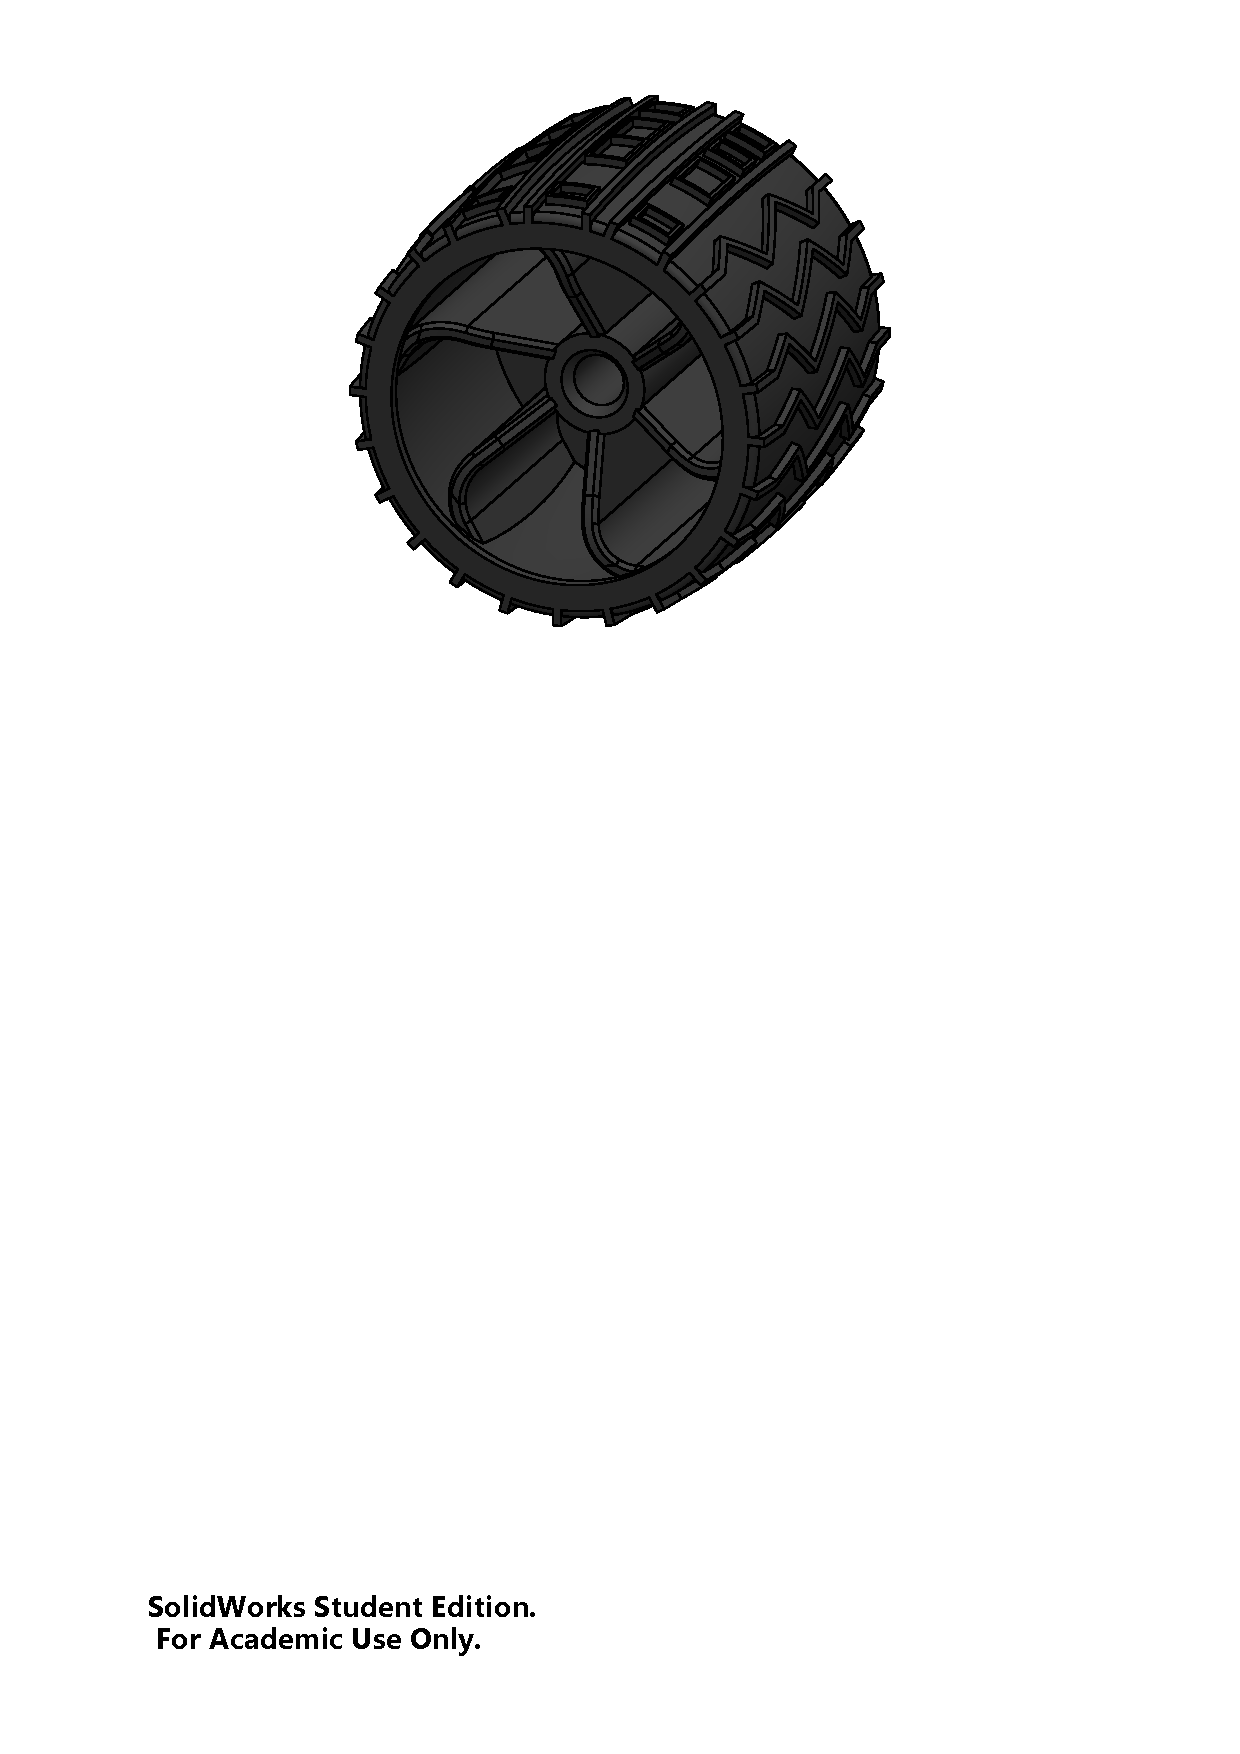
\includegraphics[clip, trim=6cm 16cm 6cm 1cm, width=.4\linewidth]{figures/tire-outer-dimet}
        }
        \caption[Detailed drawings of the leading and trailing wheels]{Detailed drawings of the leading and trailing wheels}
        \label{fig:mechDesign-outerWheelDetail}
        \end{figure}
        
        \begin{figure}[h!]
        \centering
        \subfloat[]{
          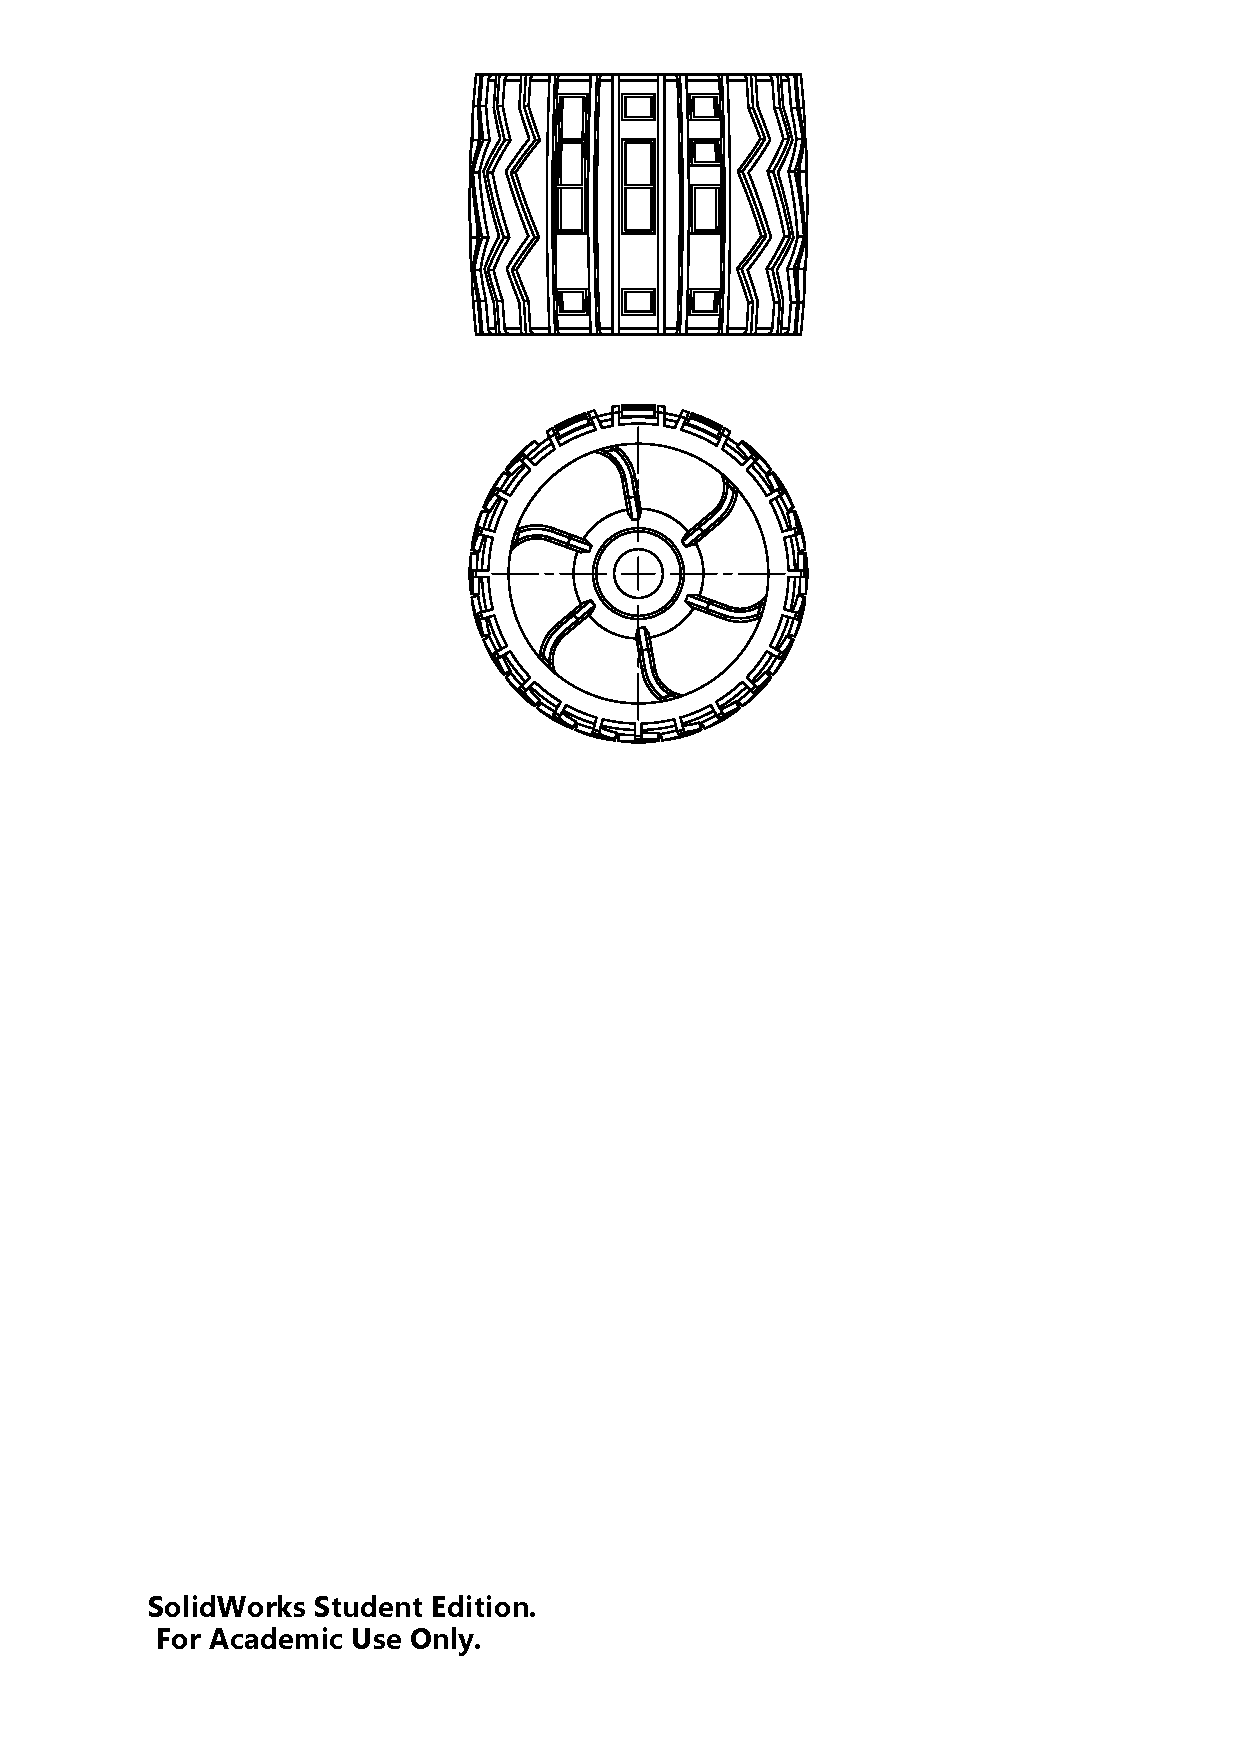
\includegraphics[clip, trim=6cm 16cm 6cm 1cm, width=.5\linewidth]{figures/tire-mid}
        }
        \qquad
        \subfloat[]{
          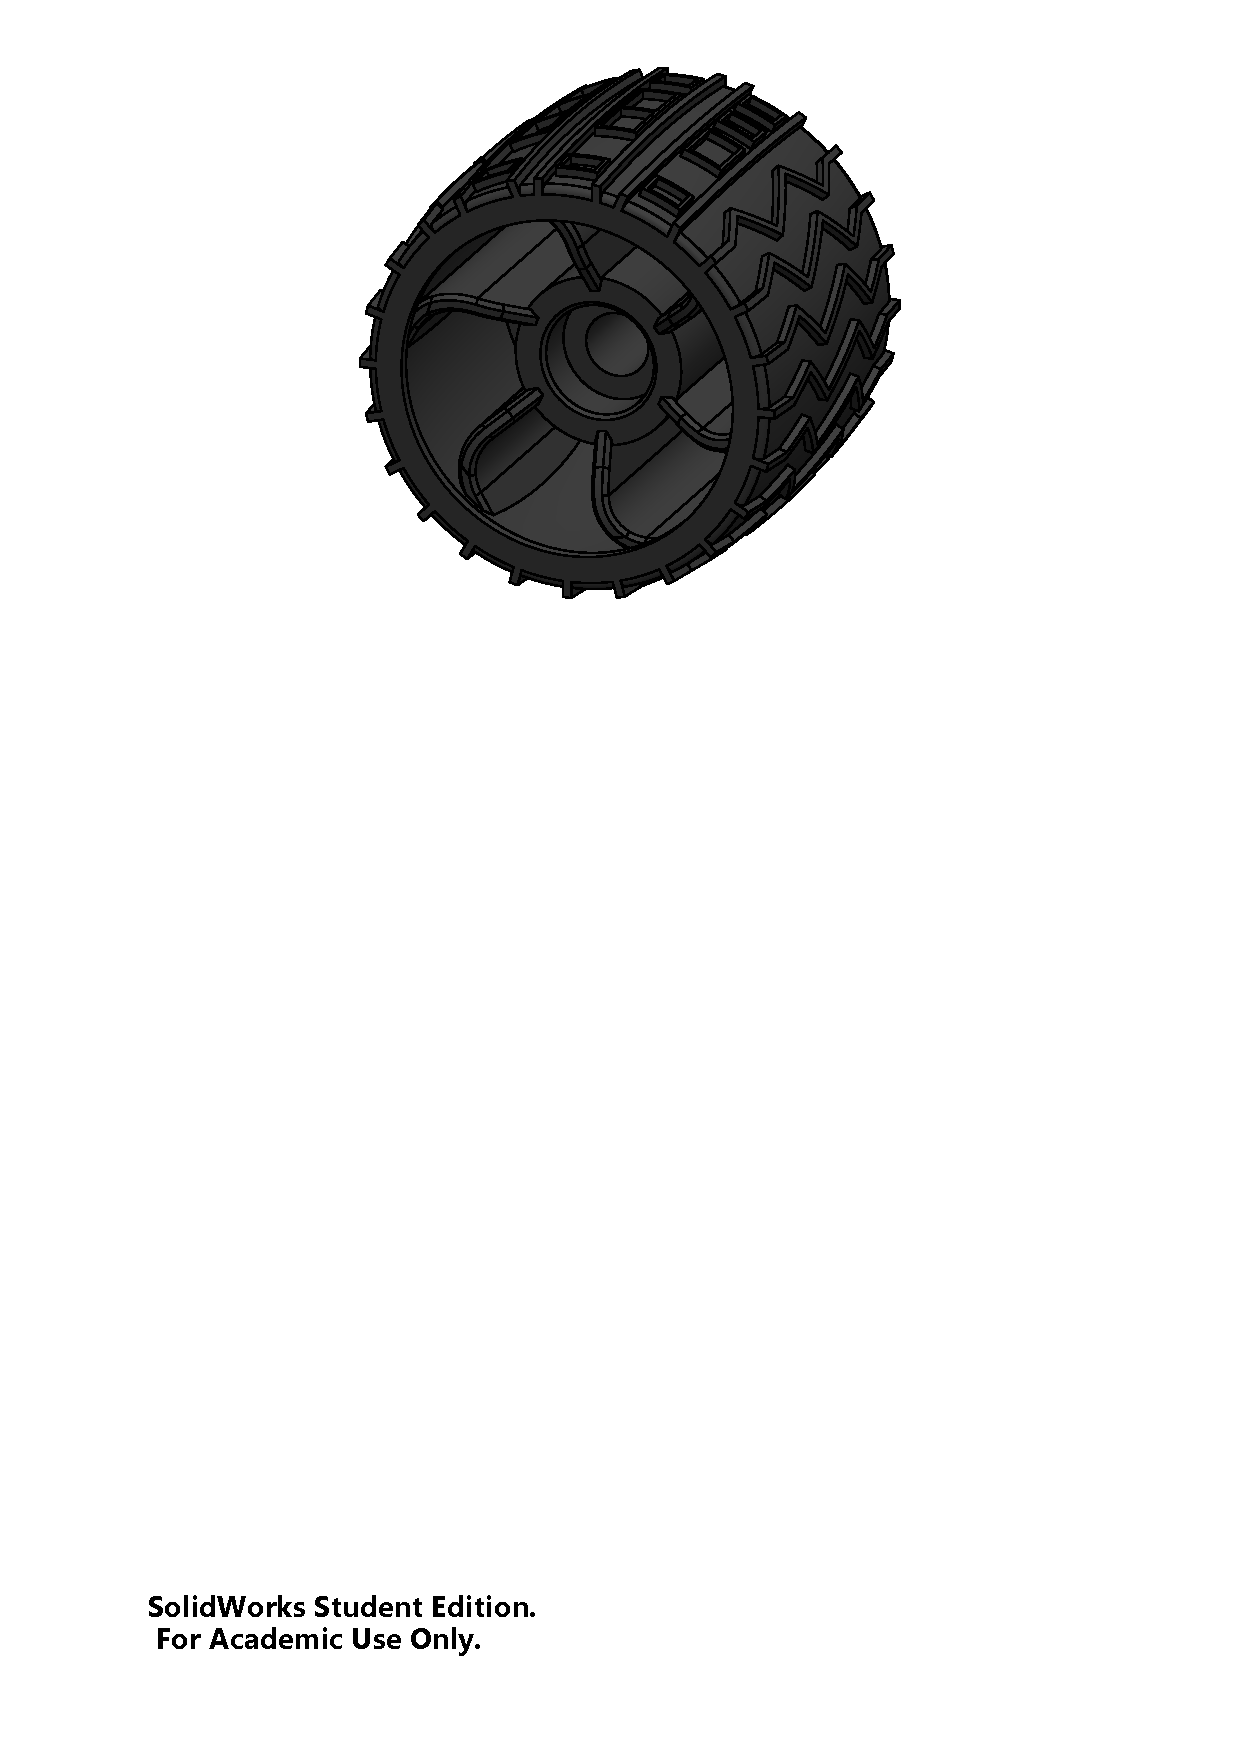
\includegraphics[clip, trim=6cm 16cm 5cm 1cm, width=.4\linewidth]{figures/tire-mid-dimet}
        }
        \caption[Detailed drawings of the centre wheels]{Detailed drawings of the centre wheels}
        \label{fig:mechDesign-midWheelDetail}
        \end{figure}
          
      \subheading{Pivots}\\\\
        Turning the wheel-strut assembly involved the pivot component which had to allow for mounting of a sub-micro steering servo and for attachment to the ends of the fore rocker-tubes and aft bogie-tubes. The same concept for attaching to the aluminium tube as in the case of the joints was applied to the pivots. Thus the design consisted of a L-shaped extrusion with the plug extending from one of the outside flat surfaces. The other surface had a rectangular cut-out the size of the servo body, mounting holes for the servo and ribs for supporting the L-shaped extrusion. Figure~\ref{fig:mechDesign-wheelPivotDetail} shows the pivot component detail for the front wheel assembly.
        
        The front and rear pivots differed slightly due to the different angle of entry of the rocker and bogie tubes towards the centre-points of the wheel assembly. Managing the differences in these angles was aided by use of the 3D skeleton sketch. Again, the front and rear pivots from the left-hand side were mirrored to produce parts for the right-hand side suspension assembly.
       
        \begin{figure}[h!]
        \centering
        \subfloat[]{
          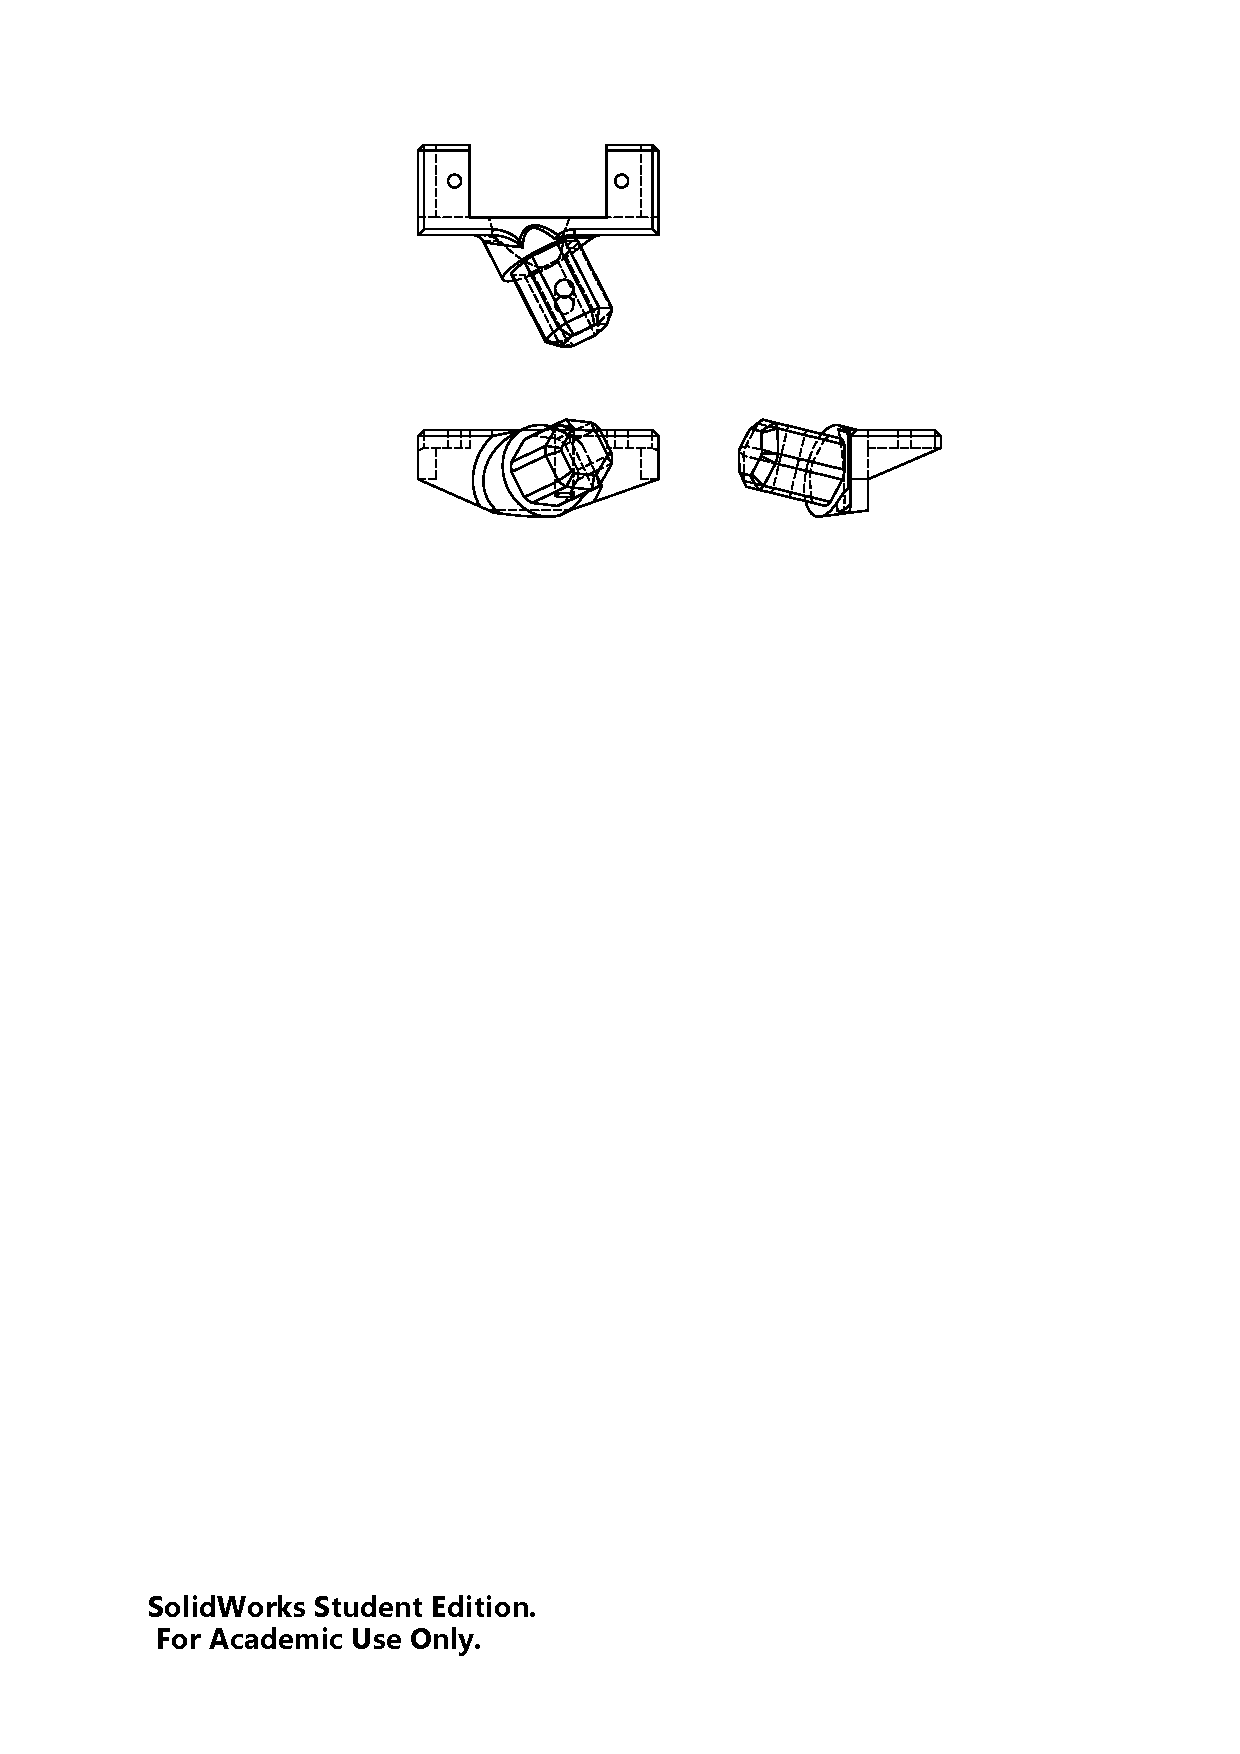
\includegraphics[clip, trim=6cm 20cm 4cm 2cm, width=0.55\linewidth]{figures/wheel-pivot}
        }
        \subfloat[]{
          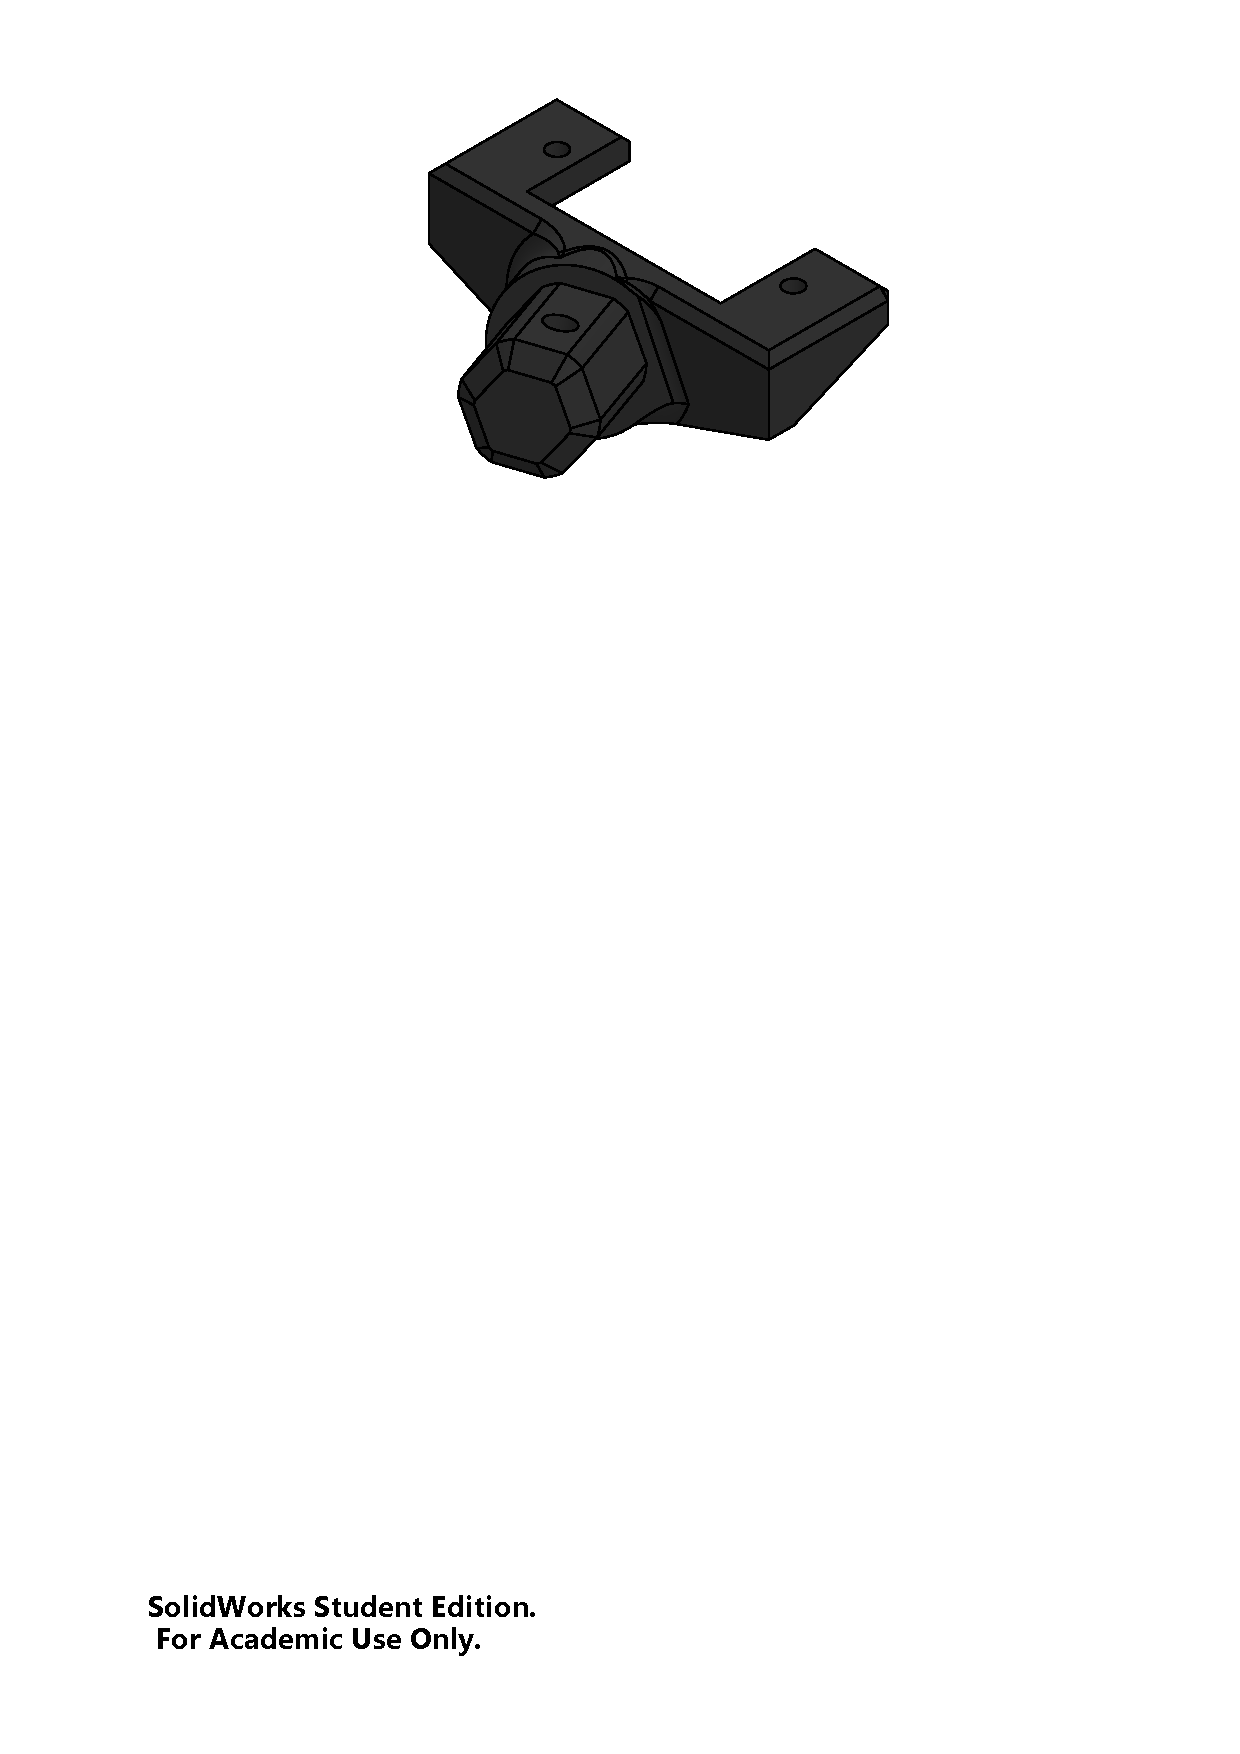
\includegraphics[clip, trim=6cm 20cm 5cm 1cm, width=0.44\linewidth]{figures/wheel-pivot-iso}
        }
        \caption[Detailed drawings of the wheel pivot component for one corner of the suspension system]{Detailed drawings of the wheel pivot component for one corner of the suspension system}
        \label{fig:mechDesign-wheelPivotDetail}
        \end{figure}
          
      \subheading{Struts}\\\\
        \textit{Curiosity} has an arcing ``strut'' for each wheel which curves from above the wheel, underneath the pivot motor, over the side and into the inwards-facing threshold of the hollow of the wheel. The strut is attached to the drive motor on the inside of the wheel, as close as possible to the centre of the wheel for balance and minimisation of bending stress. The sub-micro sized servos would not fit inside the wheels of the model at its chosen scale, thus they had to be mounted on the outside of the wheel. The strut was required to provide a place to mount the driving servo and to be mounted to the servo horns of the steering servo.
        
        The strut was designed to maintain the curved appearance as on \textit{Curiosity} but to take into account the strength of the component. A flat platform above the wheel included holes for mounting the steering servo's horn and this curved downwards into the strut section of the component. The strut curve consisted of a flat section to offer strength against bending in the typical direction as loaded (the $x$-axis) with a rib type extrusion from the rear-facing side of the strut for increased support and tabs on which to mount the driving servo. The design was then mirrored for the rest of the corners and the final detail can be seen in Figure~\ref{fig:mechDesign-wheelStrutDetail}.
        
        \begin{figure}[h!]
        \centering
        \subfloat[]{
          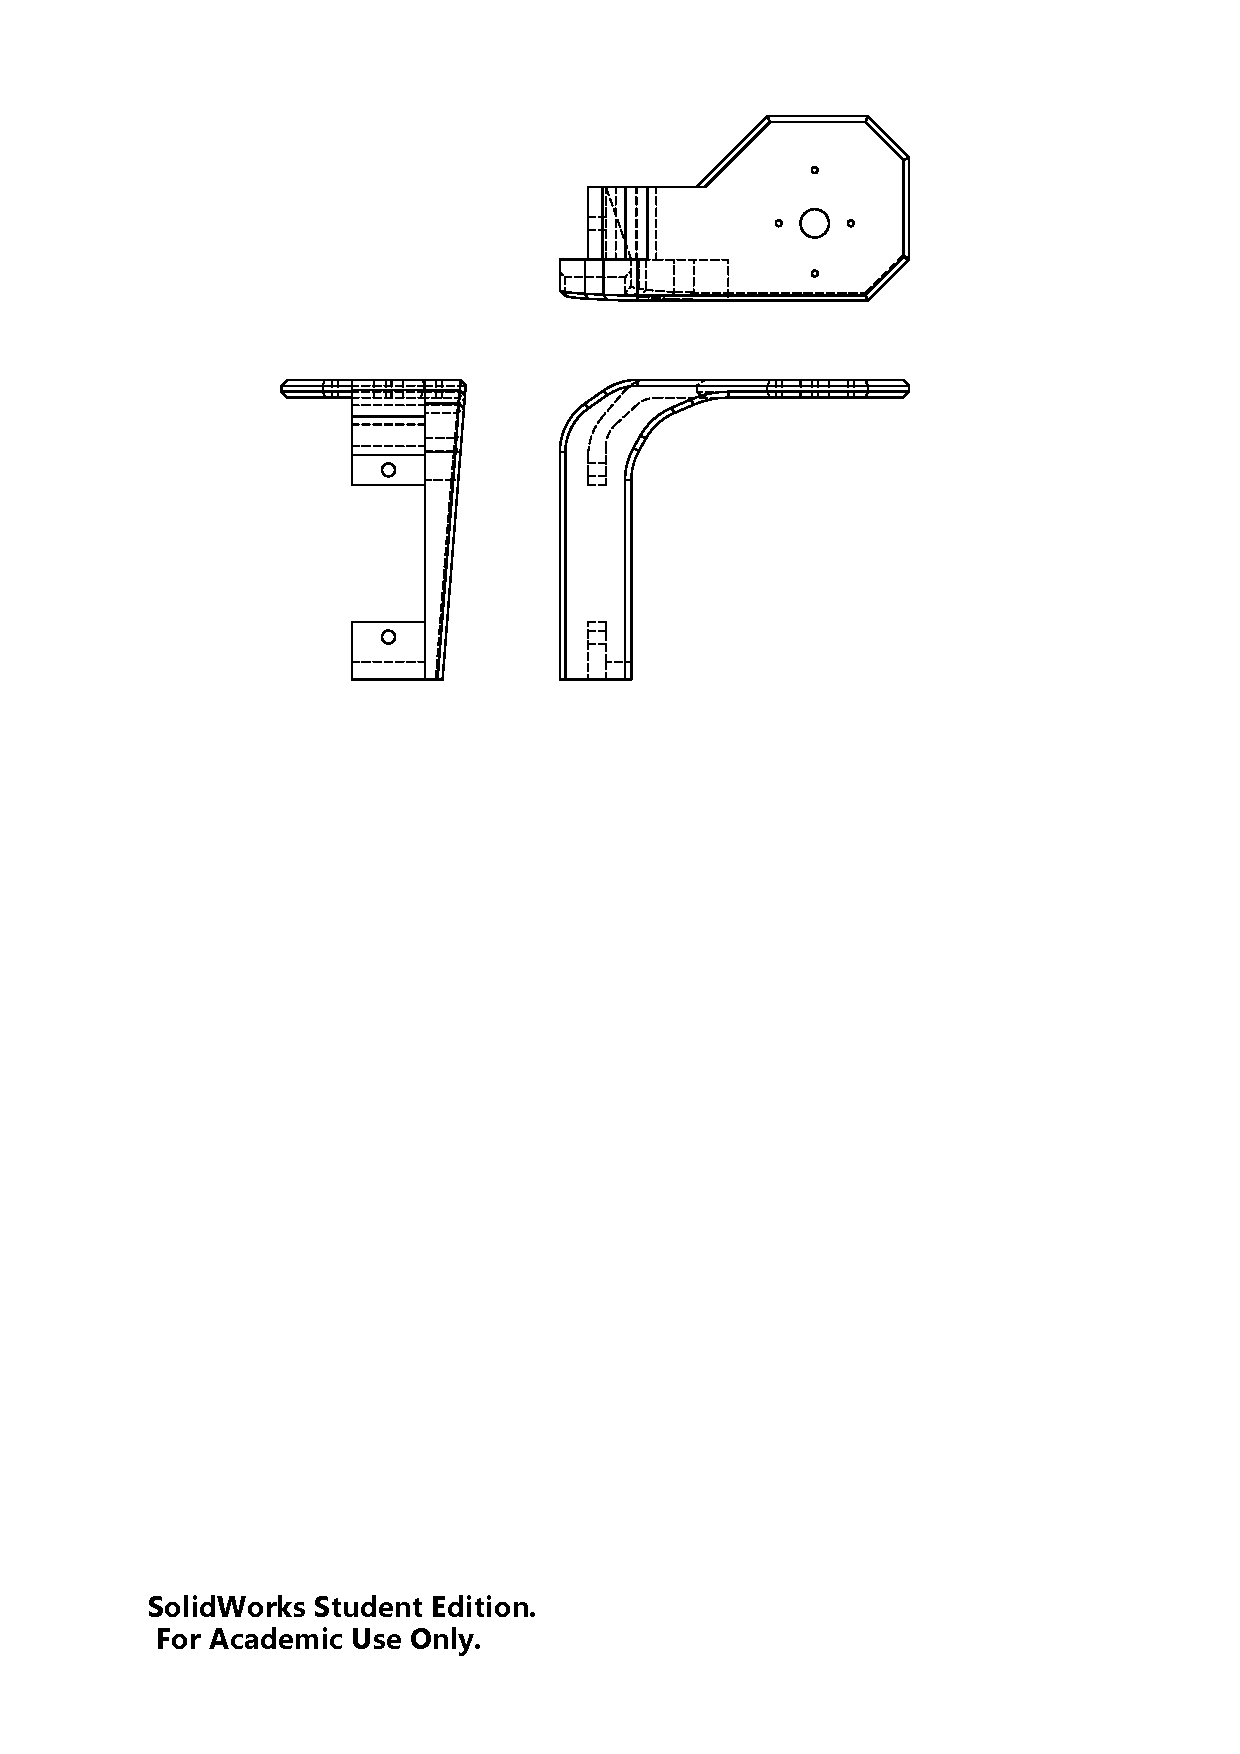
\includegraphics[clip, trim=4cm 17cm 4cm 2cm, width=0.59\linewidth]{figures/wheel-strut}
        }
        \subfloat[]{
          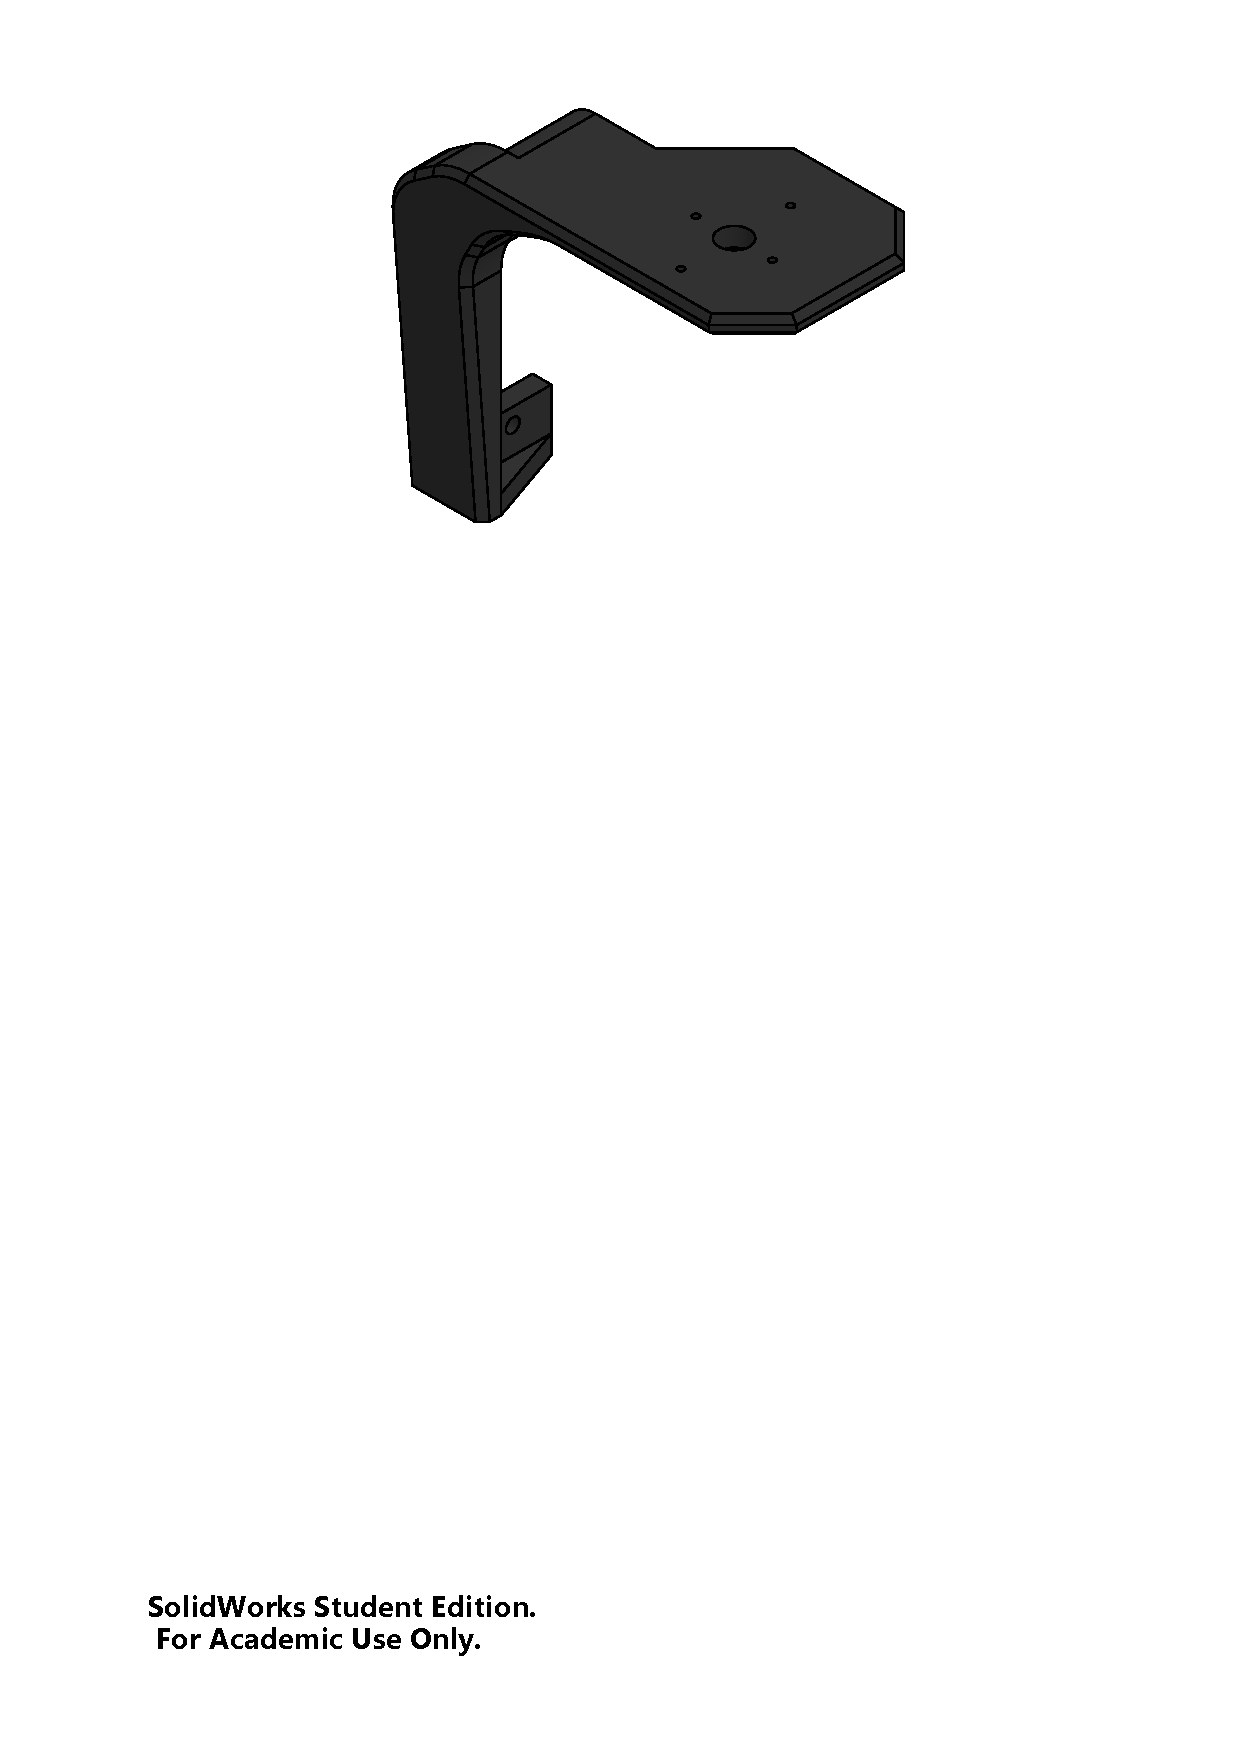
\includegraphics[clip, trim=6cm 19cm 5cm 1cm, width=0.4\linewidth]{figures/wheel-strut-iso}
        }
        \caption[Detailed drawings of the wheel pivot component for one corner of the suspension system]{Detailed drawings of the wheel pivot component for one corner of the suspension system}
        \label{fig:mechDesign-wheelStrutDetail}
        \end{figure}
          
      \subheading{Final Sub-assembly}  

      Having designed the parts around the skeleton sketch, where they were kept fixed to preserve the angle details linking them, another assembly was created, shown in Figure~\ref{fig:mechDesign-suspensionSubDetail} into which the parts were re-added and mated in a manner more typical of the way that they would be assembled. The assembly allowed simulation of the movement and this functionality was used to analyse the assembly for interferences and to ensure that the structure moved the way it was required. Figure~\ref{fig:mechDesign-suspensionSubObstacle} shows the linkages positioned as if the subsystem was navigating over an obstacle. Each individual part was then mirrored and assembled to form the opposite side of the suspension system. The CAD package ensured that the mirrored parts were dynamically updated should one of the original parts have changed.
      
      \begin{figure}[h!]
      \centering
      \subfloat[]{
        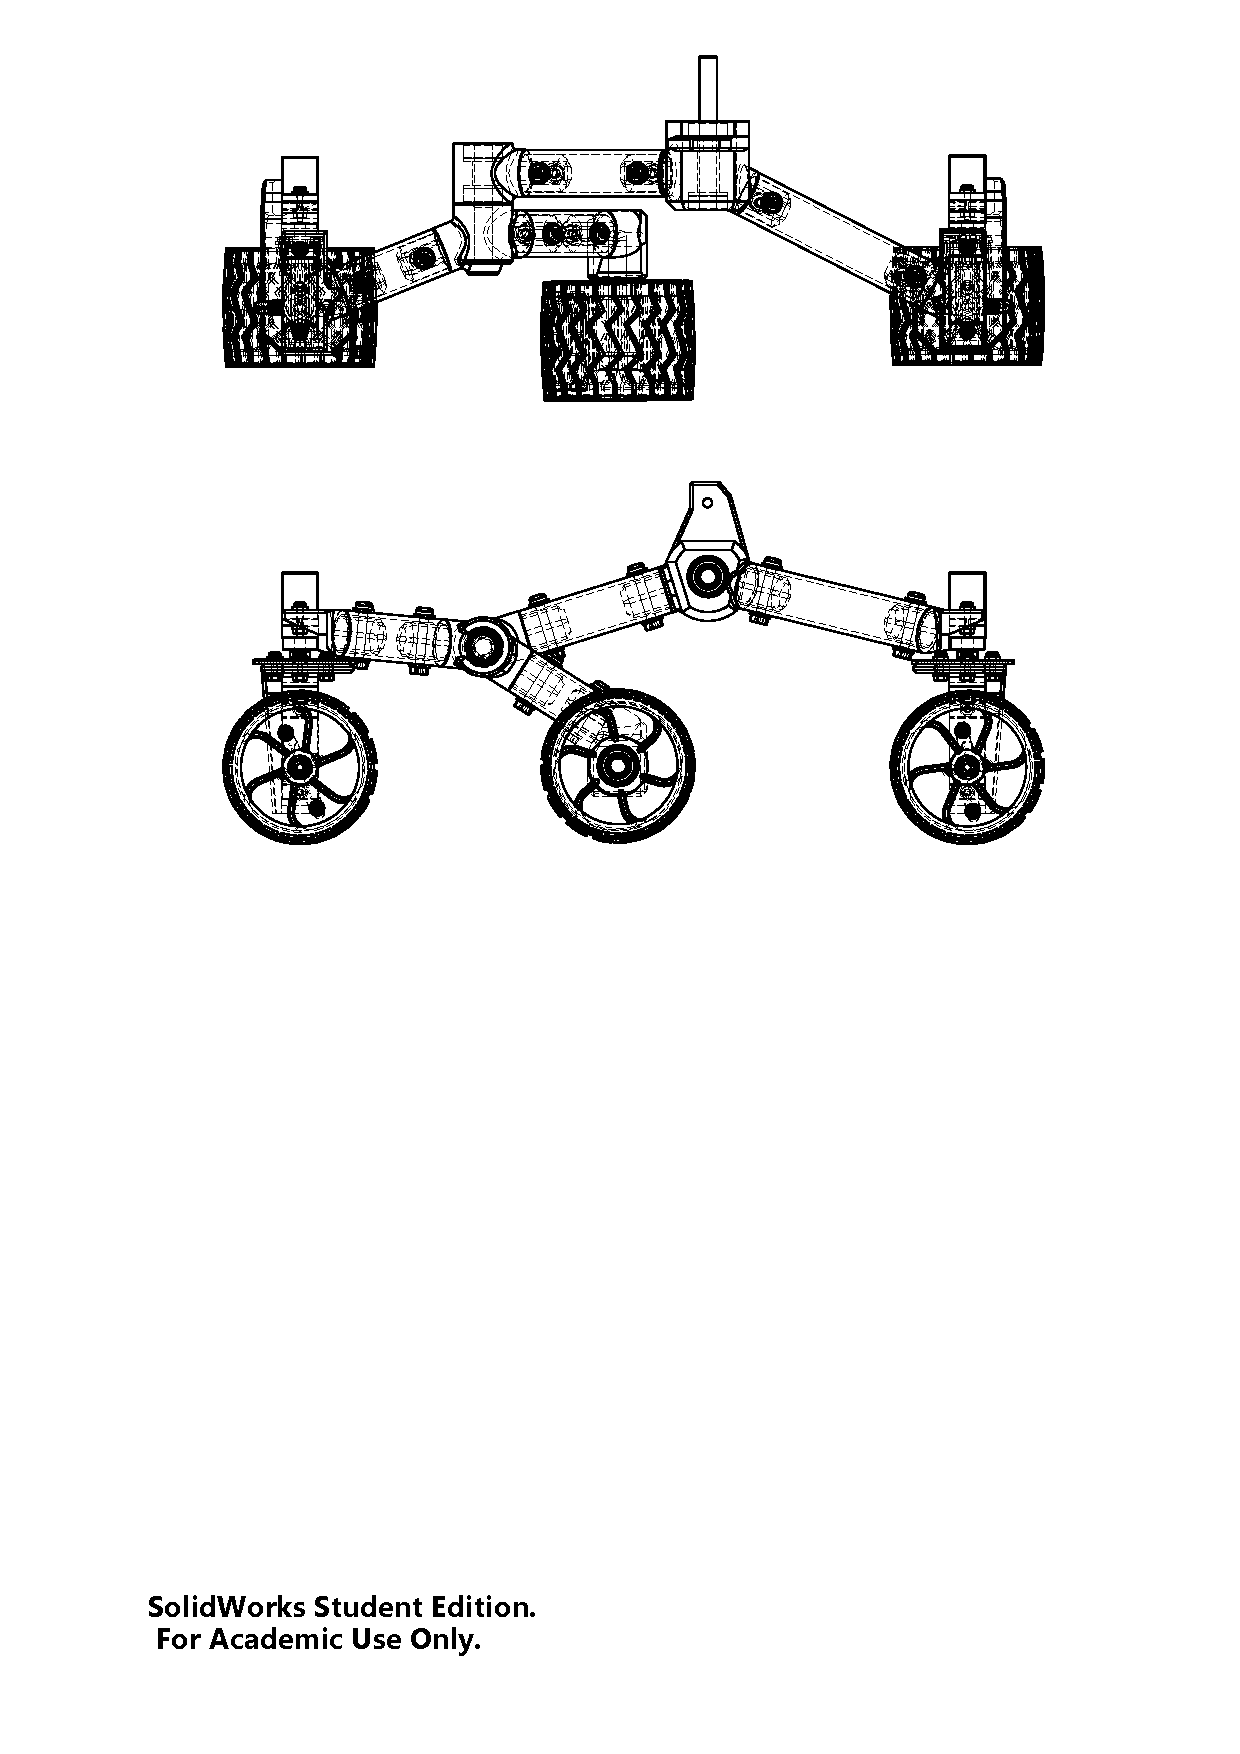
\includegraphics[clip, trim=2cm 15cm 2cm 1cm, width=0.9\linewidth]{figures/suspensionSub}
      }
      \qquad
      \subfloat[]{
        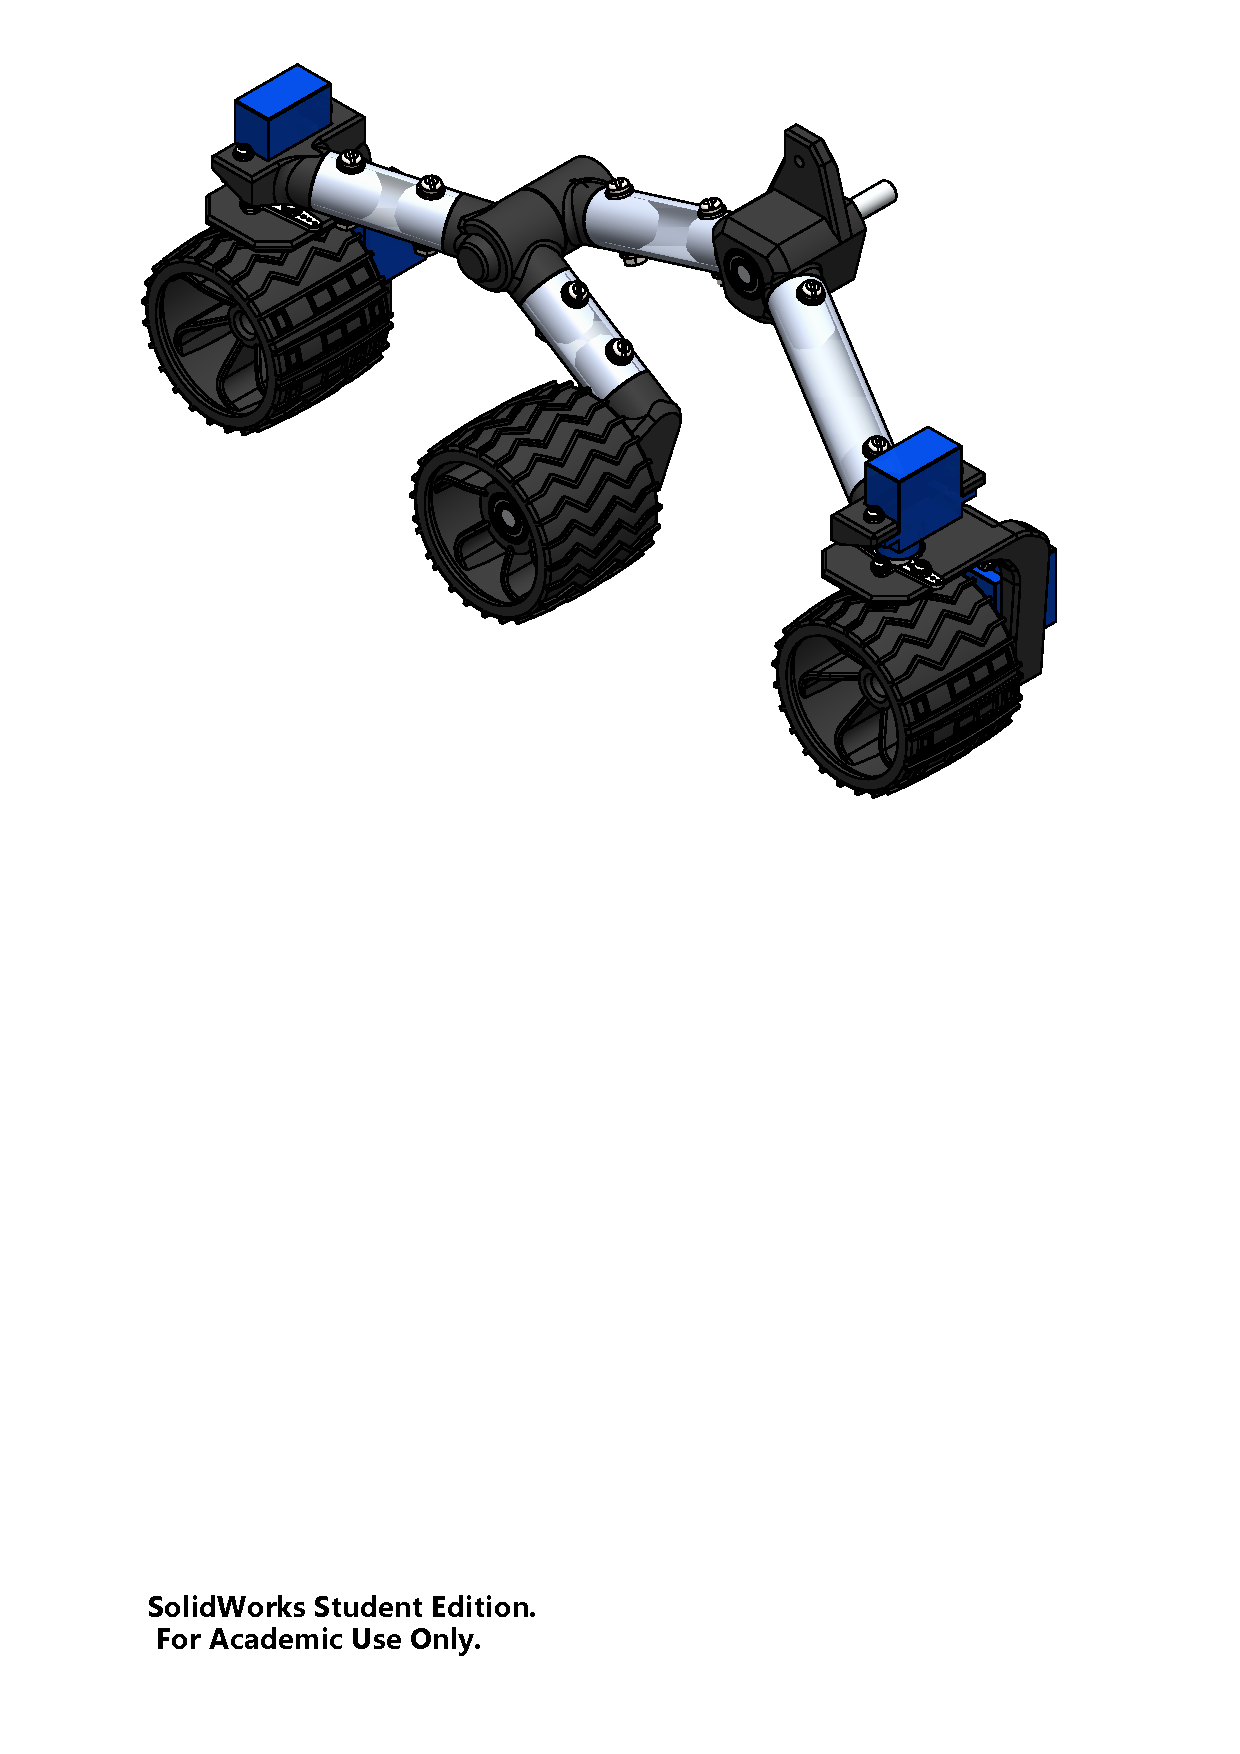
\includegraphics[clip, trim=2cm 15cm 2cm 1cm, width=0.7\linewidth]{figures/suspensionSub-iso}
      }
      \caption[Detailed drawings of the working, dynamic assembly one side of the suspension system]{Detailed drawings of the working, dynamic assembly one side of the suspension system}
      \label{fig:mechDesign-suspensionSubDetail}
      \end{figure}
      
      \begin{figure}[h!]
        \centering
        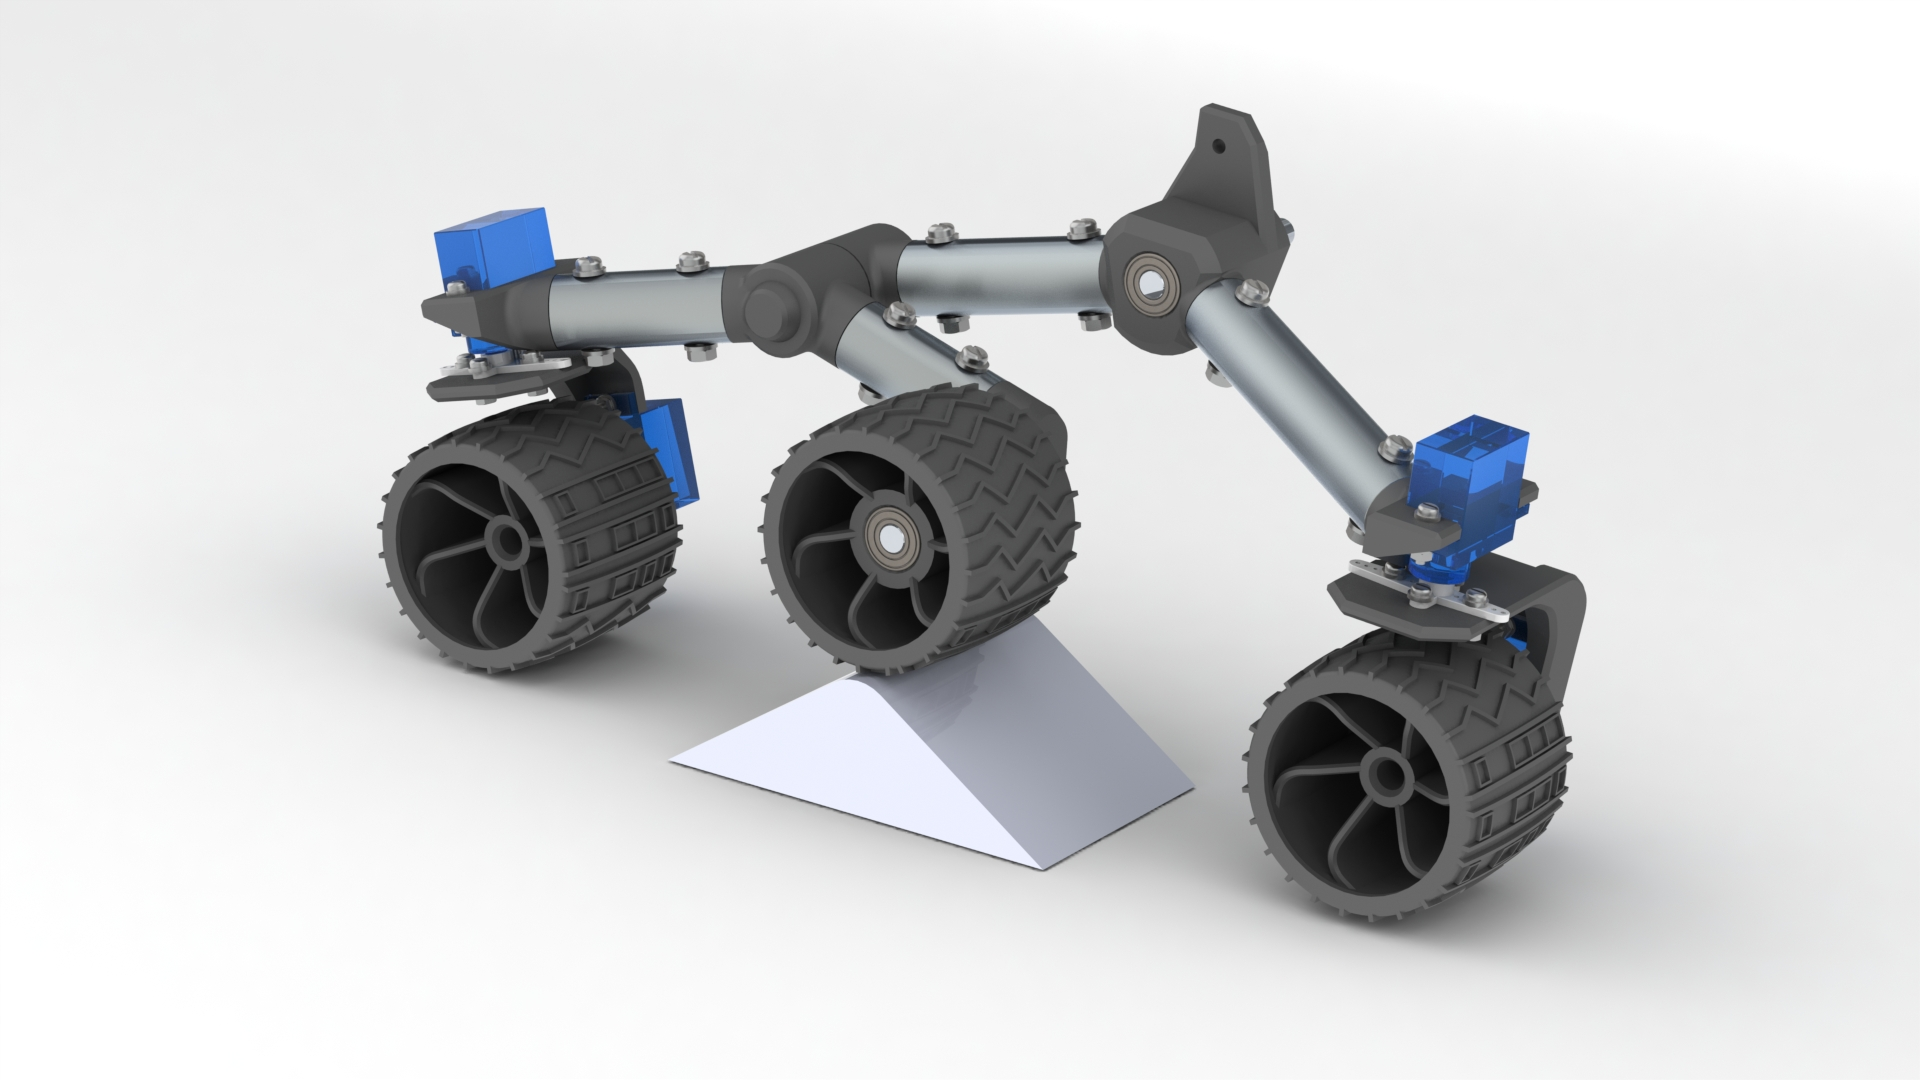
\includegraphics[width=1\linewidth]{figures/suspensionSub-obstacle}
        \caption[Render of one side of the suspension system navigating over an obstacle]{Render of one side of the suspension system navigating over an obstacle}
        \label{fig:mechDesign-suspensionSubObstacle}
      \end{figure}
      
    \subsubsection{Differential}
      Design of the differential involved a partially completed design of the body structure which contained details of the mounting points of the suspension system and thus the position of the connection point on the rocker joint, as well as the centre point of articulation of the differential bar as acquired from the reference model. The concept chosen for this subsystem included a 3D printed differential bar, printed hinges and threaded-bar (rods) attached to the hinges to link the differential to the rocker joint. The need for hinges was to provide the rods with the degrees of freedom required taking into the account the arced motions of an end of the differential bar in the $x$-$y$-plane and rocker joint in the $x$-$z$-plane. The articulation of the differential system and the resulting motion of the rods is depicted in Figure~\ref{fig:mechDesign-differentialMotion}, each of the two views showing two positions in the motion.
      
      \begin{figure}[h!]
      \centering
      \subfloat[Top view\label{fig:mechDesign-differentialMotion-a}]{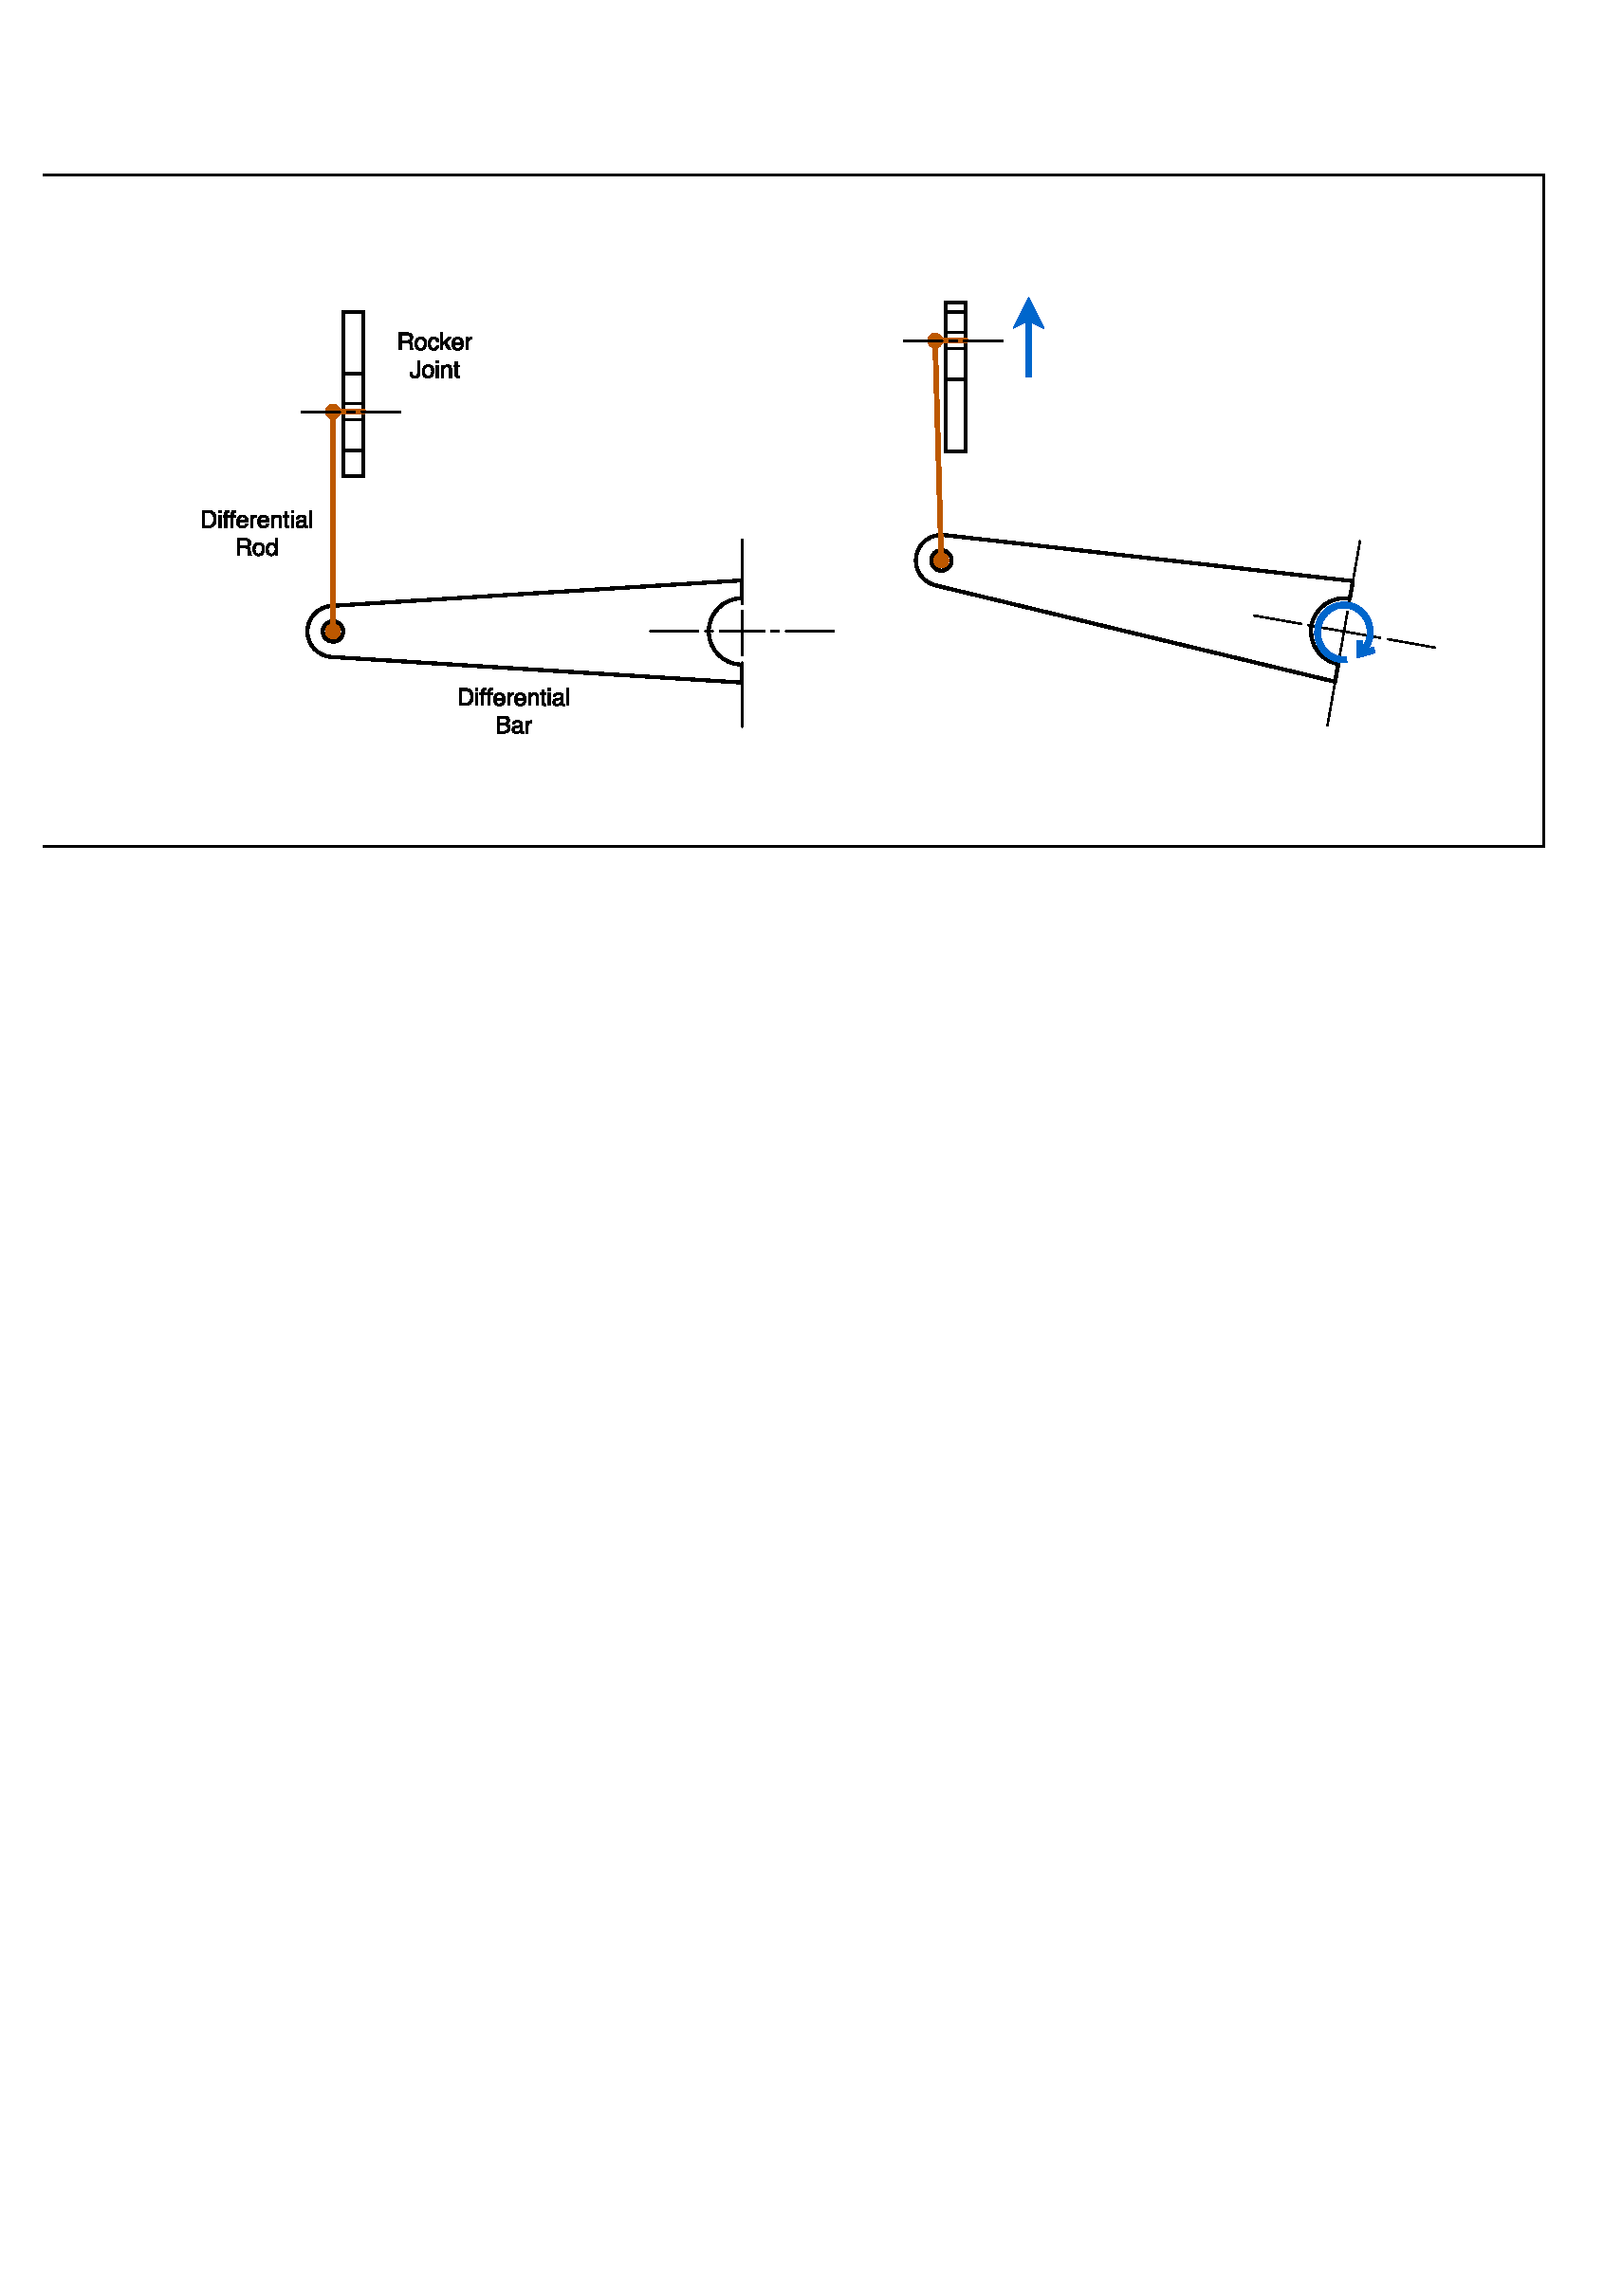
\includegraphics[clip, trim=2cm 26cm 2cm 4cm, width=0.9\linewidth]{figures/mechDesign-differentialMotionTop.pdf}}
      \qquad
      \subfloat[Side view]{
        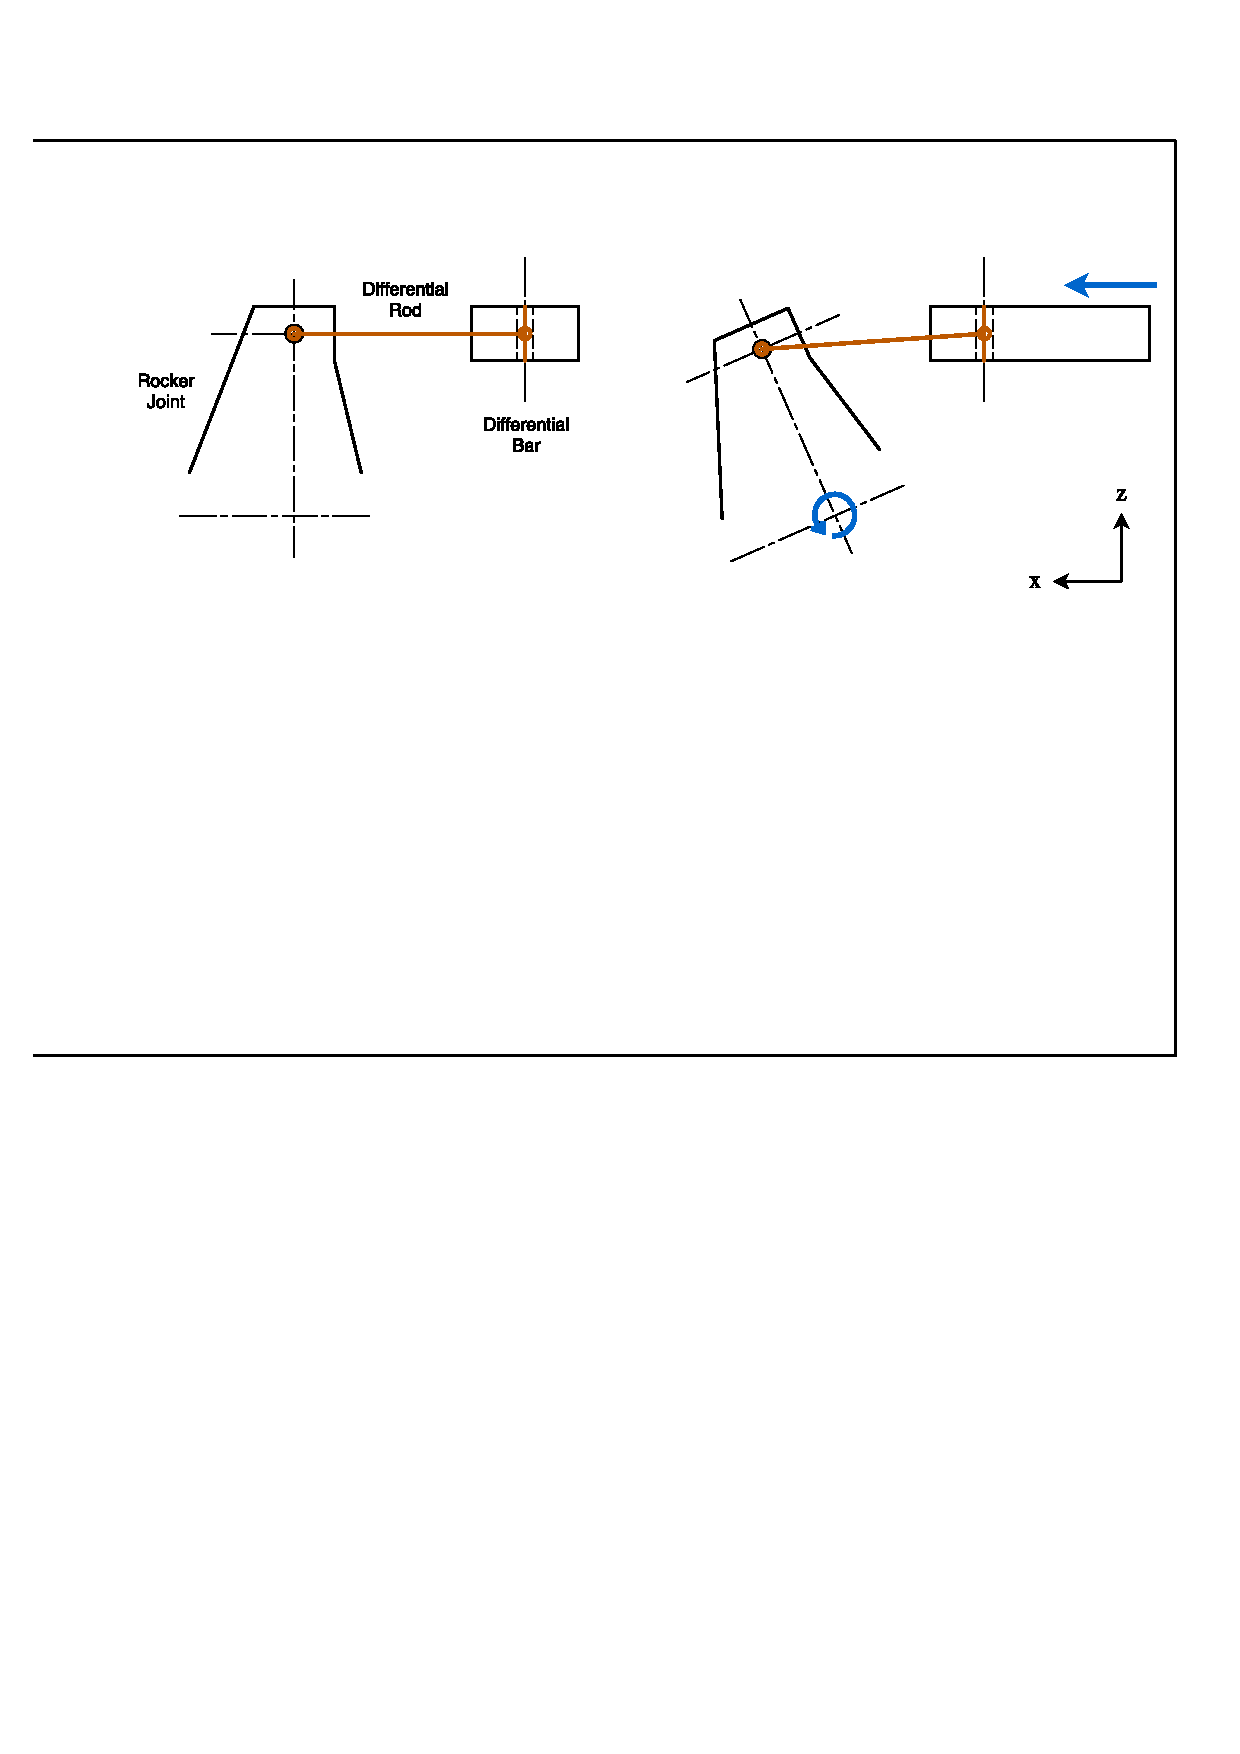
\includegraphics[clip, trim=2cm 26cm 2cm 4cm, width=0.9\linewidth]{figures/mechDesign-differentialMotionSide.pdf}
      }
      \caption[Diagram showing the motion of the differential and the resulting motion of the differential rod]{Diagram showing the motion of the differential and the resulting motion of the differential rod}
      \label{fig:mechDesign-differentialMotion}
      \end{figure}
      
      % TODO: Add axes to the above figure
      
      \subheading{Differential Bar}\\\\
        The design of the differential bar stemmed from the partially completed rover deck, specifically with respect to the width of the body and therefore the span of the rocker joints' differential connection points. The bar took on the tapered shape as on \textit{Curiosity} with the wider section in the centre and narrower ends. A hole was added for the addition of a bearing in the centre of the bar and holes for the hinges added to the ends. The bearing was to be mounted to a short shaft which was to be fixed into the deck of the rover. Figure~\ref{fig:mechDesign-differentialBarDetail} shows the detail of the differential bar.
        
        \begin{figure}[h!]
        \centering
        \subfloat[]{
          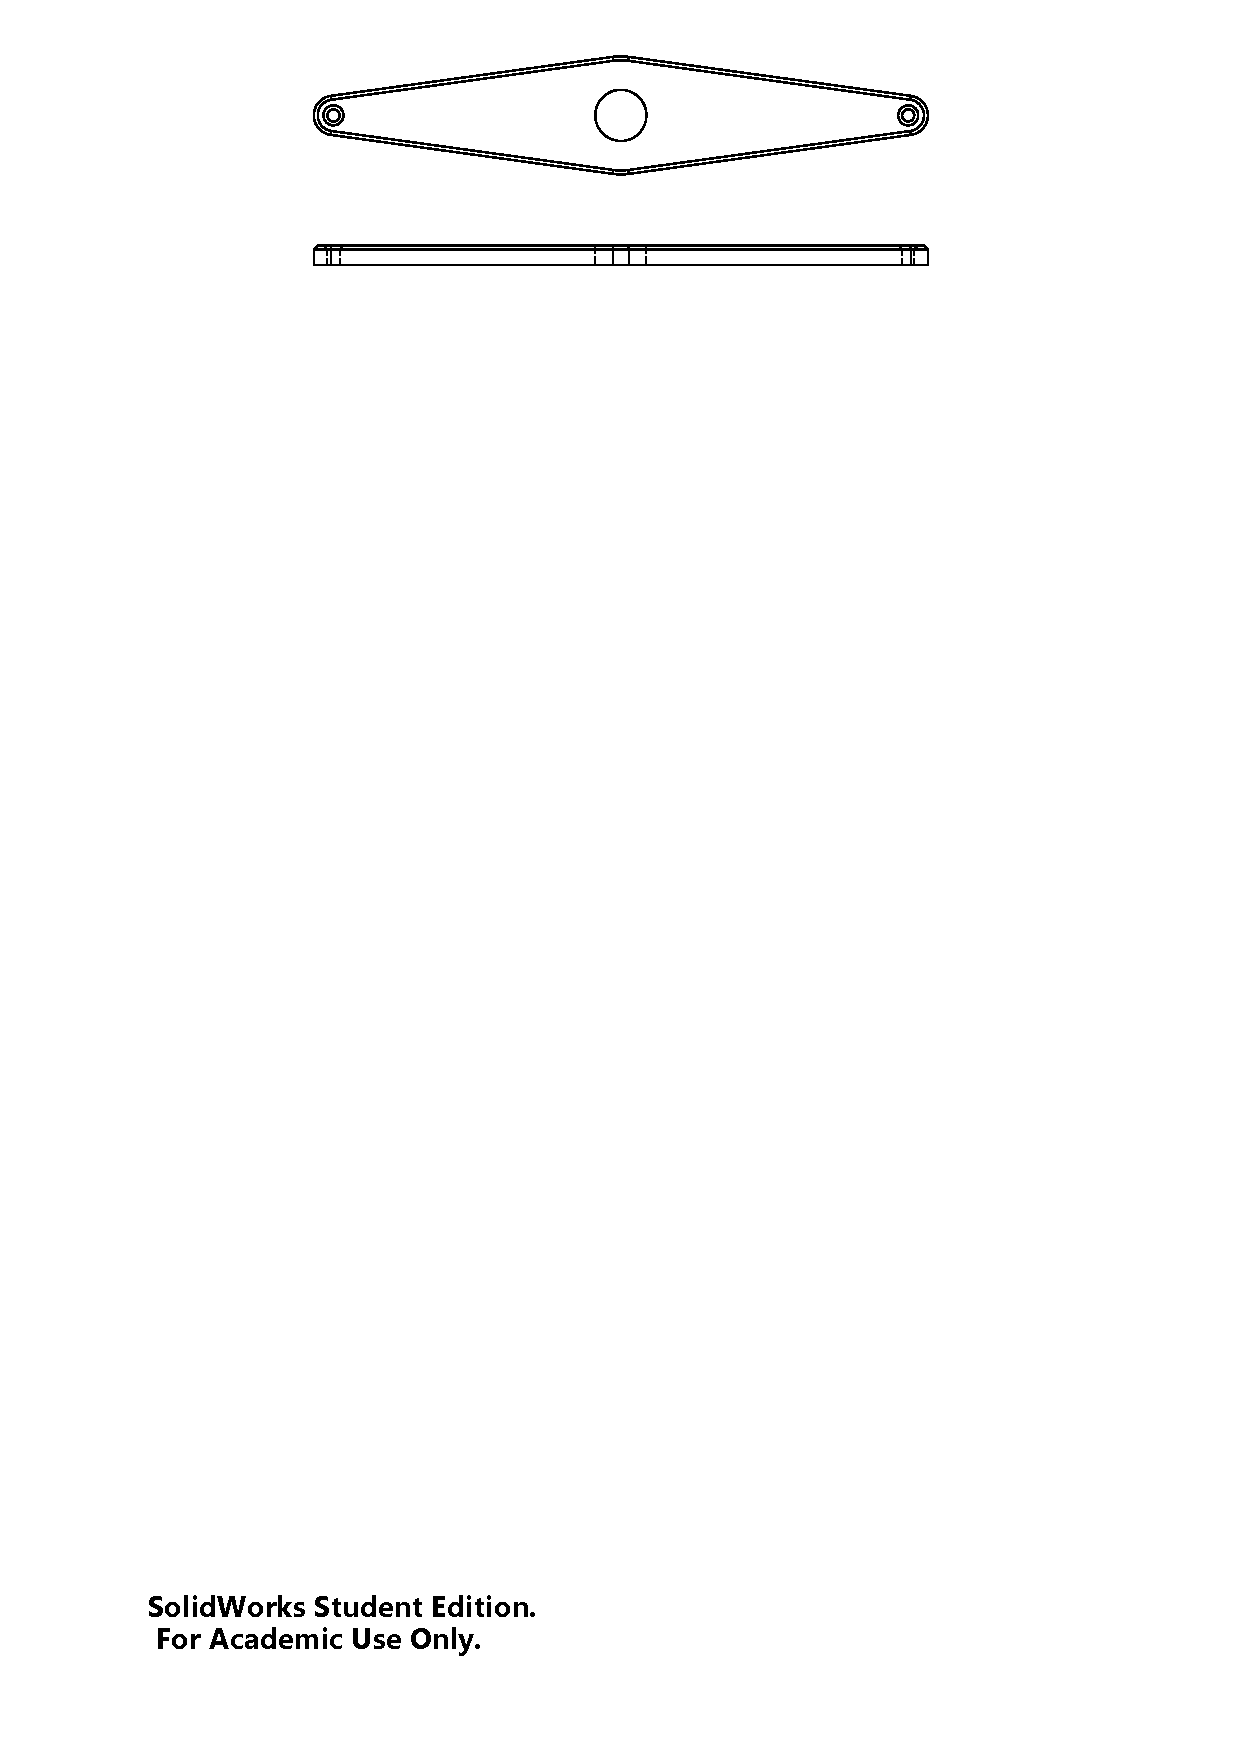
\includegraphics[clip, trim=5cm 24cm 5cm 0cm, width=0.5\linewidth]{figures/differential-bar}
        }%
        \subfloat[]{
          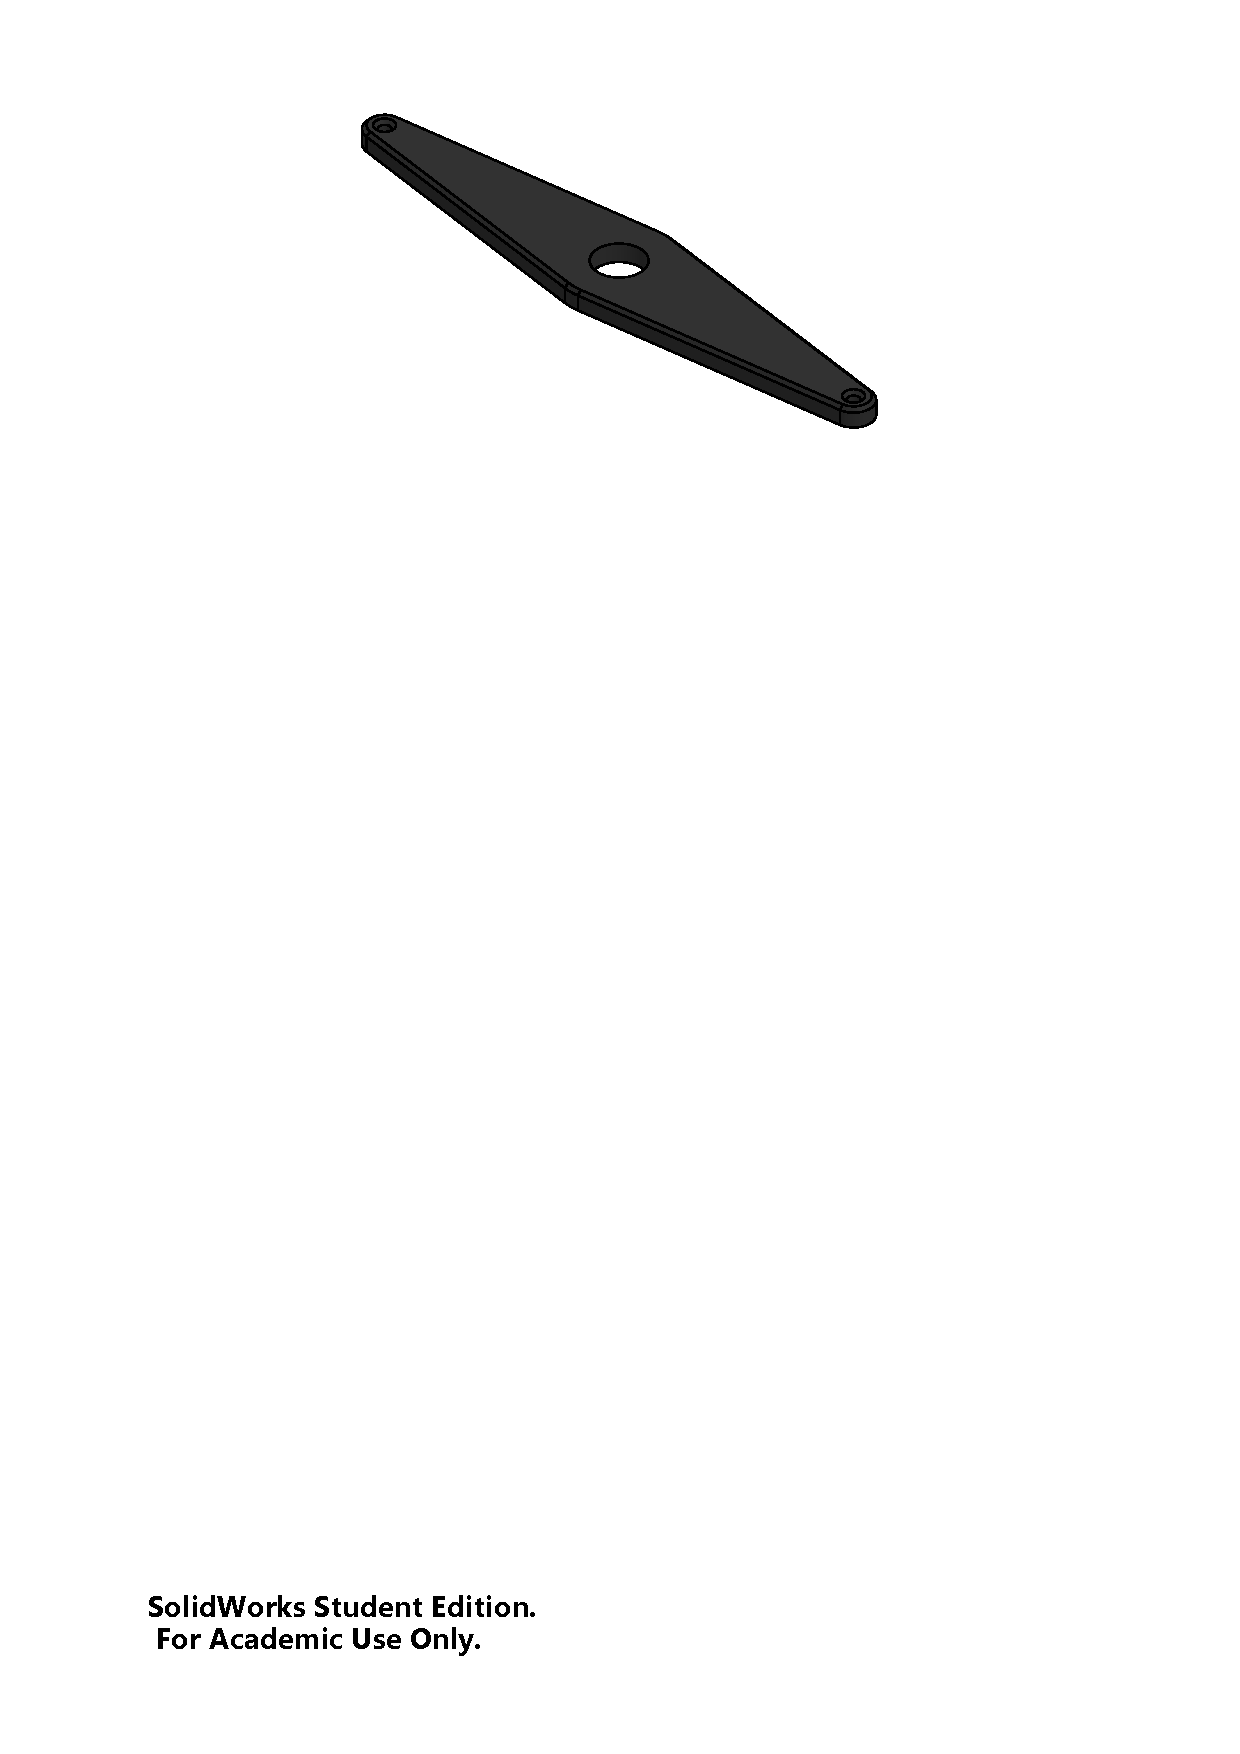
\includegraphics[clip, trim=3cm 21cm 3cm 1cm, width=0.49\linewidth]{figures/differential-bar-iso}
        }
        \caption[Detailed drawings of the differential bar component in the differential system]{Detailed drawings of the differential bar component in the differential system}
        \label{fig:mechDesign-differentialBarDetail}
        \end{figure}
        
        
      \subheading{Hinges}\\\\
        Hinges were designed for each end of the rods, one end on the rocker joint side and the other for the differential bar. The hinges allowed rotation about specific axes, the $y$- and $z$-axes on the bar side and the $y$-axis on the joint side. Figure~\subref*{fig:mechDesign-differentialMotion-a} demonstrates that the bar also rotates about the $z$-axis which would require the hinge at the rocker joint to allow for this motion. However, this was not included in the design after confirming through calculation that the amount by which the bar would have rotated in this direction at the maximum angle of articulation of the differential bar ($\approx9^\circ$) did not justify the resulting added complexity in the hinge design.
        
        The single axis hinge on the rocker joint side amounted to a right-angled piece with a hole in one of the flat sections for fastening it to the rocker joint and another hole on the other flat section for fastening of the threaded-bar rod component. Slotted bolts and nuts were used for the joint hole, with washers between the joint and the hinge part to minimise the friction between the parts despite a small degree of motion that would be effected on this coupling. For the rod, two nuts on either side of the piece were used to fix the threaded-bar.
        
        The two-axis hinge on the differential-bar end included a part with two tabs with holes, one above and one below the end of the bar and a flat section extending perpendicular to the axis made between the two tab-holes. The additional section included a third hole to allow attachment of the second part used for mounting the rod. The second component included a blind hole into which the rod could be place and a cutout halfway down the length of the hole to allow for a nut to be pushed into place. This meant that the rod could be screwed into the piece, the purpose of which included easy assembly and breakdown if required as well as allowing the extension of the rod to be adjusted. Therefore, the differential system could be adjusted to balance the rover body about the rocker joint pivot points.
        
        Detailed drawings of both hinge assemblies can be seen in Figures~\ref{fig:mechDesign-singleAxisHingeDetail} and \ref{fig:mechDesign-twoAxisHingeDetail}.
        
        \begin{figure}[h!]
        \centering
        \subfloat[]{
          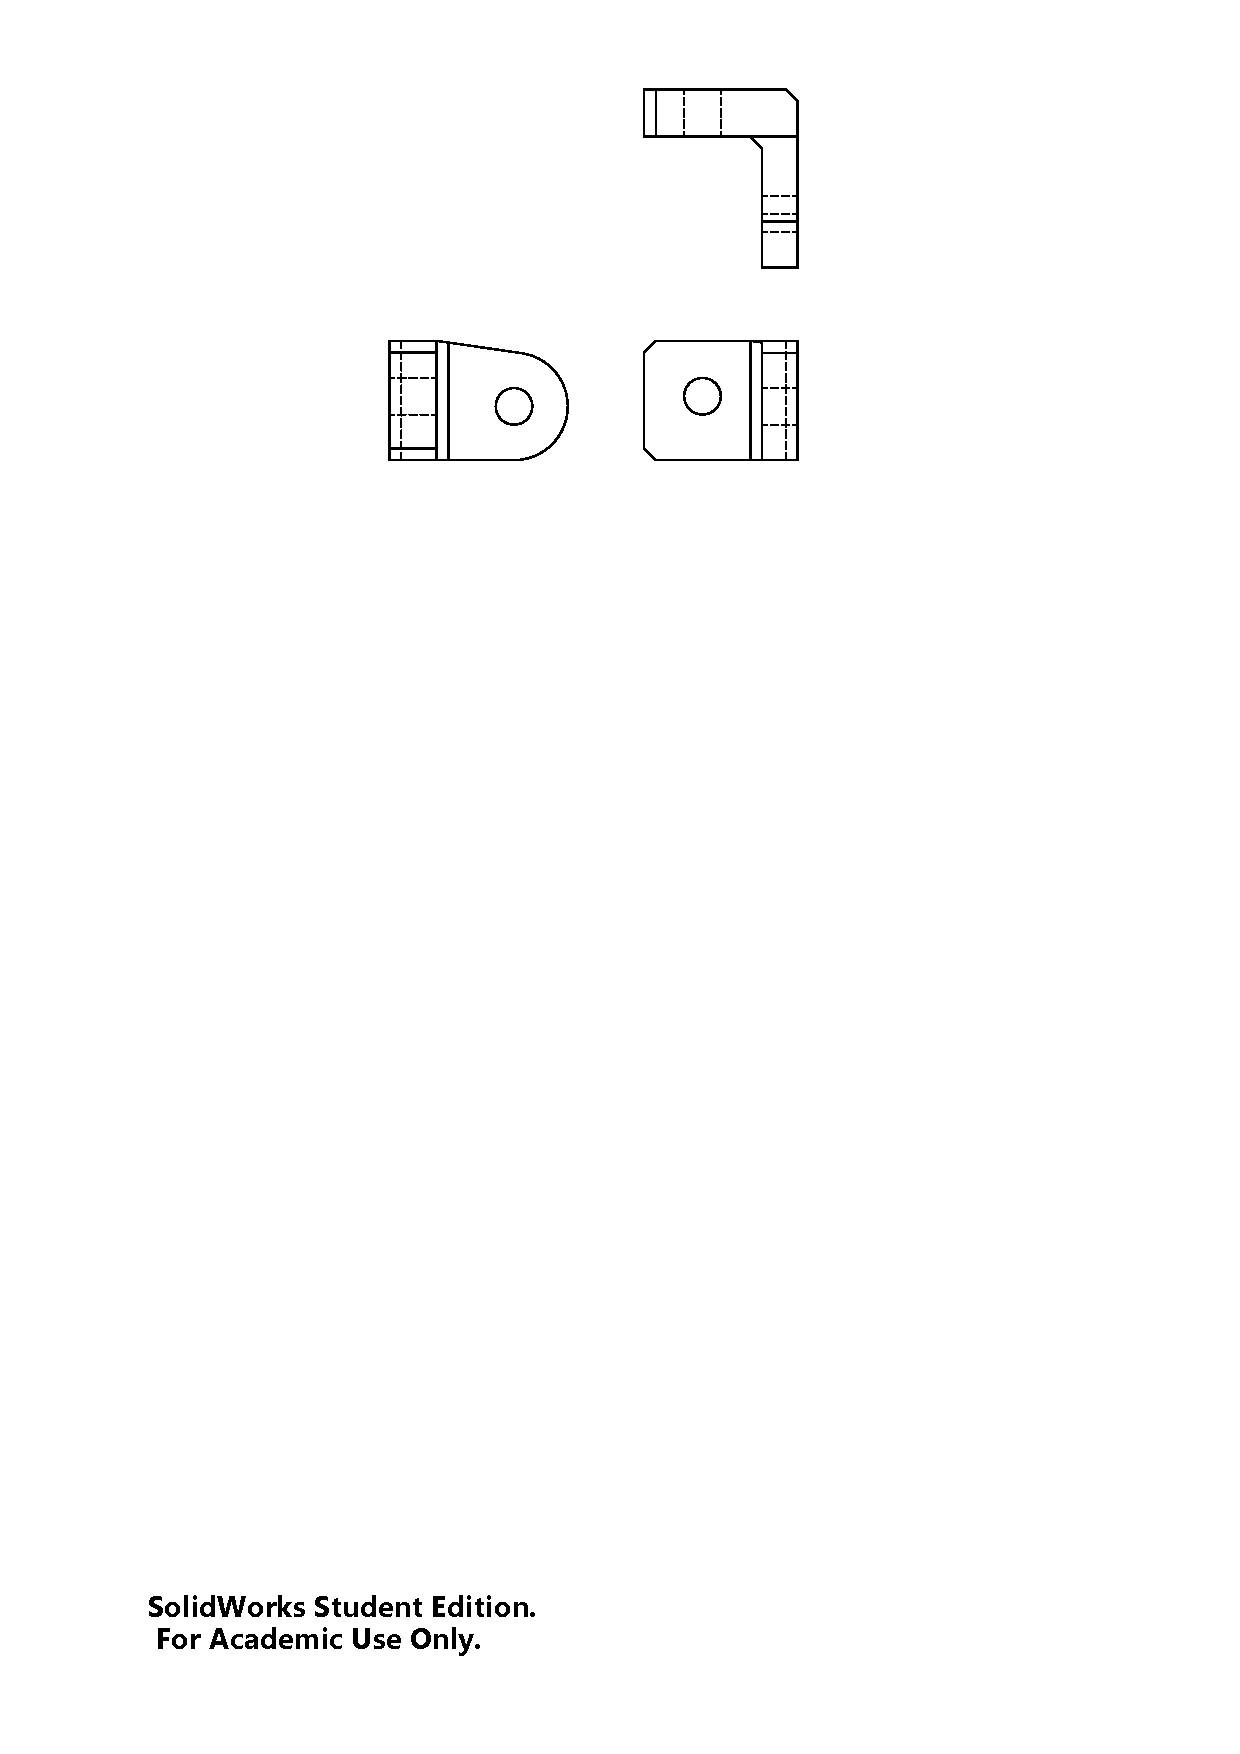
\includegraphics[clip, trim=9cm 24cm 6cm 0cm, width=0.4\linewidth]{figures/rod-hing-jointSide}
        }
        \qquad
        \subfloat[]{
          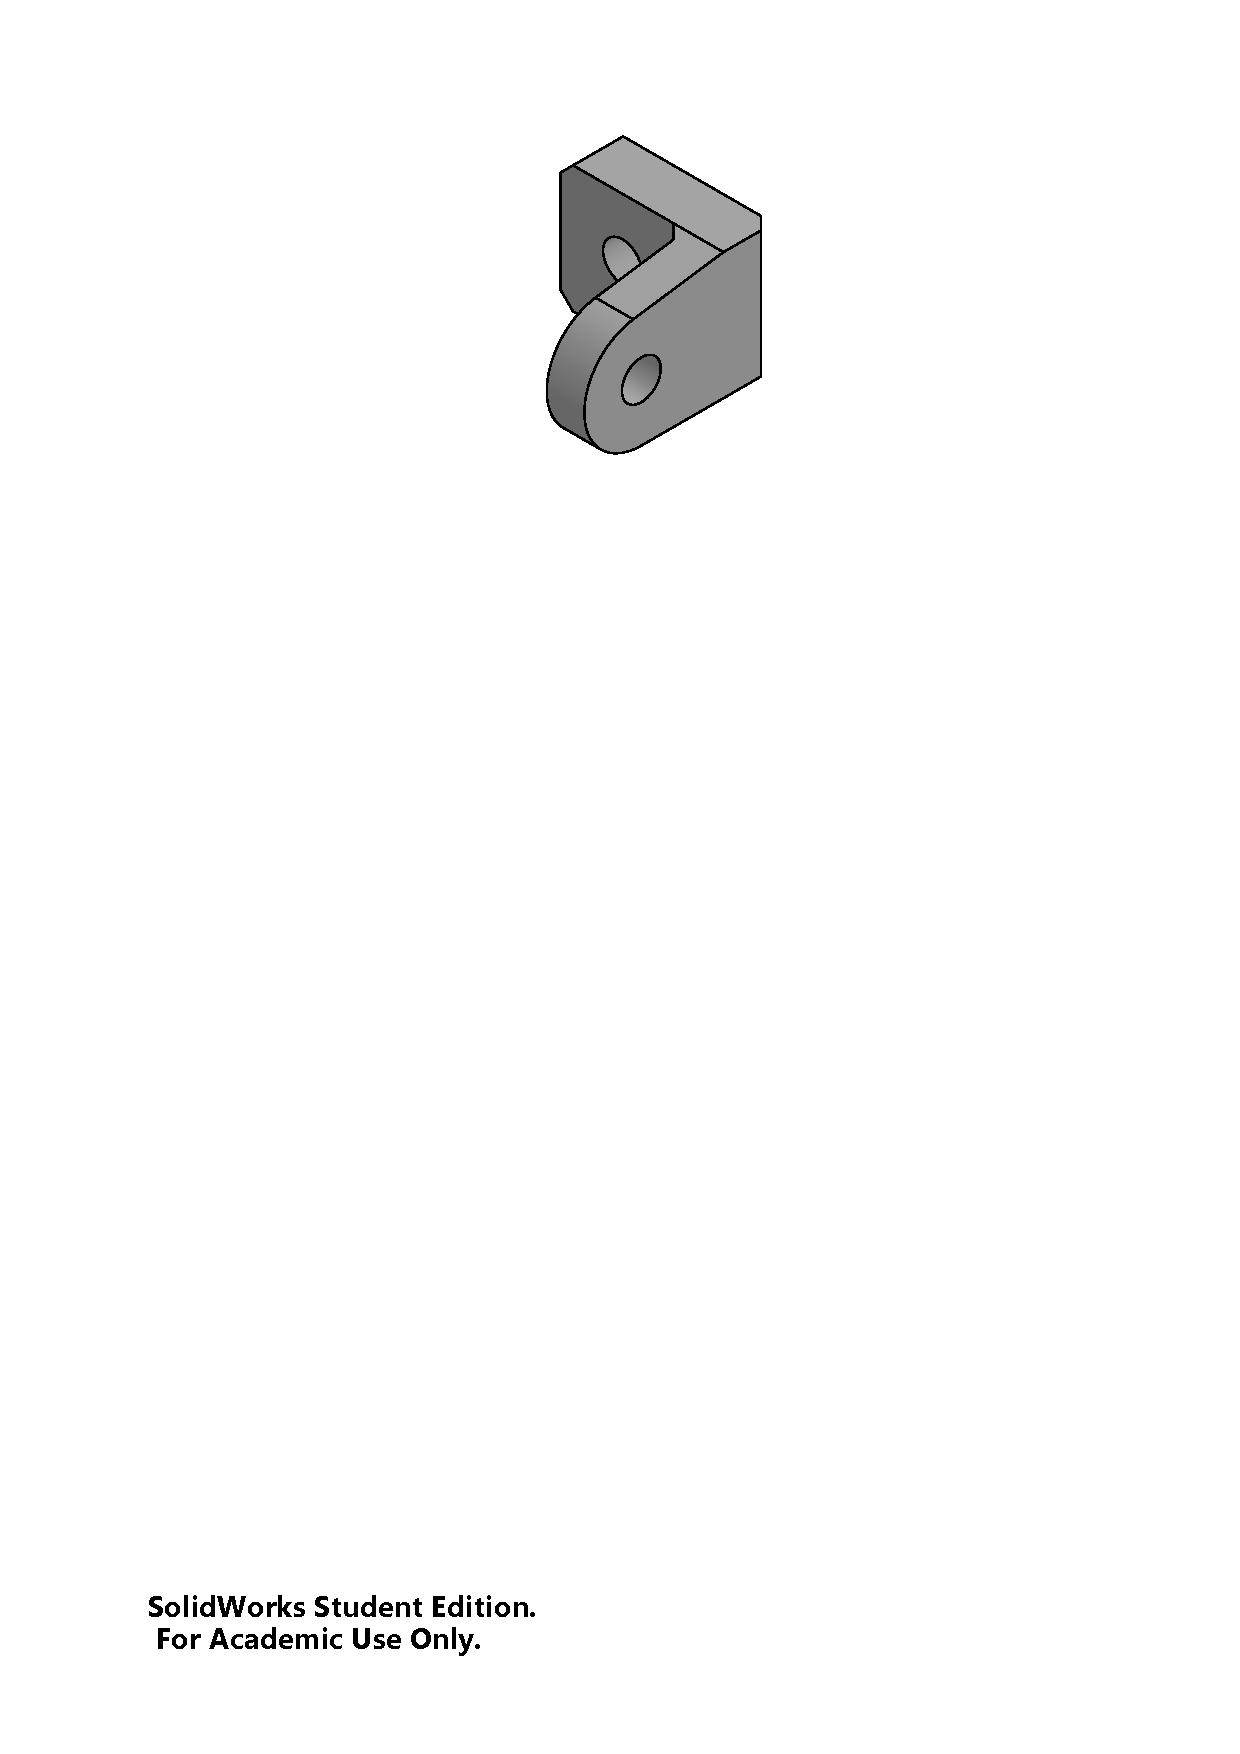
\includegraphics[clip, trim=5cm 20cm 5cm 1cm, width=0.4\linewidth]{figures/rod-hing-jointSide-iso}
        }
        \caption[Detailed drawings of the single-axis hinge component in the differential system]{Detailed drawings of the single-axis hinge component in the differential system}
        \label{fig:mechDesign-singleAxisHingeDetail}
        \end{figure}
        
        \begin{figure}[h!]
        \centering
        \subfloat[]{
          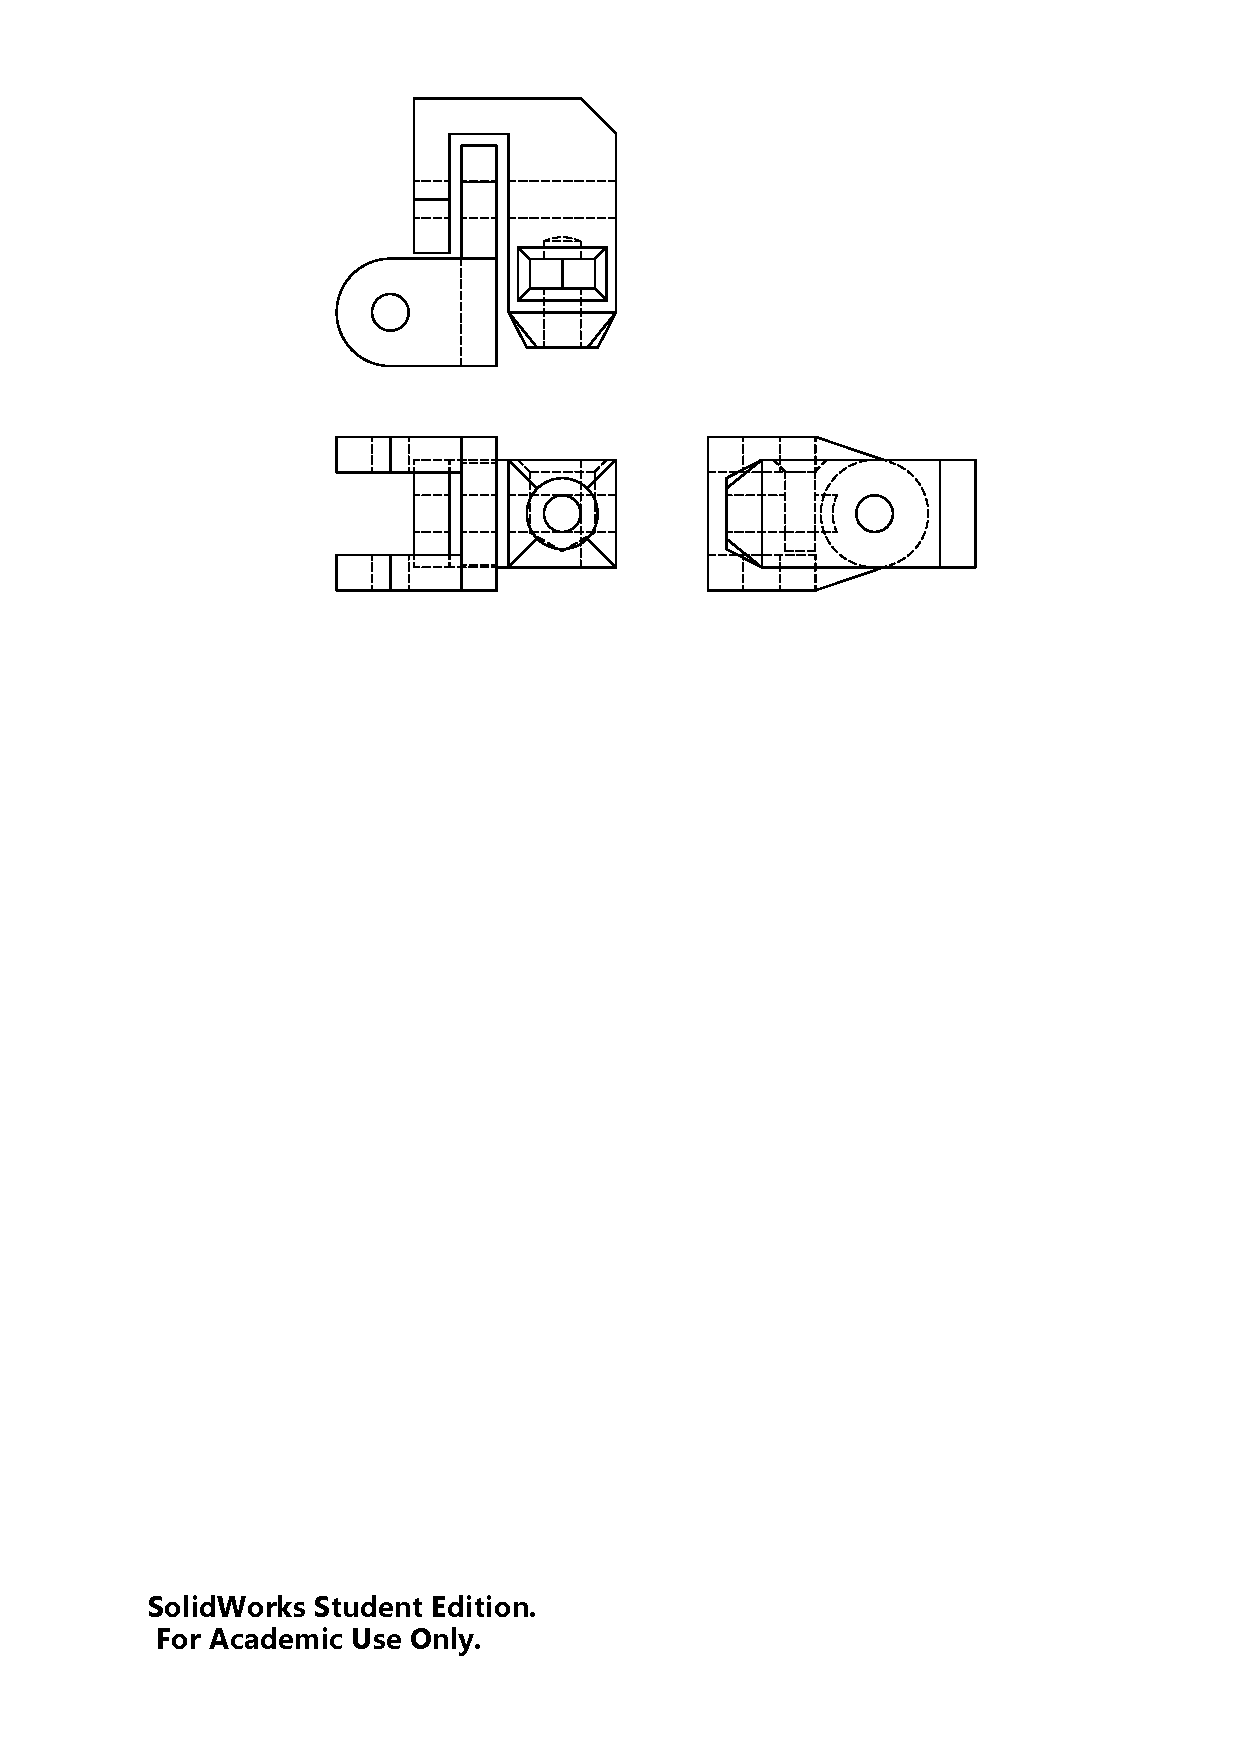
\includegraphics[clip, trim=5cm 18cm 4cm 0cm, width=0.44\linewidth]{figures/two-axis-hinge}
        }%
        \subfloat[]{
          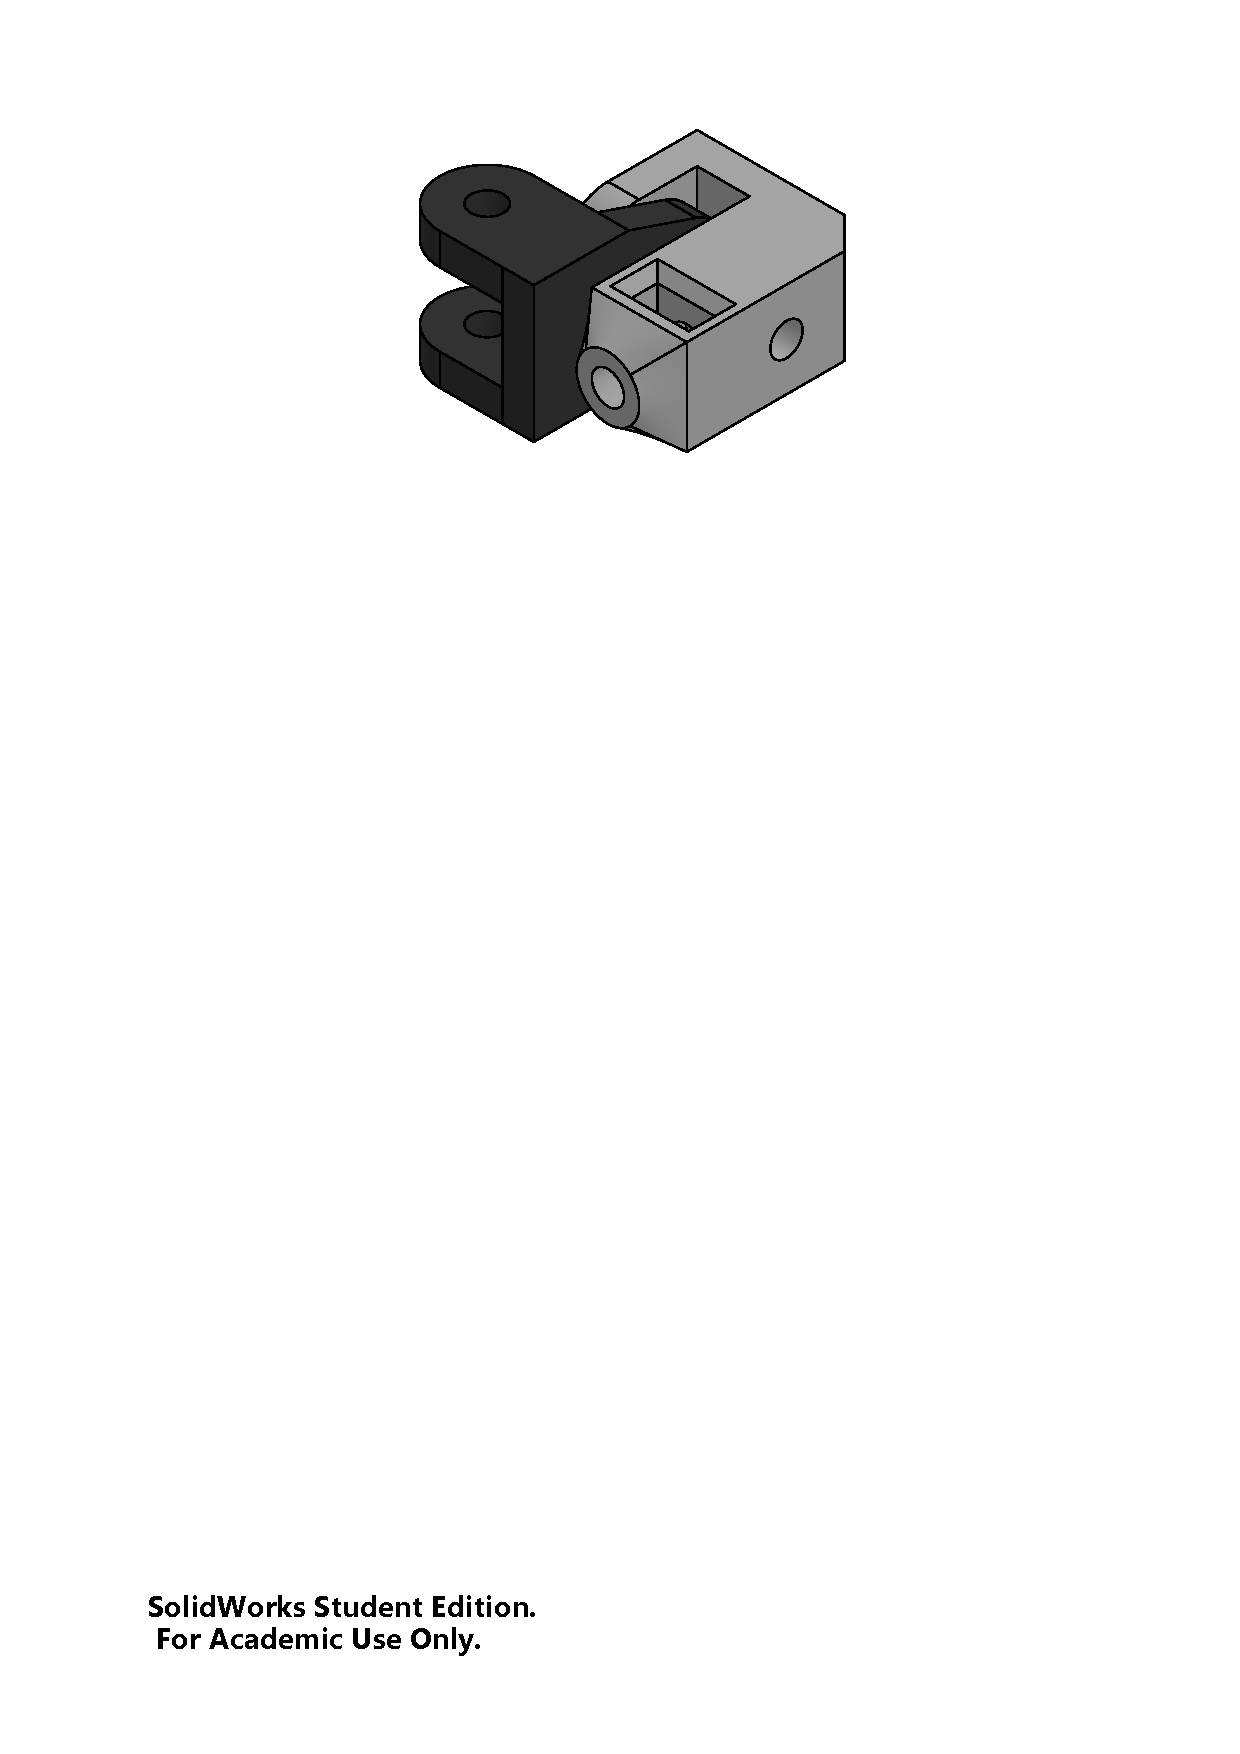
\includegraphics[clip, trim=3cm 19cm 3cm 1cm, width=0.55\linewidth]{figures/two-axis-hinge-iso}
        }
        \caption[Detailed drawings of the two-axis hinge component in the differential system (without fasteners)]{Detailed drawings of the two-axis hinge component in the differential system (without fasteners)}
        \label{fig:mechDesign-twoAxisHingeDetail}
        \end{figure}
        
        It must be noted that other hinge techniques were considered also for this subsystem, one of which included a ball and ring-socket joint which would have provided the required axes of rotation in a single coupling (for each end). The idea was not used for the design due to unavailability of the joints, particularly of the size required. The hinge technique was simpler in design and leant itself well to the chosen manufacture method.
        
      \subheading{Final Sub-assembly}\\\\
        Figure~\ref{fig:mechDesign-differentialSubDetail} shows detail of the differential sub-assembly as generated in the CAD package used and which was analysed for interferences and functional integrity.
        
        \begin{figure}[h!]
        \centering
        \subfloat[\label{fig:mechDesign-differentialSubDetail-a}]{
          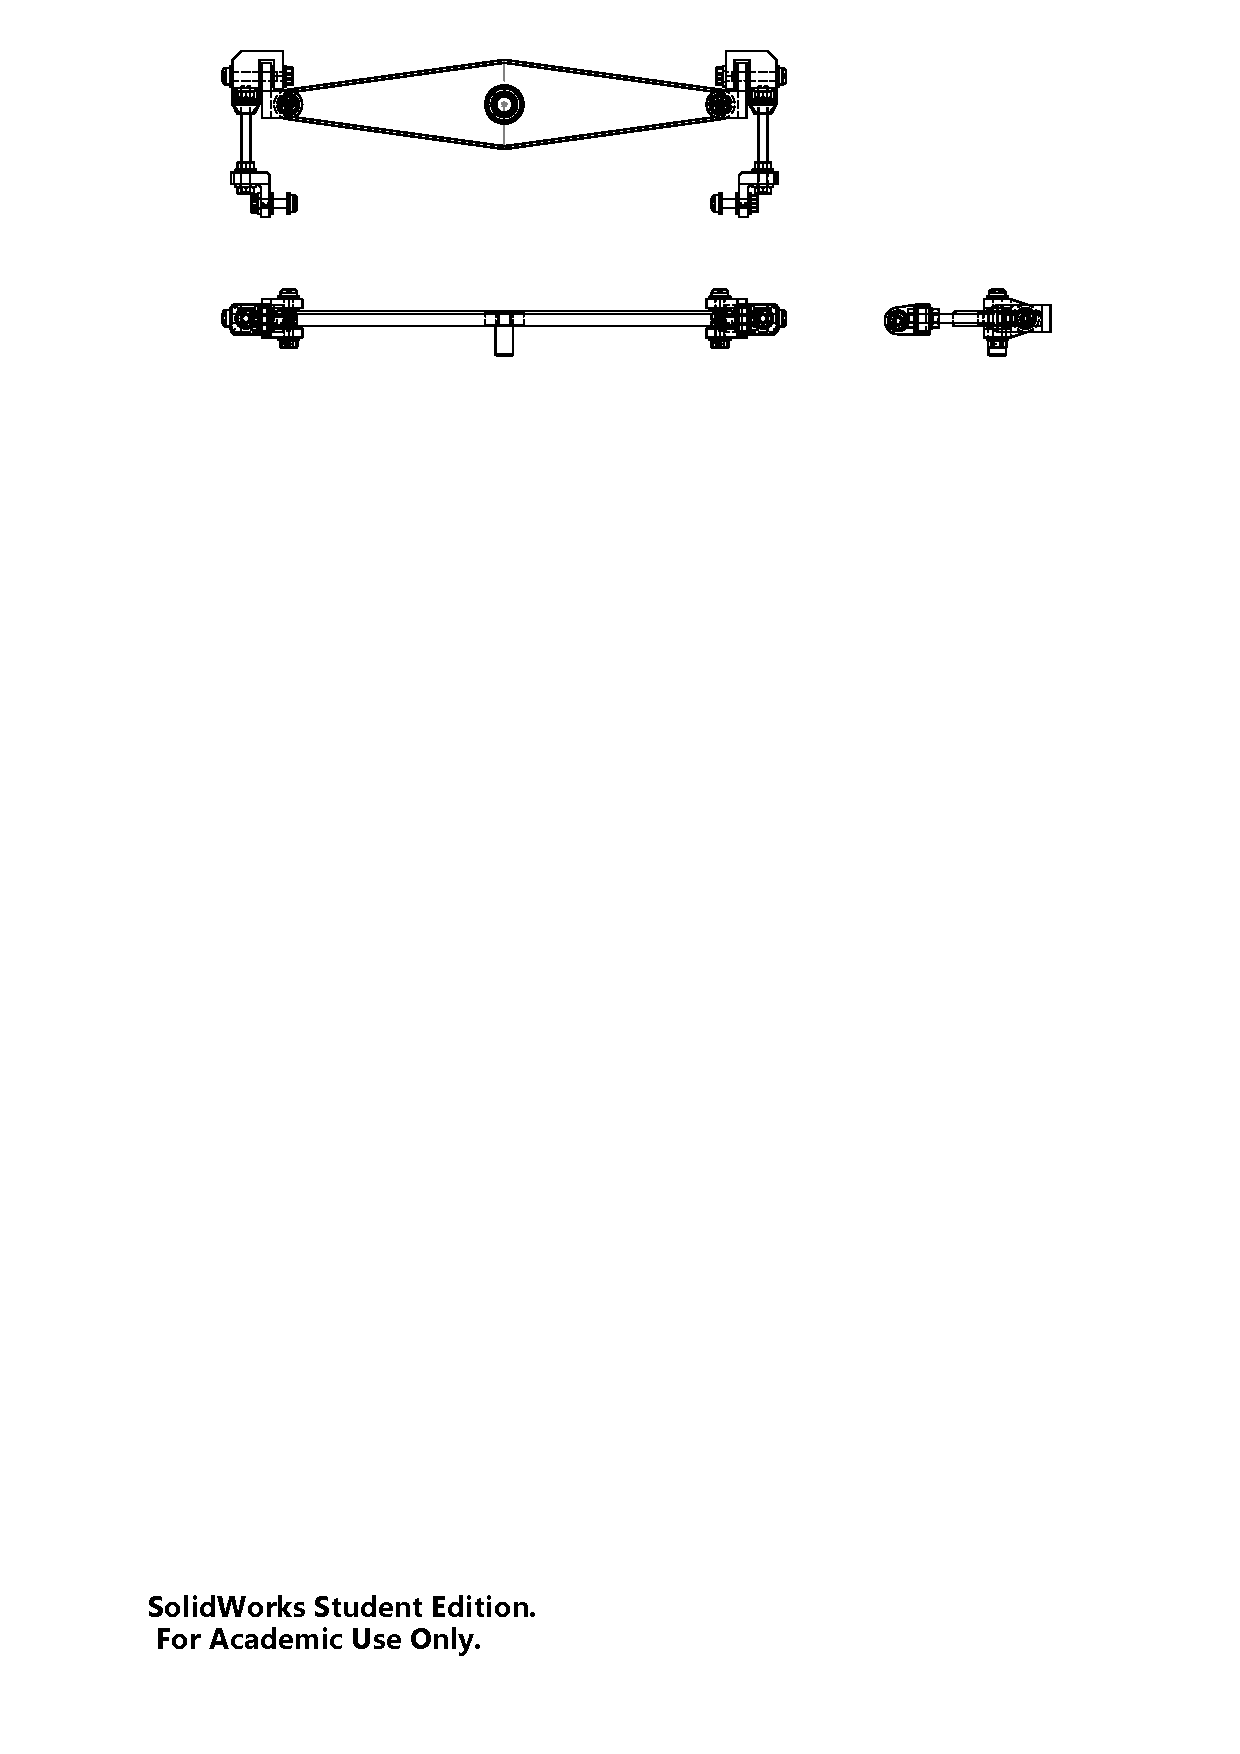
\includegraphics[clip, trim=3cm 22cm 3cm 0cm, width=1\linewidth]{figures/diff-sub}
        }
        \qquad
        \subfloat[\label{fig:mechDesign-differentialSubDetail-b}]{
          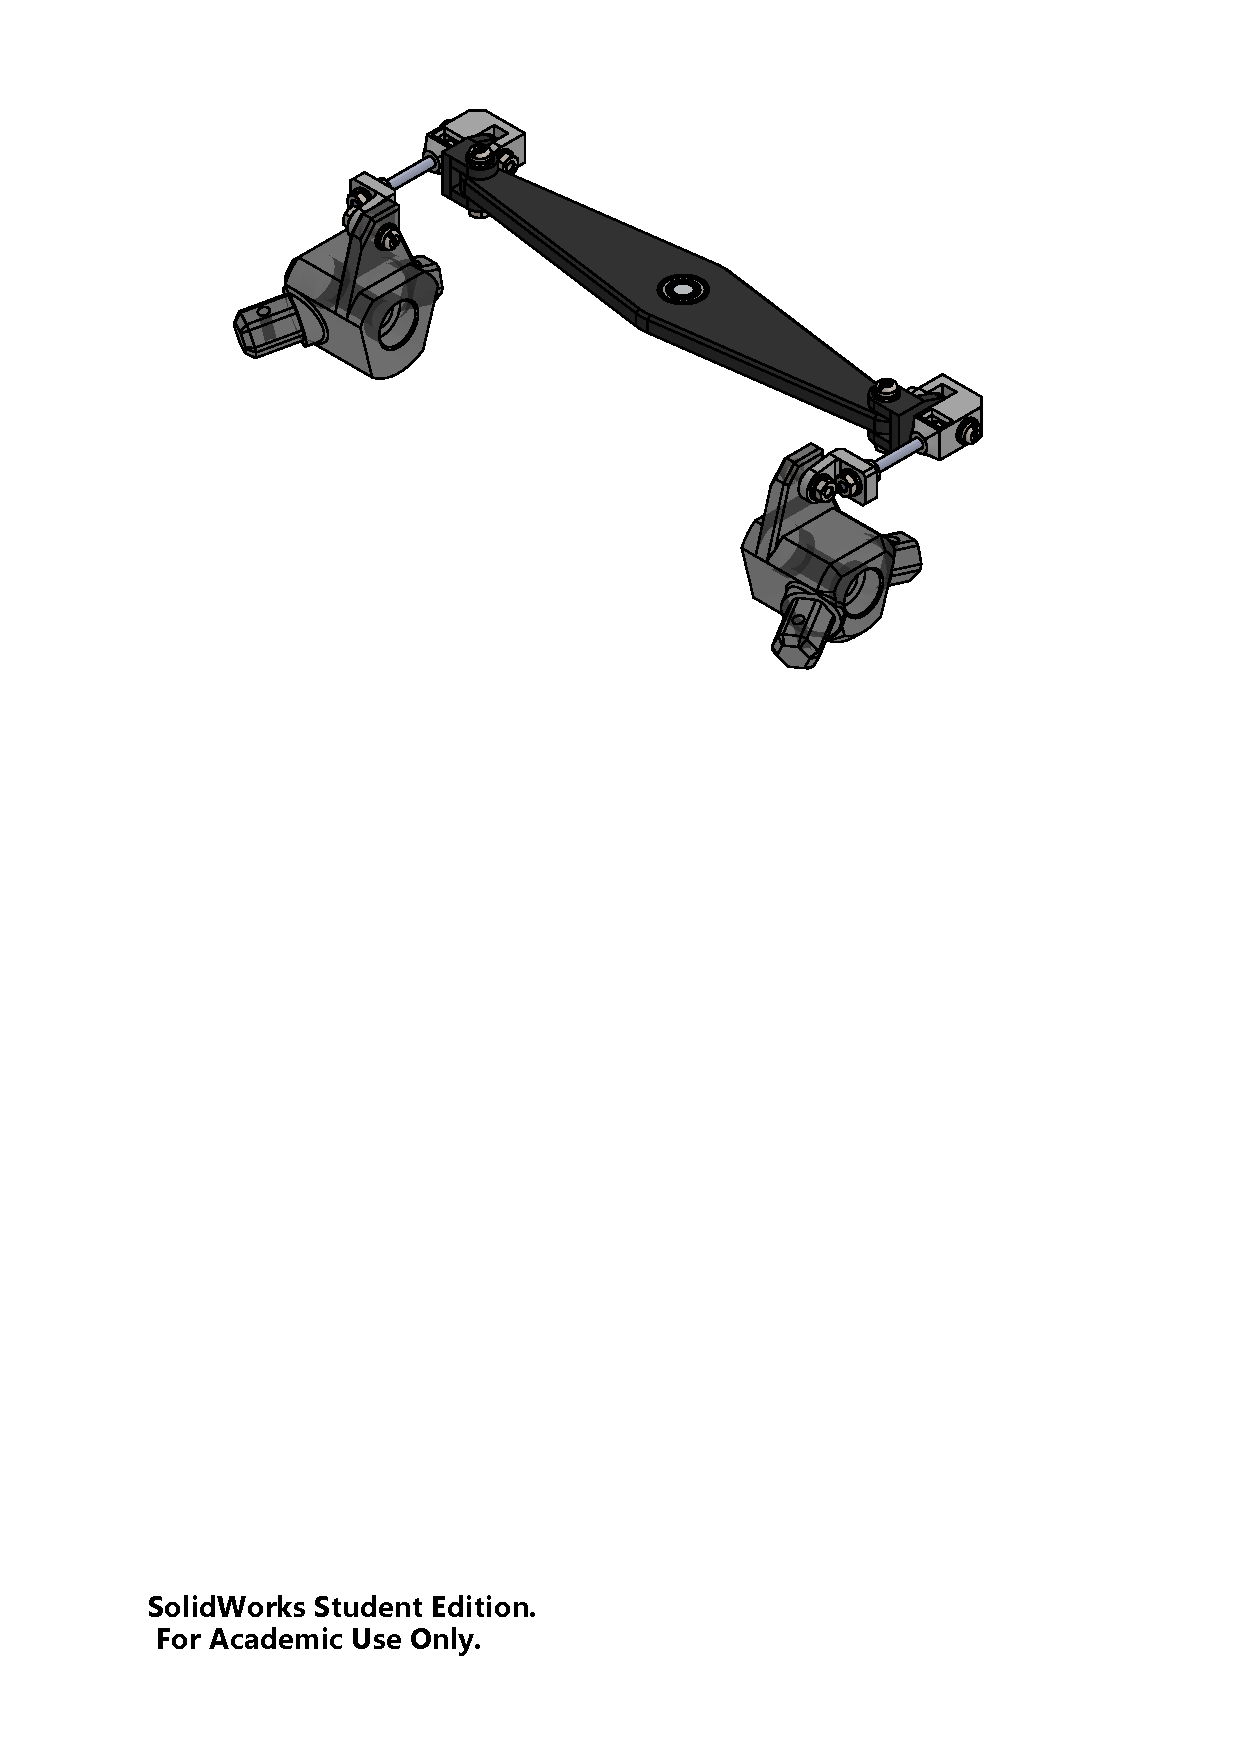
\includegraphics[clip, trim=4cm 17cm 4cm 1cm, width=0.7\linewidth]{figures/diff-sub-iso}
        }
        \caption[Detailed drawings of the working, dynamic assembly of the differential system]{Detailed drawings of the working, dynamic assembly of the differential system (included in the isometric view in \protect\subref{fig:mechDesign-differentialSubDetail-b} are the rocker joints as part of the suspension system)}
        \label{fig:mechDesign-differentialSubDetail}
        \end{figure}
        
              
    \subsubsection{Head and Neck}
      It was decided during the conceptual design phase that both the neck and the head assembly were to be 3D printed and mounted to the top of the rover deck. Since there were two axes of rotation of the head required, as well as at least one piece to facilitate mounting the assembly, three separate components in total were required (a minimum). The assembly also aimed to minimise the amount of movement that components that facilitated mounting of the servos were subjected to for friendlier cable routing. At the same time, the ease of 3D printing such an assembly had an effect on the approach taken when designing the structure and configuration of the components as well as the components themselves. As a result, the configuration designed consisted of a static mount piece, a middle section, referred to as the neck, which allowed mounting of both servos for the two axes of rotation, and a head sub-assembly to mount the camera and the ultrasonic sensor.
      
      \subheading{Neck Mount}\\\\
        The neck mount piece provided the support for the neck and head assembly in its entirety. Besides including holes for mounting to the deck of the rover, the component featured a small blind hole at the top center surface into which the shaft of the pan-axis servo could fit and be fastened to. A smaller hole right through the center allowed the servo shaft screw to be tightened so that the shaft did not spin in its mount.
        
        Figure~\ref{fig:mechDesign-neckMount} shows the detail of the neck mount component.

        \begin{figure}[h!]
        \centering
        \subfloat[]{
          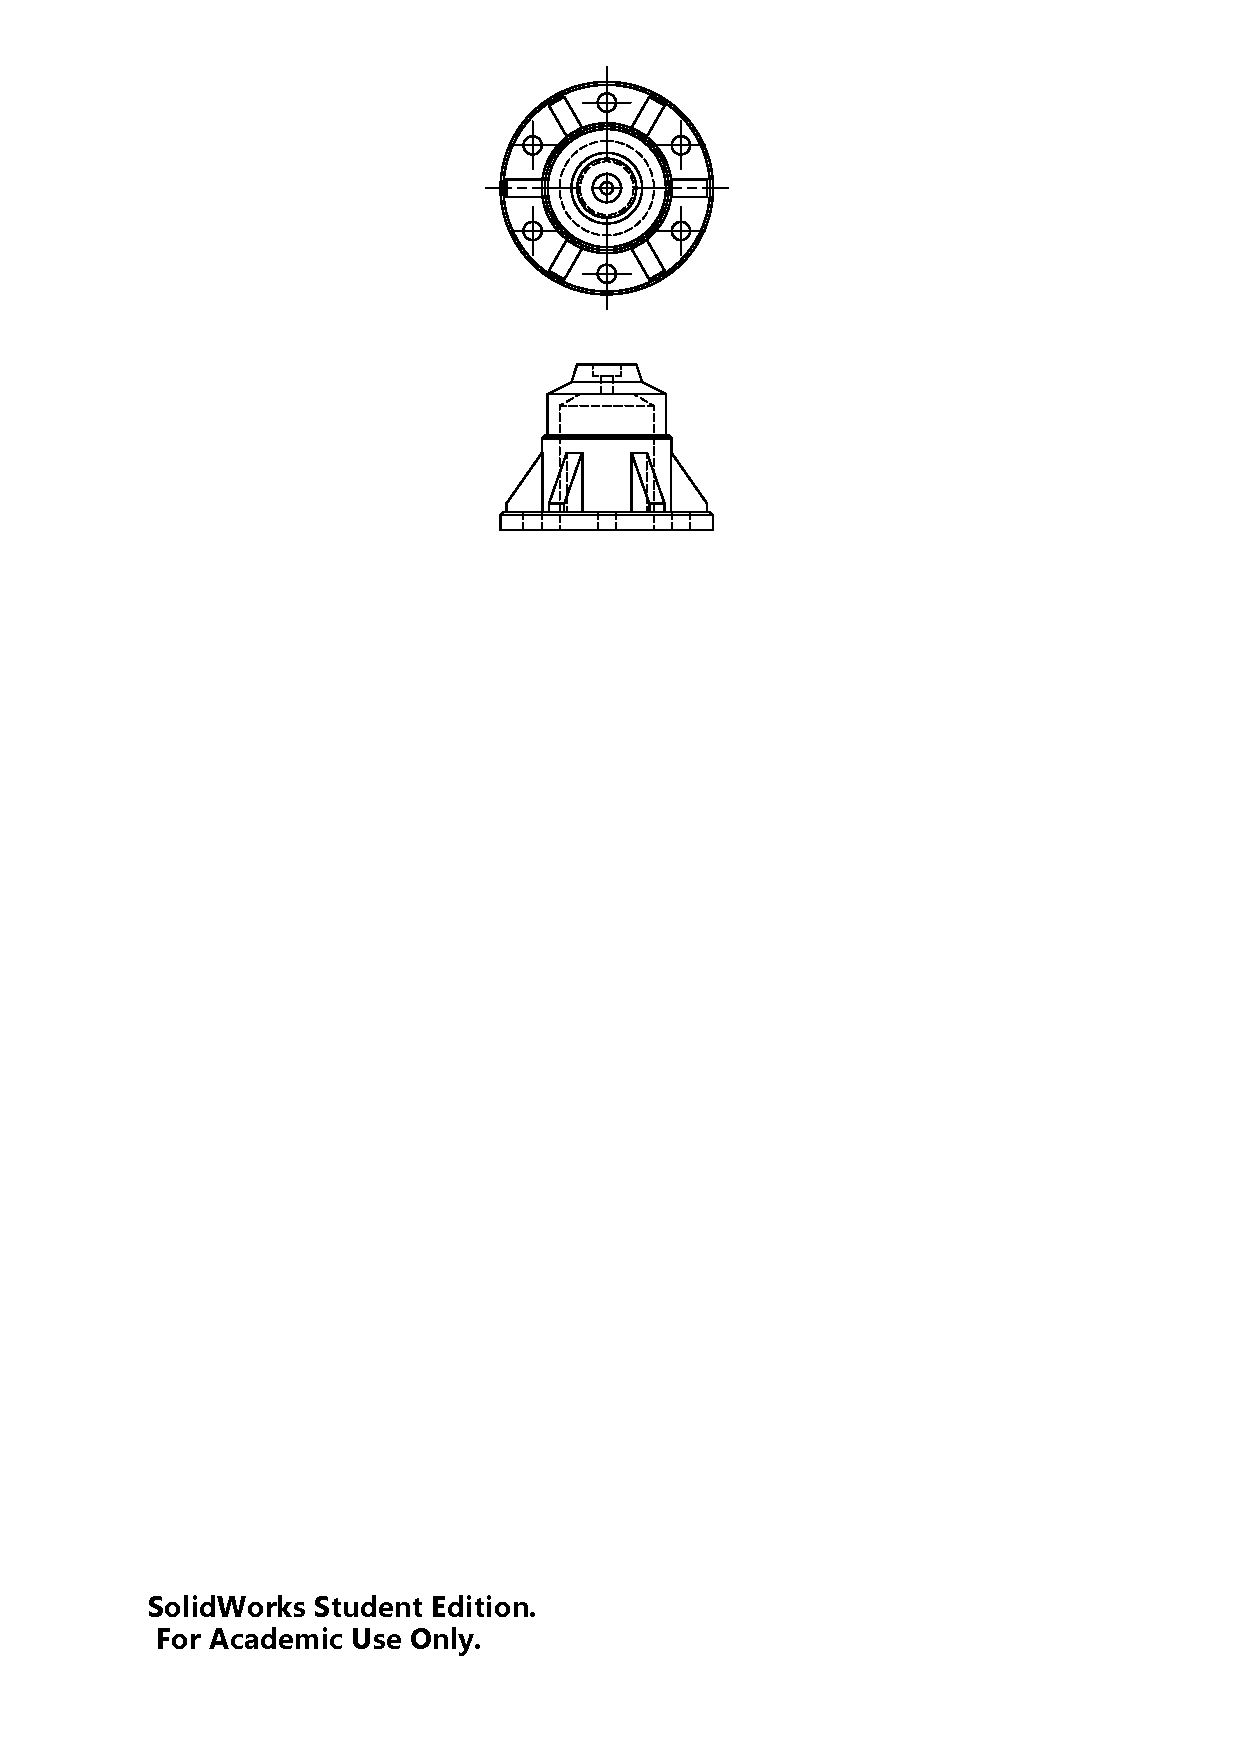
\includegraphics[clip, trim=6cm 19cm 6cm 0cm, width=0.49\linewidth]{figures/mastMount-top}
        }%
        \subfloat[]{
          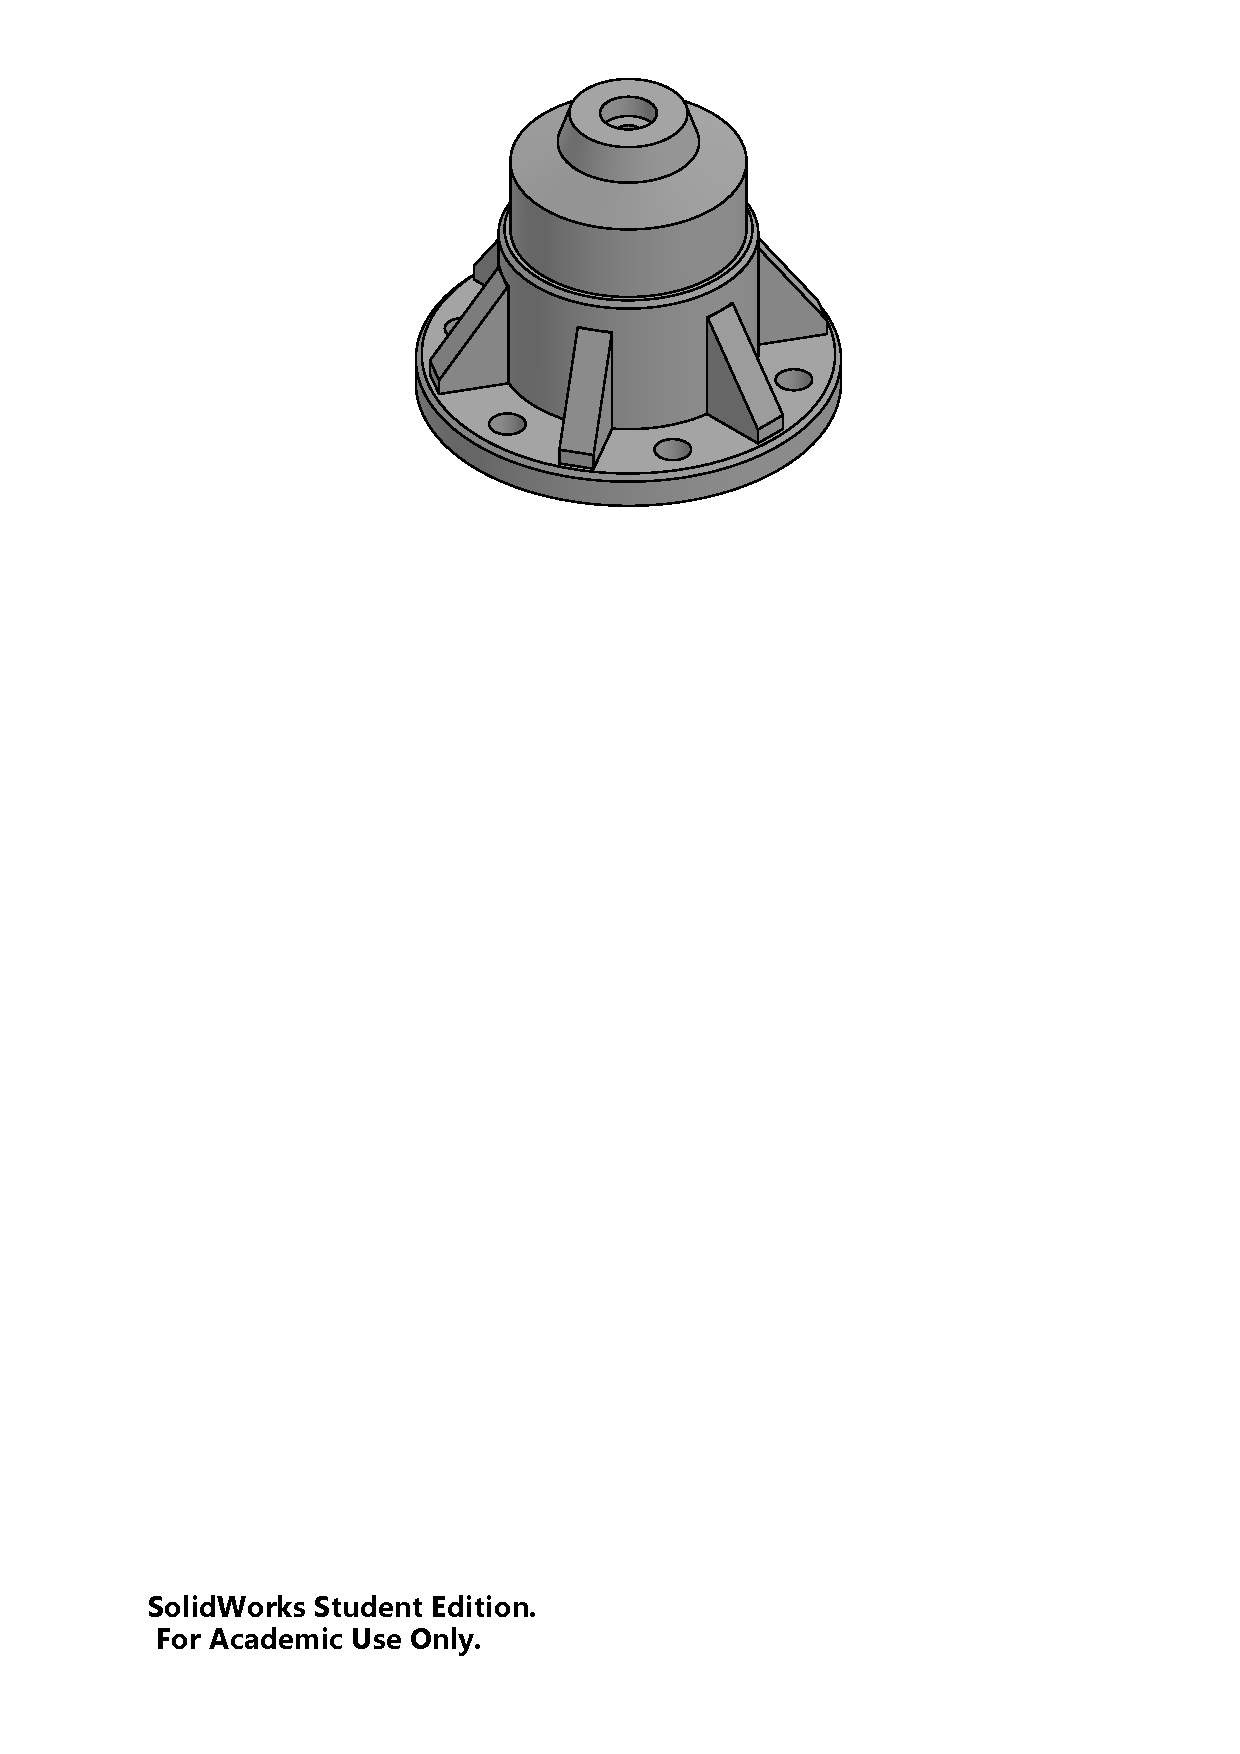
\includegraphics[clip, trim=3cm 17cm 3cm 1cm, width=0.49\linewidth]{figures/mastMount-top-iso}
        }
        \caption[Detailed drawings of the neck mount component in the head and neck sub-assembly]{Detailed drawings of the neck mount component in the head and neck sub-assembly}
        \label{fig:mechDesign-neckMount}
        \end{figure}

      \subheading{Neck Hinge and Actuation}\\\\
        The center piece in the neck-head assembly, referred to as the neck hinge, was designed to facilitate the mounting of two servos: one for pan movement and the other for pitch movement. As discussed, the pan-axis, servo which by definition was facing downwards towards the rover deck surface, would fit into hole in the top of the neck mount and support the rest of the neck-head assembly. Fitted into the neck hinge component was the pitch-axis servo which was displaced from the pan-axis servo by 90 degrees. Multiple configurations involving the placement of the servos were considered and the one which had the smallest volumetric footprint as well as required the least amount of 3D printing material was chosen. This configuration had the servos positioned flat against each other with support material positioned at the servo mounting holes, the assembly of which can be seen in Figure~\ref{fig:mechDesign-neckHingeServoSubExpl}. Figure~\ref{fig:mechDesign-neckHinge} shows the detailed drawing of the neck hinge component without the servos.
        
        \begin{figure}[h!]
        \centering
        \subfloat[]{
          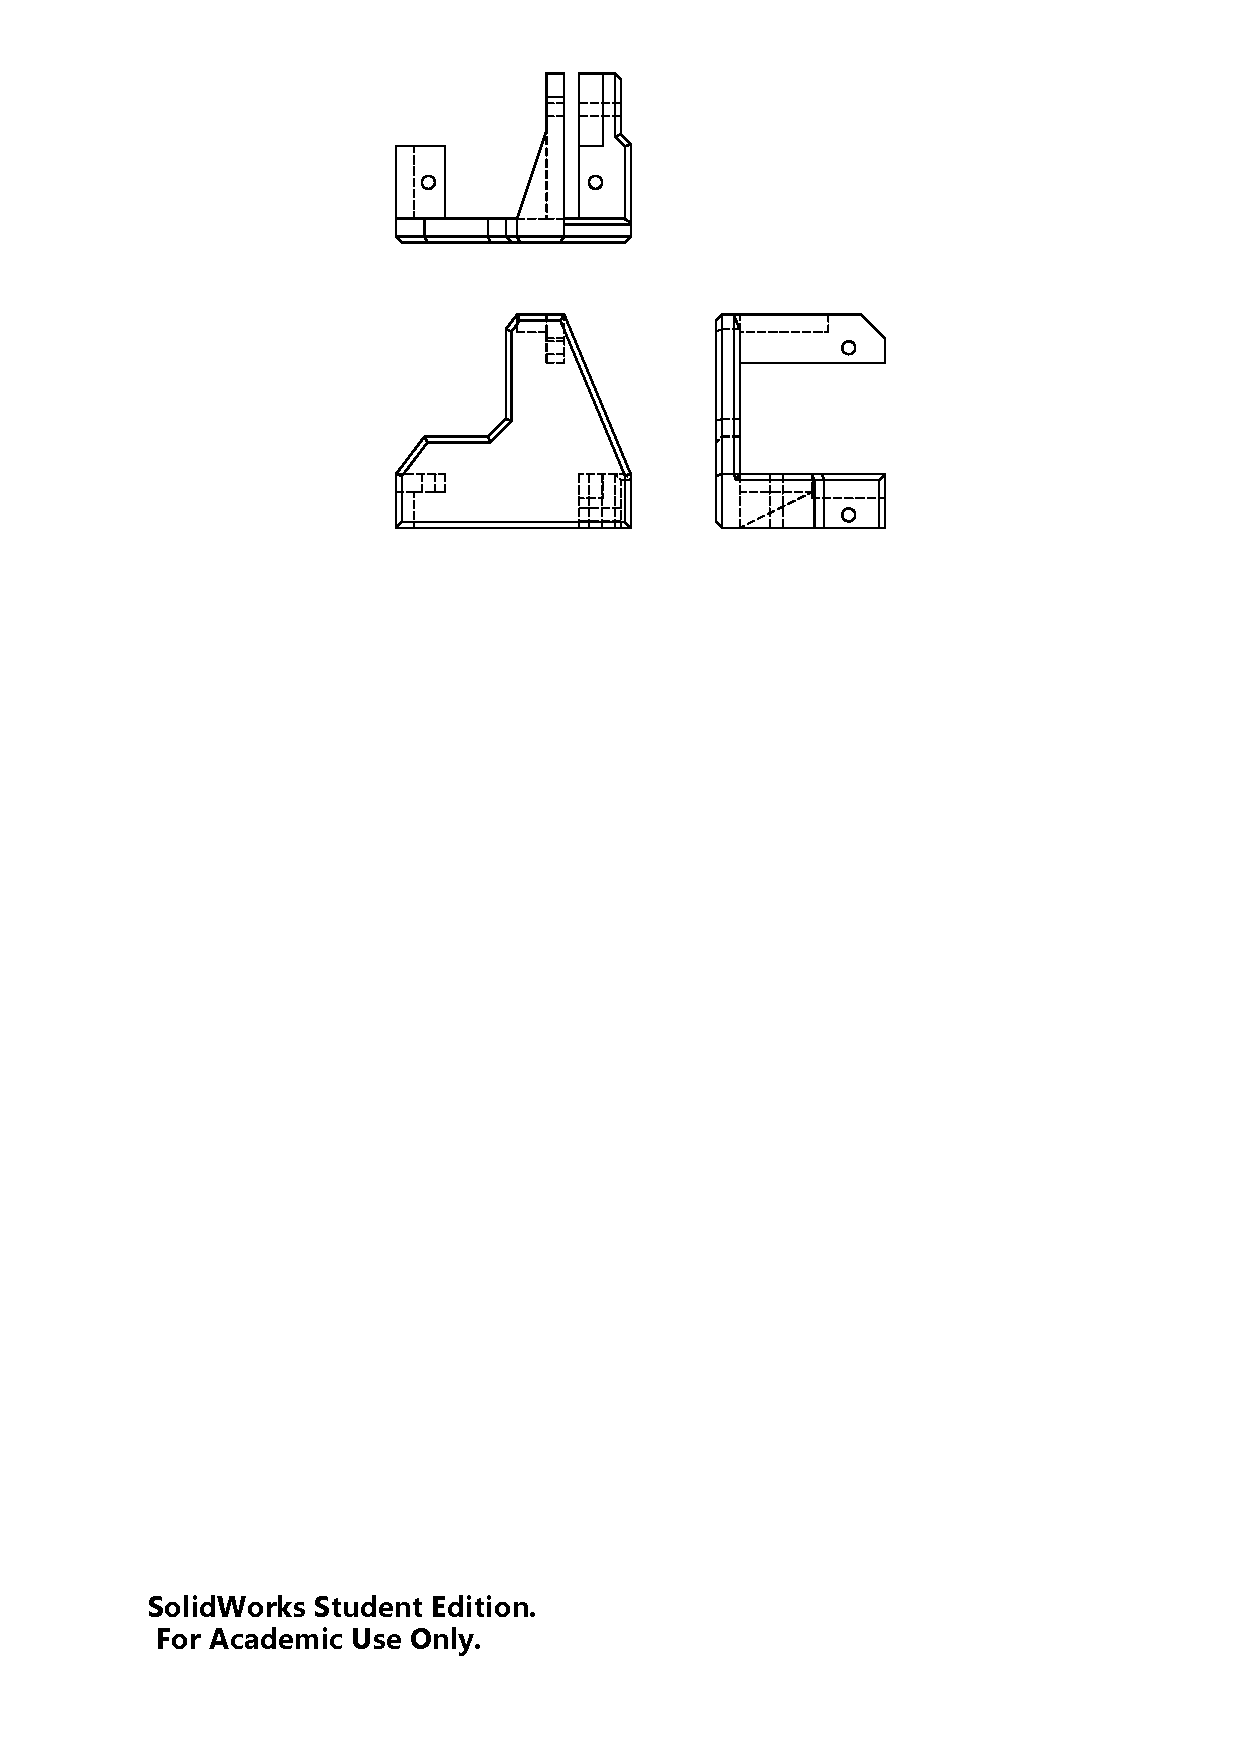
\includegraphics[clip, trim=6cm 19cm 6cm 0cm, width=0.44\linewidth]{figures/neck-hinge}
        }%
        \subfloat[]{
          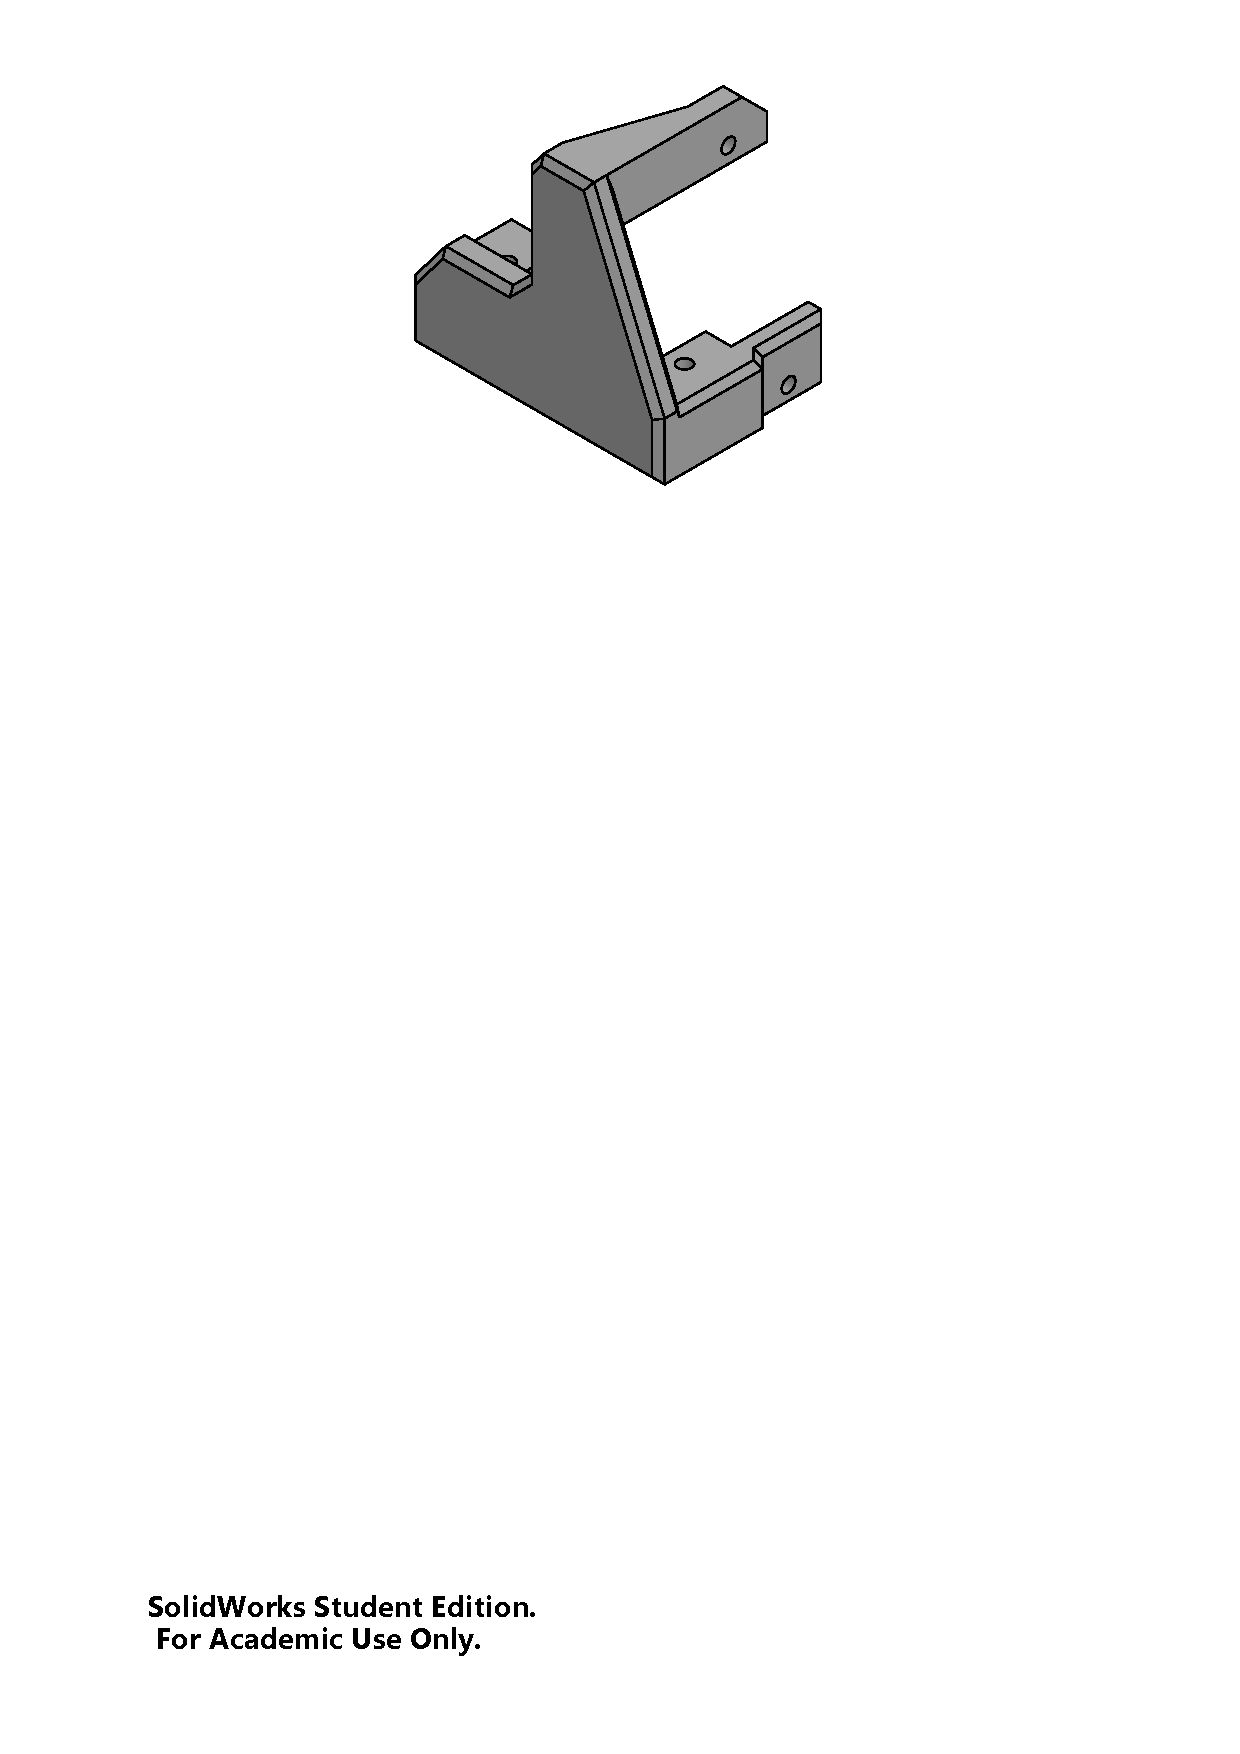
\includegraphics[clip, trim=4cm 18cm 4cm 1cm, width=0.55\linewidth]{figures/neck-hinge-iso}
        }
        \caption[Detailed drawings of the neck hinge component in the head and neck sub-assembly]{Detailed drawings of the neck hinge component in the head and neck sub-assembly}
        \label{fig:mechDesign-neckHinge}
        \end{figure}
        
        \begin{figure}[h!]
          \centering
          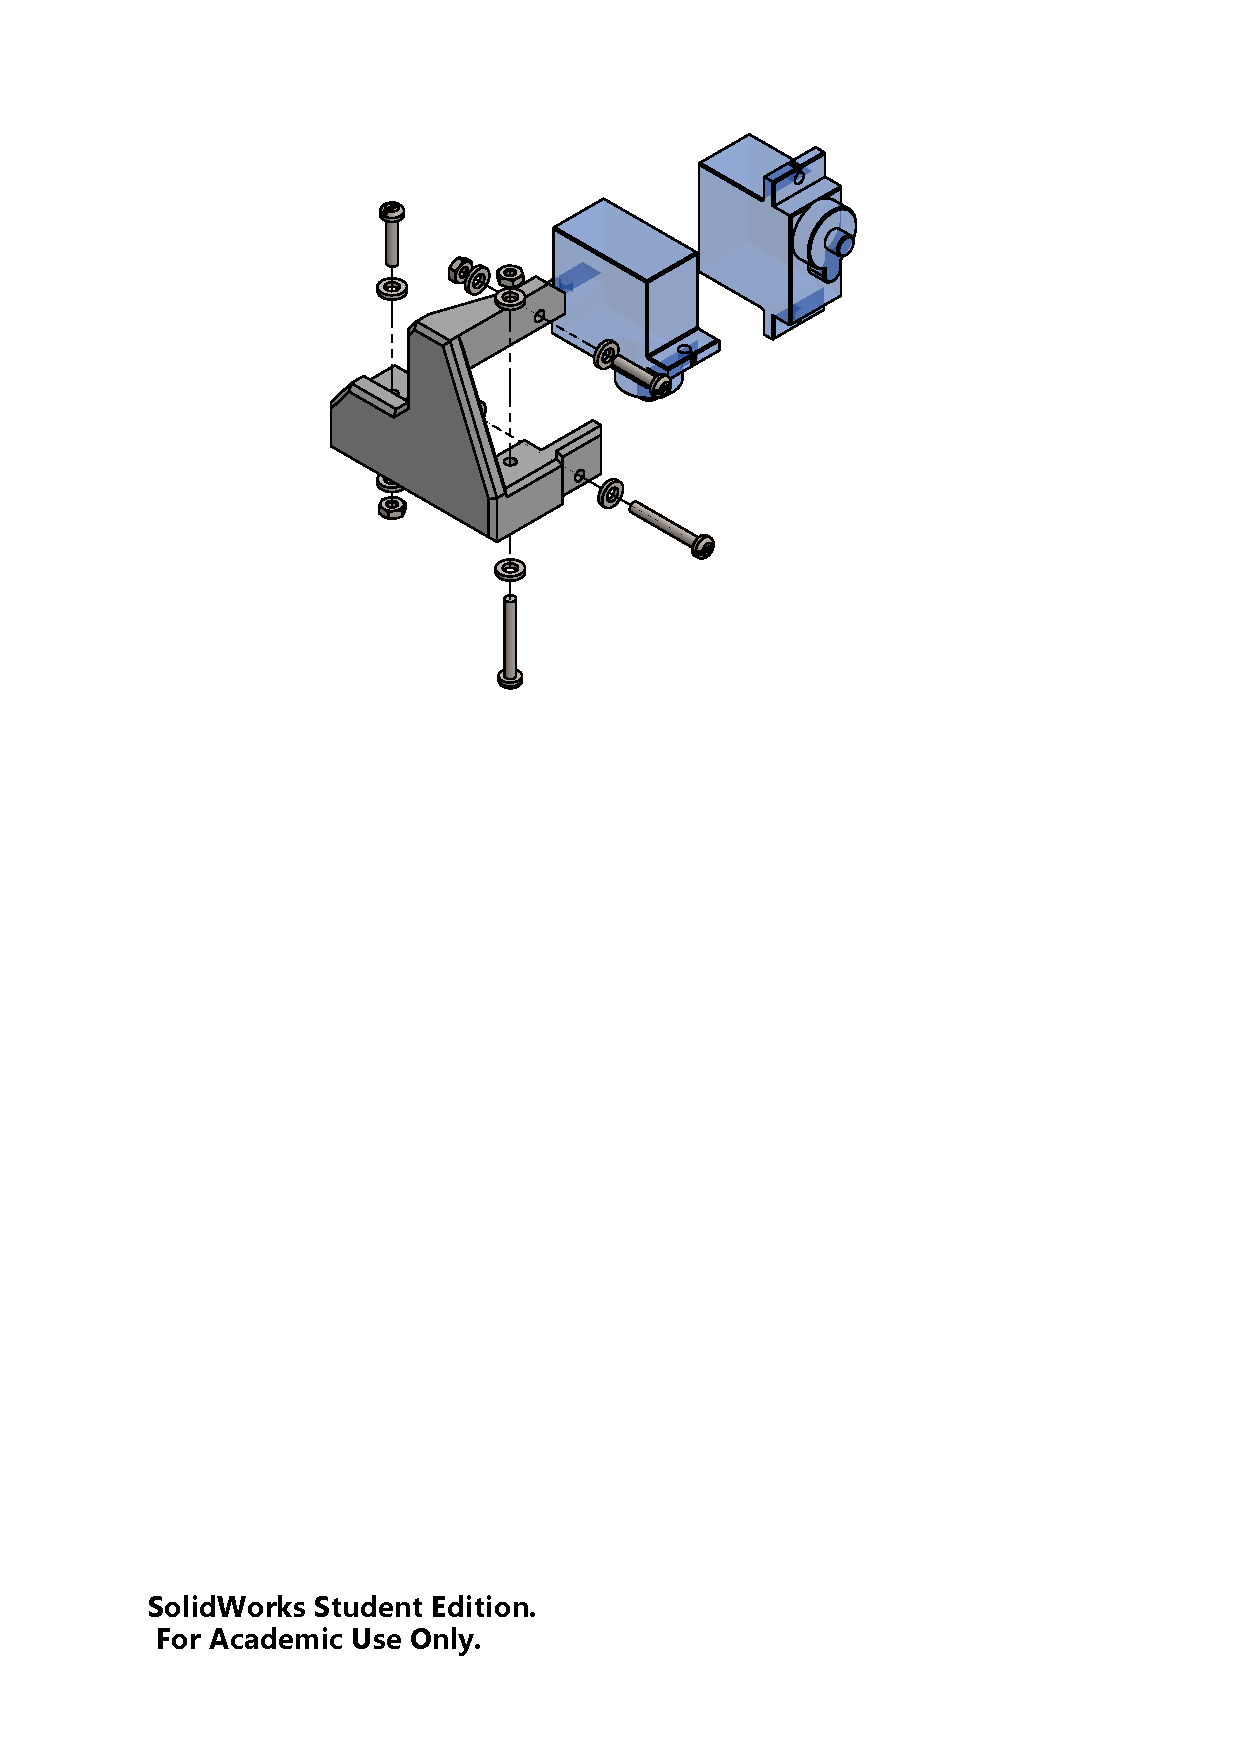
\includegraphics[clip, trim=3cm 17cm 3cm 1cm, width=1\linewidth]{figures/neck-hinge-servo-sub-expl}
          \caption[Exploded isometric view of the neck hinge and servo assembly]{Exploded isometric view of the neck hinge and servo assembly}
          \label{fig:mechDesign-neckHingeServoSubExpl}
        \end{figure}

      \subheading{Head}\\\\
        The head sub-assembly provided an enclosure for the web camera as well as a surface onto which the head ultrasonic sensor was mounted. As mentioned, the very least number of components required for the two-degrees-of-freedom assembly was three, however, the head sub-assembly required two additional pieces. These components were added to reduce the complexity of the components and therefore improve on 3D printing time and material use.
        
        The head enclosure consisted of two components: a flat base and a box-like canopy. The canopy included an arched cut-out which allowed the camera, mounted on the inside, to view the outside world. The canopy was designed as a separate piece so that it could be removed to install and access the camera. As a minimisation of the footprint required by the fastening of the canopy to the base component, inset neodymium magnets were placed at all four corners of the canopy and base components such that the canopy clicked onto the base. Additionally, the canopy was designed to resemble as closely as possible the head on \textit{Curiosity} as this was one of the rover's more recognisable and characteristic components from an aesthetic perspective.
        
        The second extra piece included in the head sub-assembly was a right-angled bracket designed to be mounted to the shaft of the pitch-axis servo using a cross-shaped servo horn and fastened to the bottom of the head base component.
        
        Figures~\ref{fig:mechDesign-headBasePlate}, \ref{fig:mechDesign-headCanopy} and \ref{fig:mechDesign-headRightBracket} show detailed views of the three head components.

        \begin{figure}[h!]
        \centering
        \subfloat[]{
          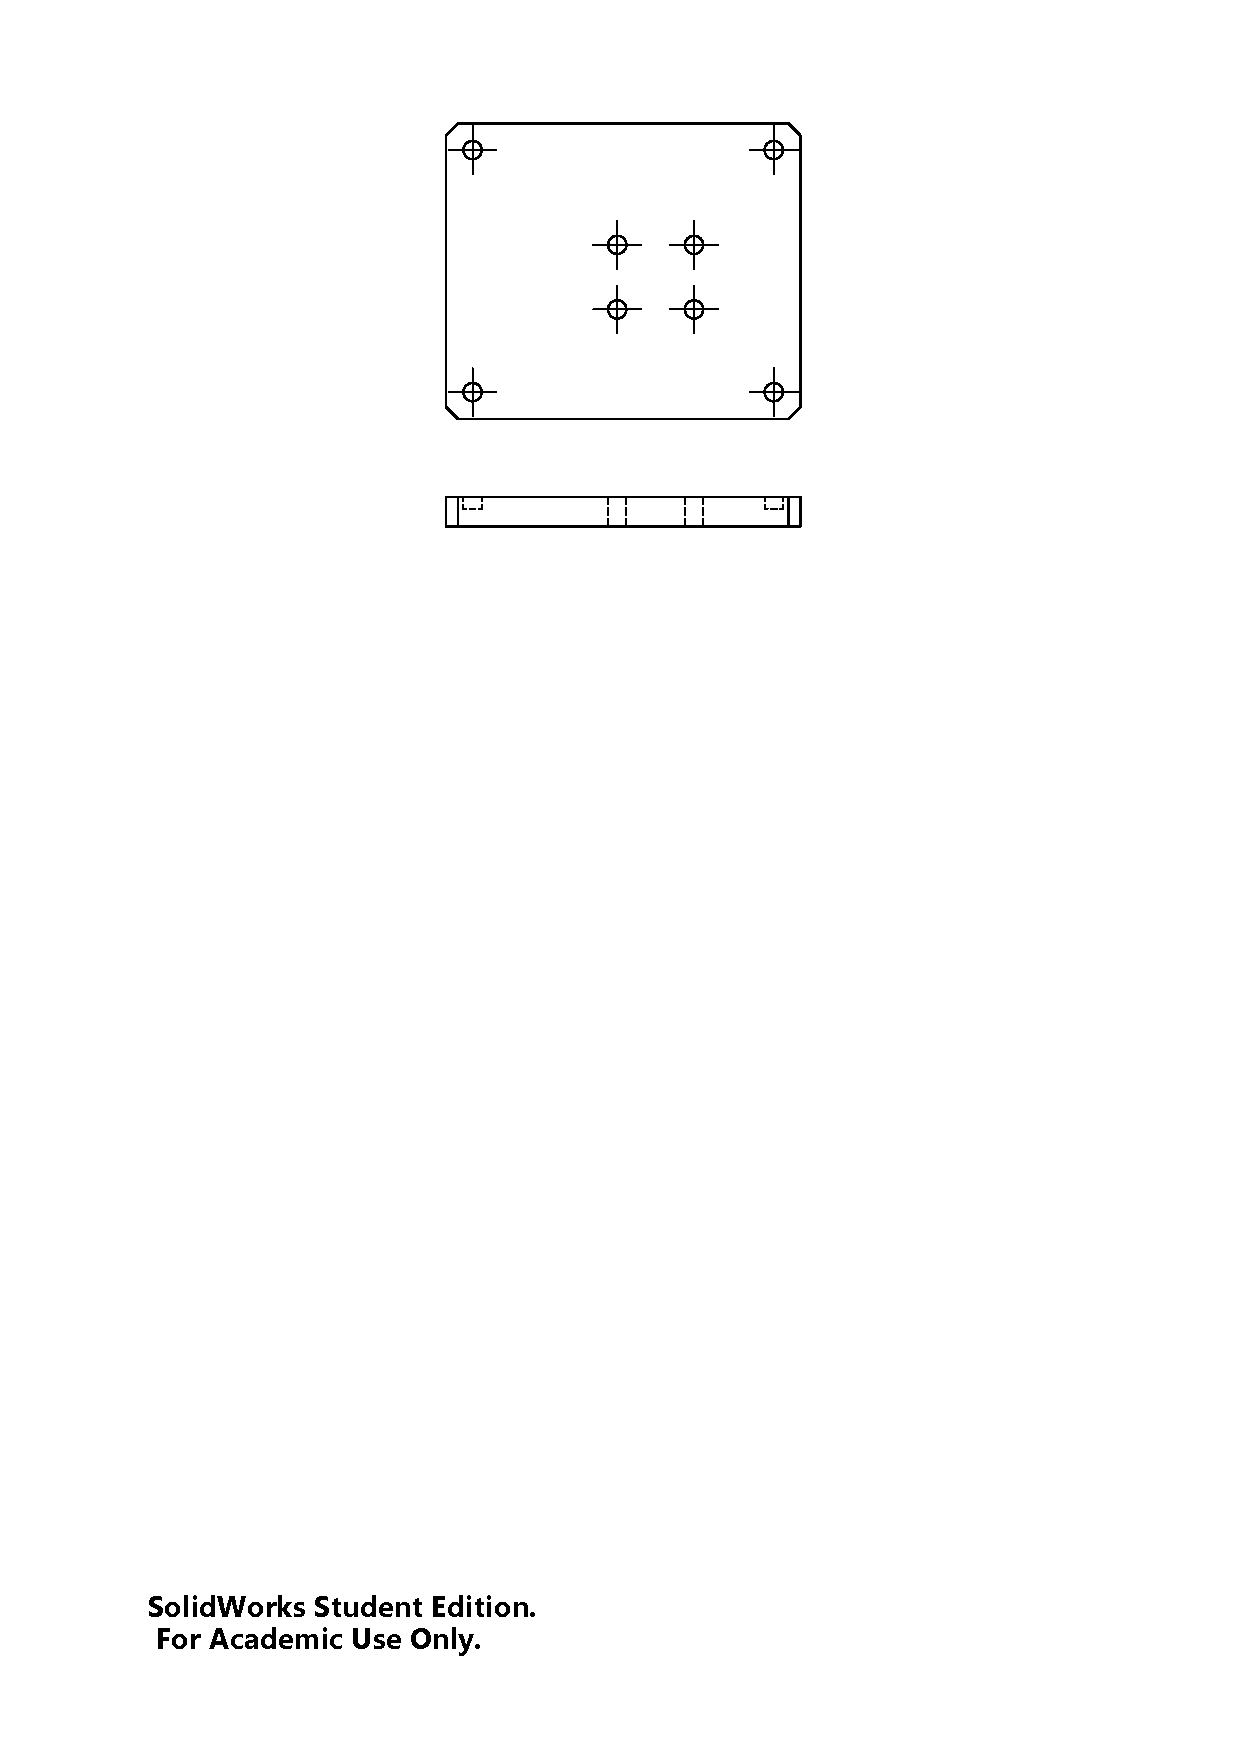
\includegraphics[clip, trim=6cm 19cm 6cm 0cm, width=0.44\linewidth]{figures/headBaseplate}
        }%
        \subfloat[]{
          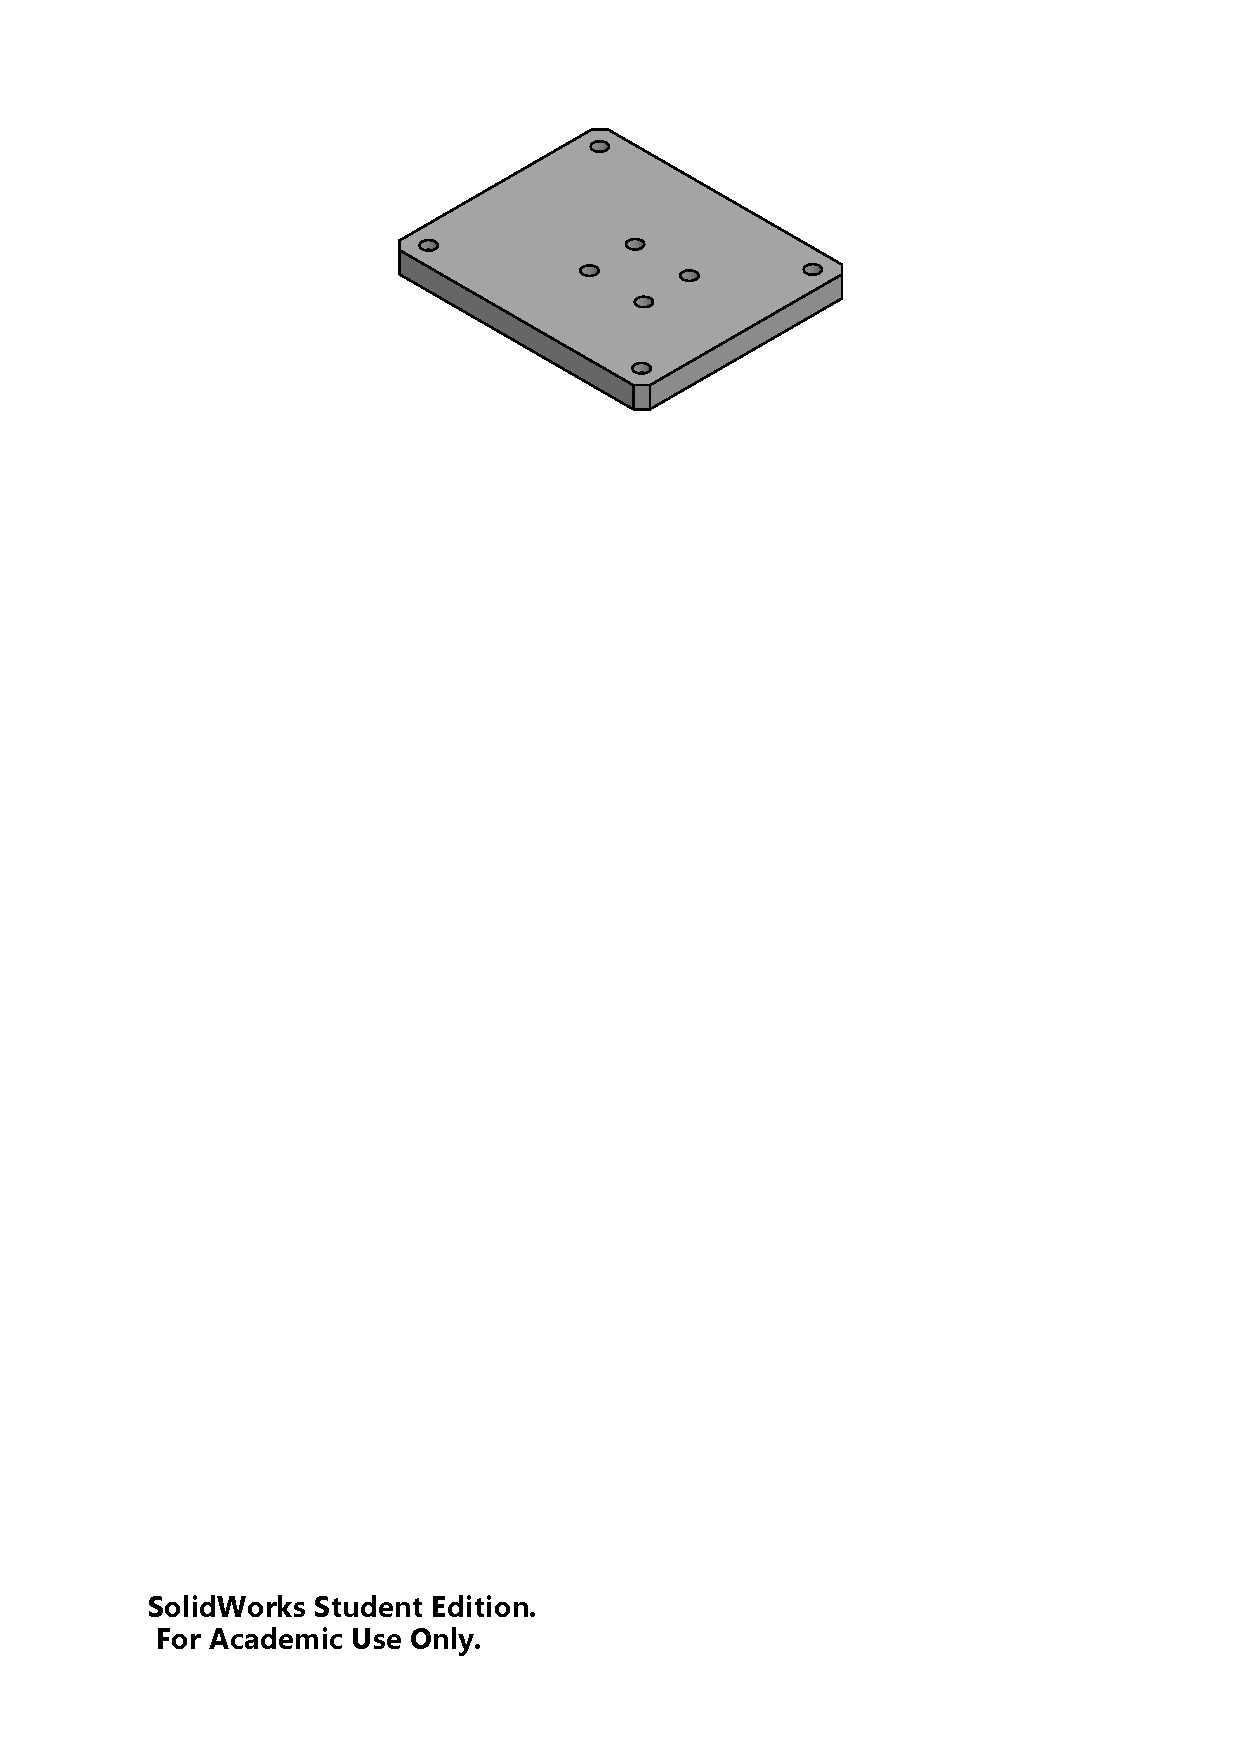
\includegraphics[clip, trim=4cm 18cm 4cm 1cm, width=0.55\linewidth]{figures/headBaseplate-iso}
        }
        \caption[Detailed drawings of the head base component in the head and neck sub-assembly]{Detailed drawings of the head base component in the head and neck sub-assembly}
        \label{fig:mechDesign-headBasePlate}
        \end{figure}

        \begin{figure}[h!]
        \centering
        \subfloat[]{
          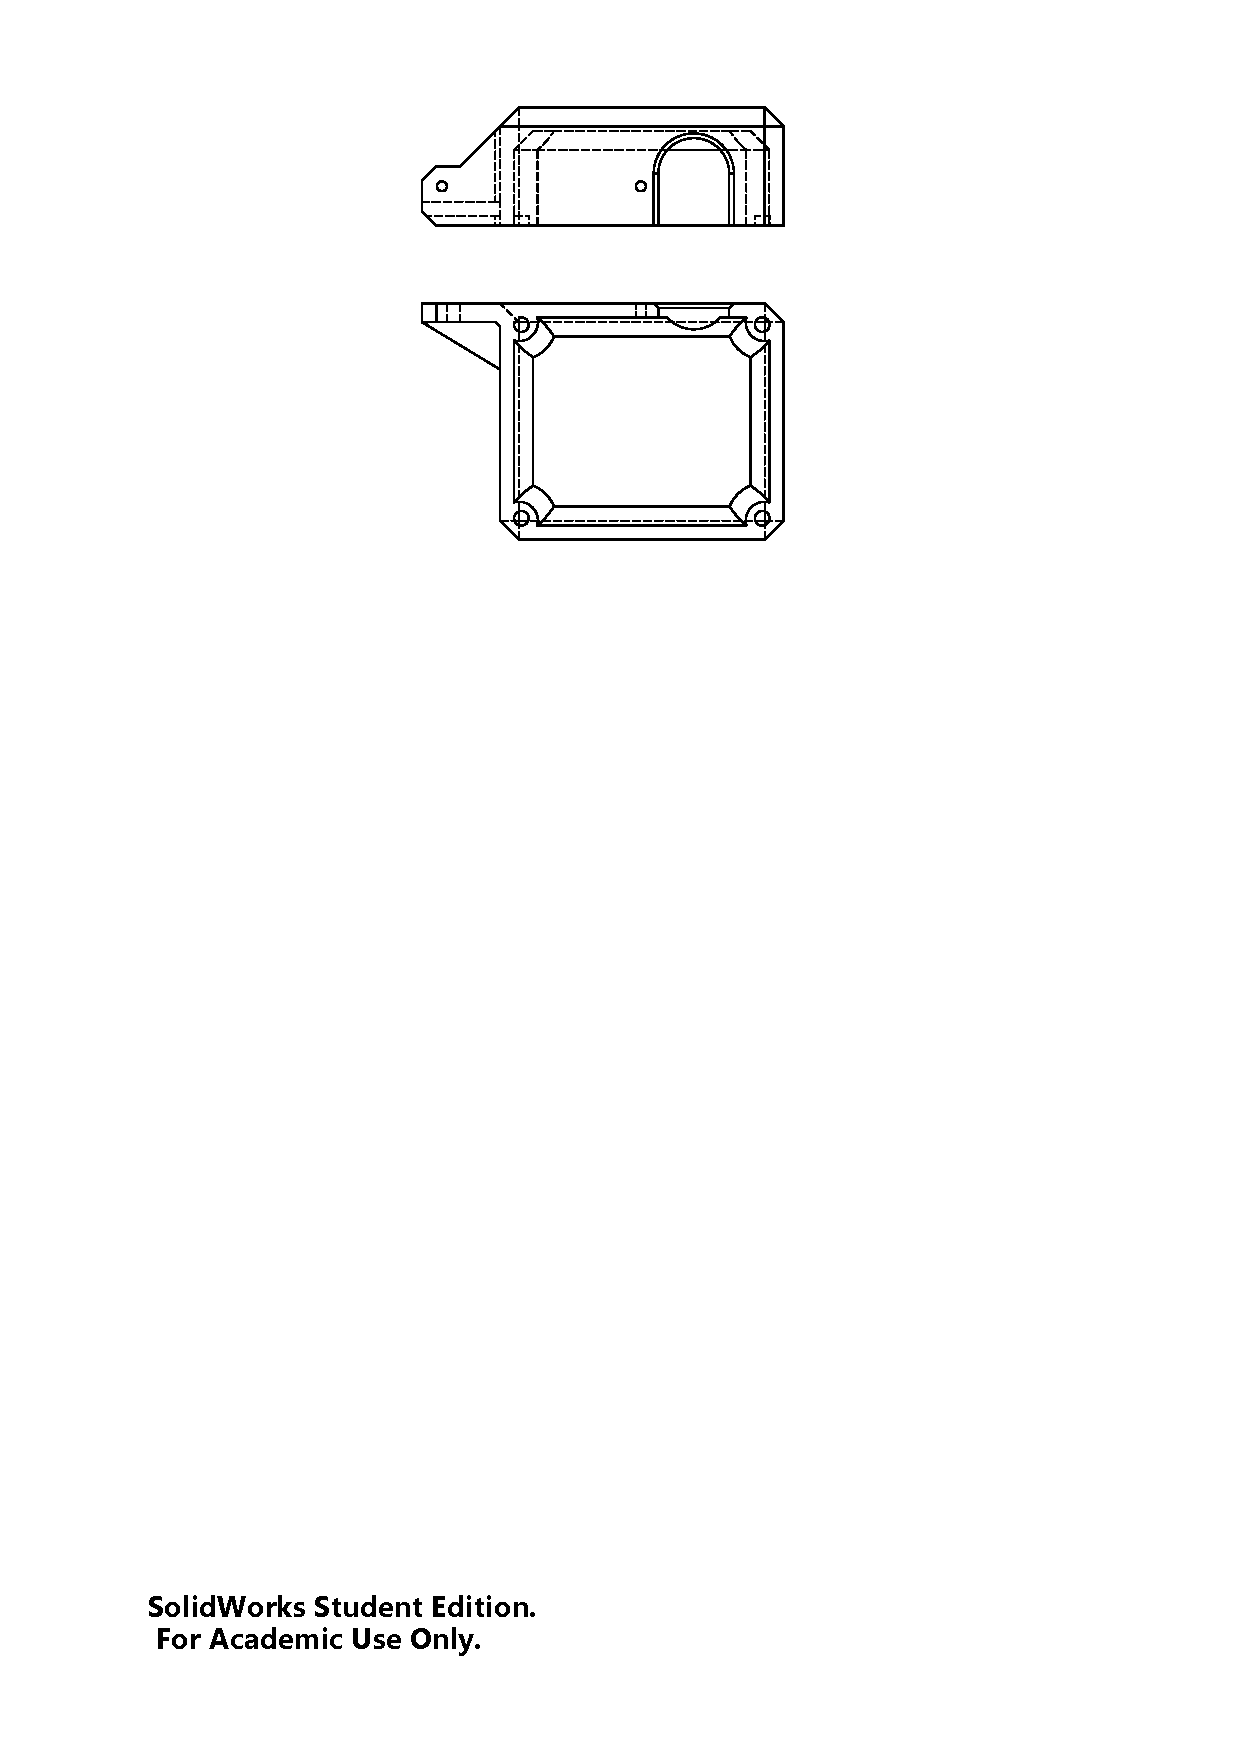
\includegraphics[clip, trim=6cm 19cm 6cm 0cm, width=0.44\linewidth]{figures/head-canopy}
        }%
        \subfloat[]{
          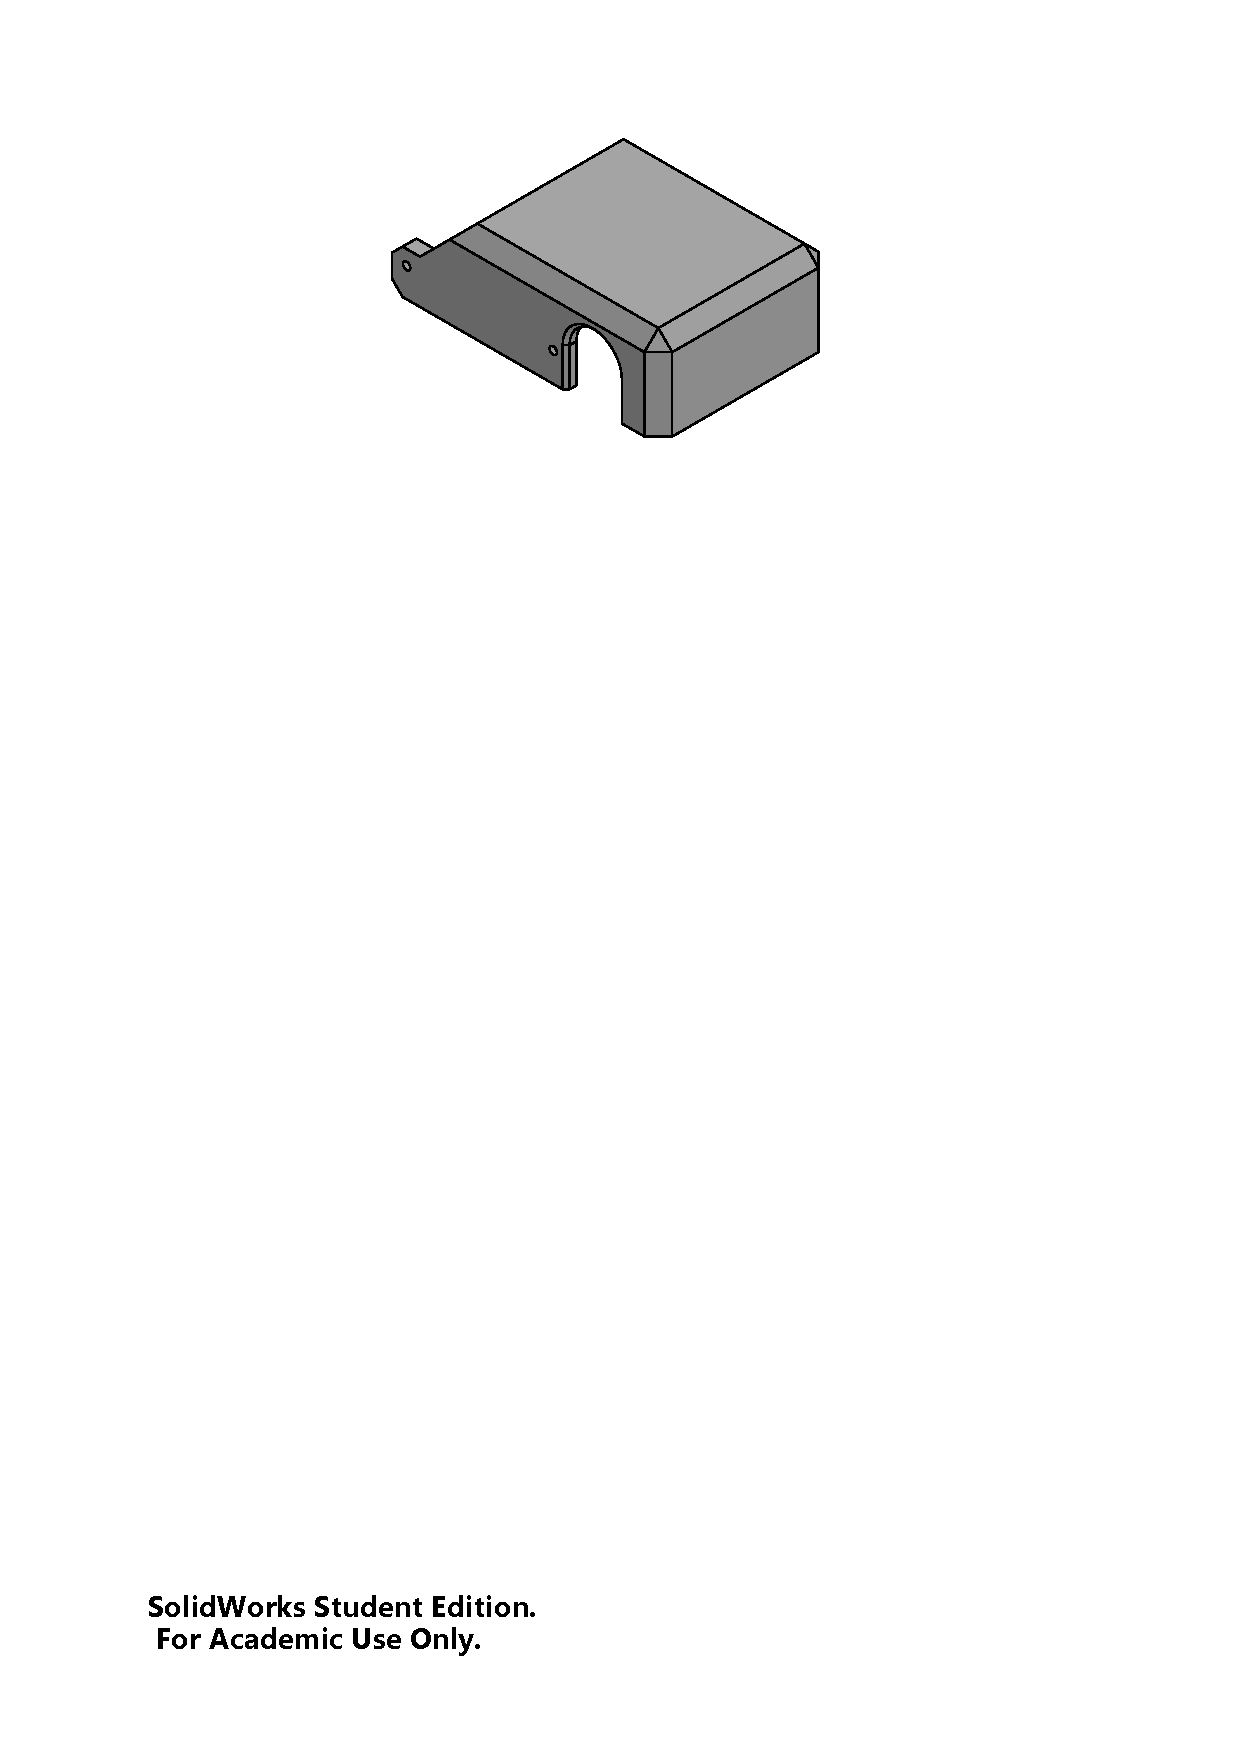
\includegraphics[clip, trim=4cm 18cm 4cm 1cm, width=0.55\linewidth]{figures/head-canopy-iso}
        }
        \caption[Detailed drawings of the head canopy component in the head and neck sub-assembly]{Detailed drawings of the head canopy component in the head and neck sub-assembly}
        \label{fig:mechDesign-headCanopy}
        \end{figure}

        \begin{figure}[h!]
        \centering
        \subfloat[]{
          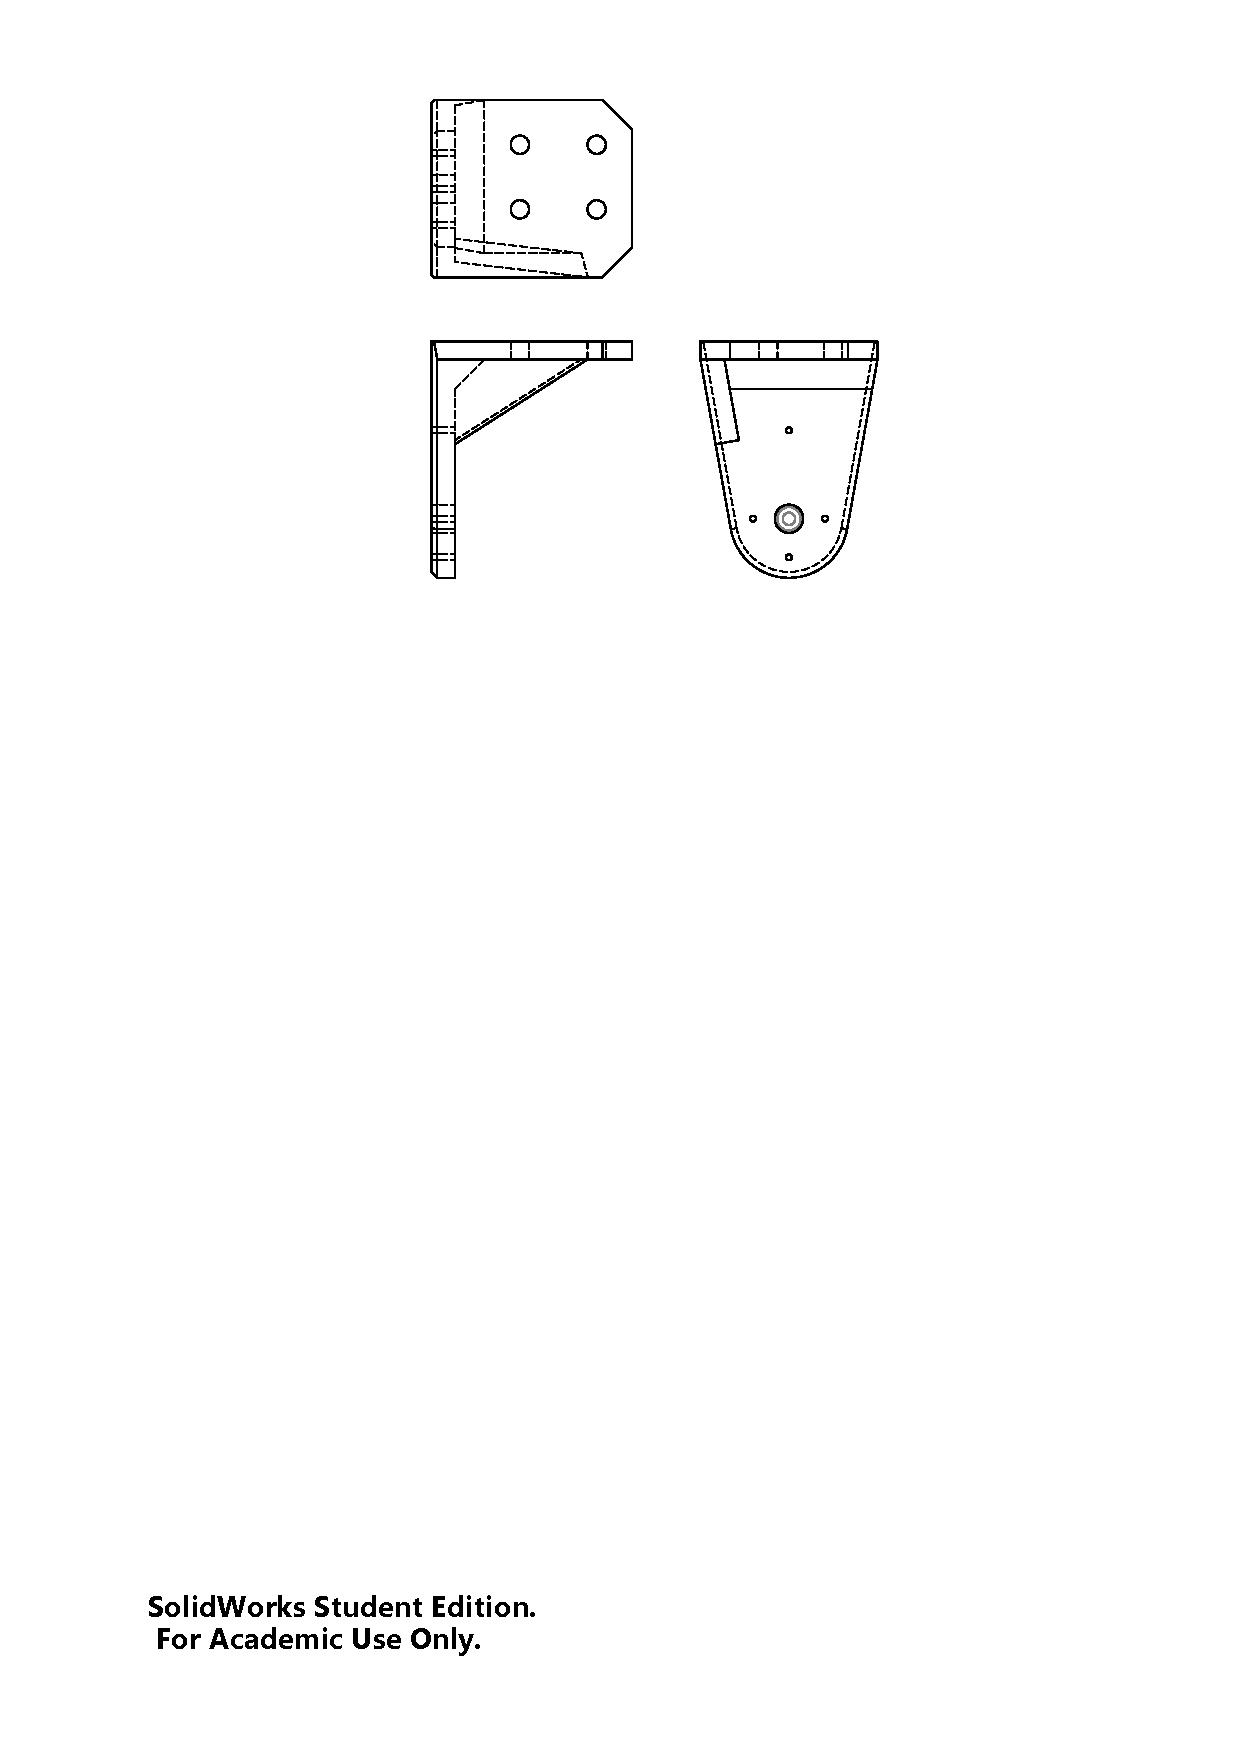
\includegraphics[clip, trim=6cm 19cm 6cm 0cm, width=0.44\linewidth]{figures/right-bracket}
        }%
        \subfloat[]{
          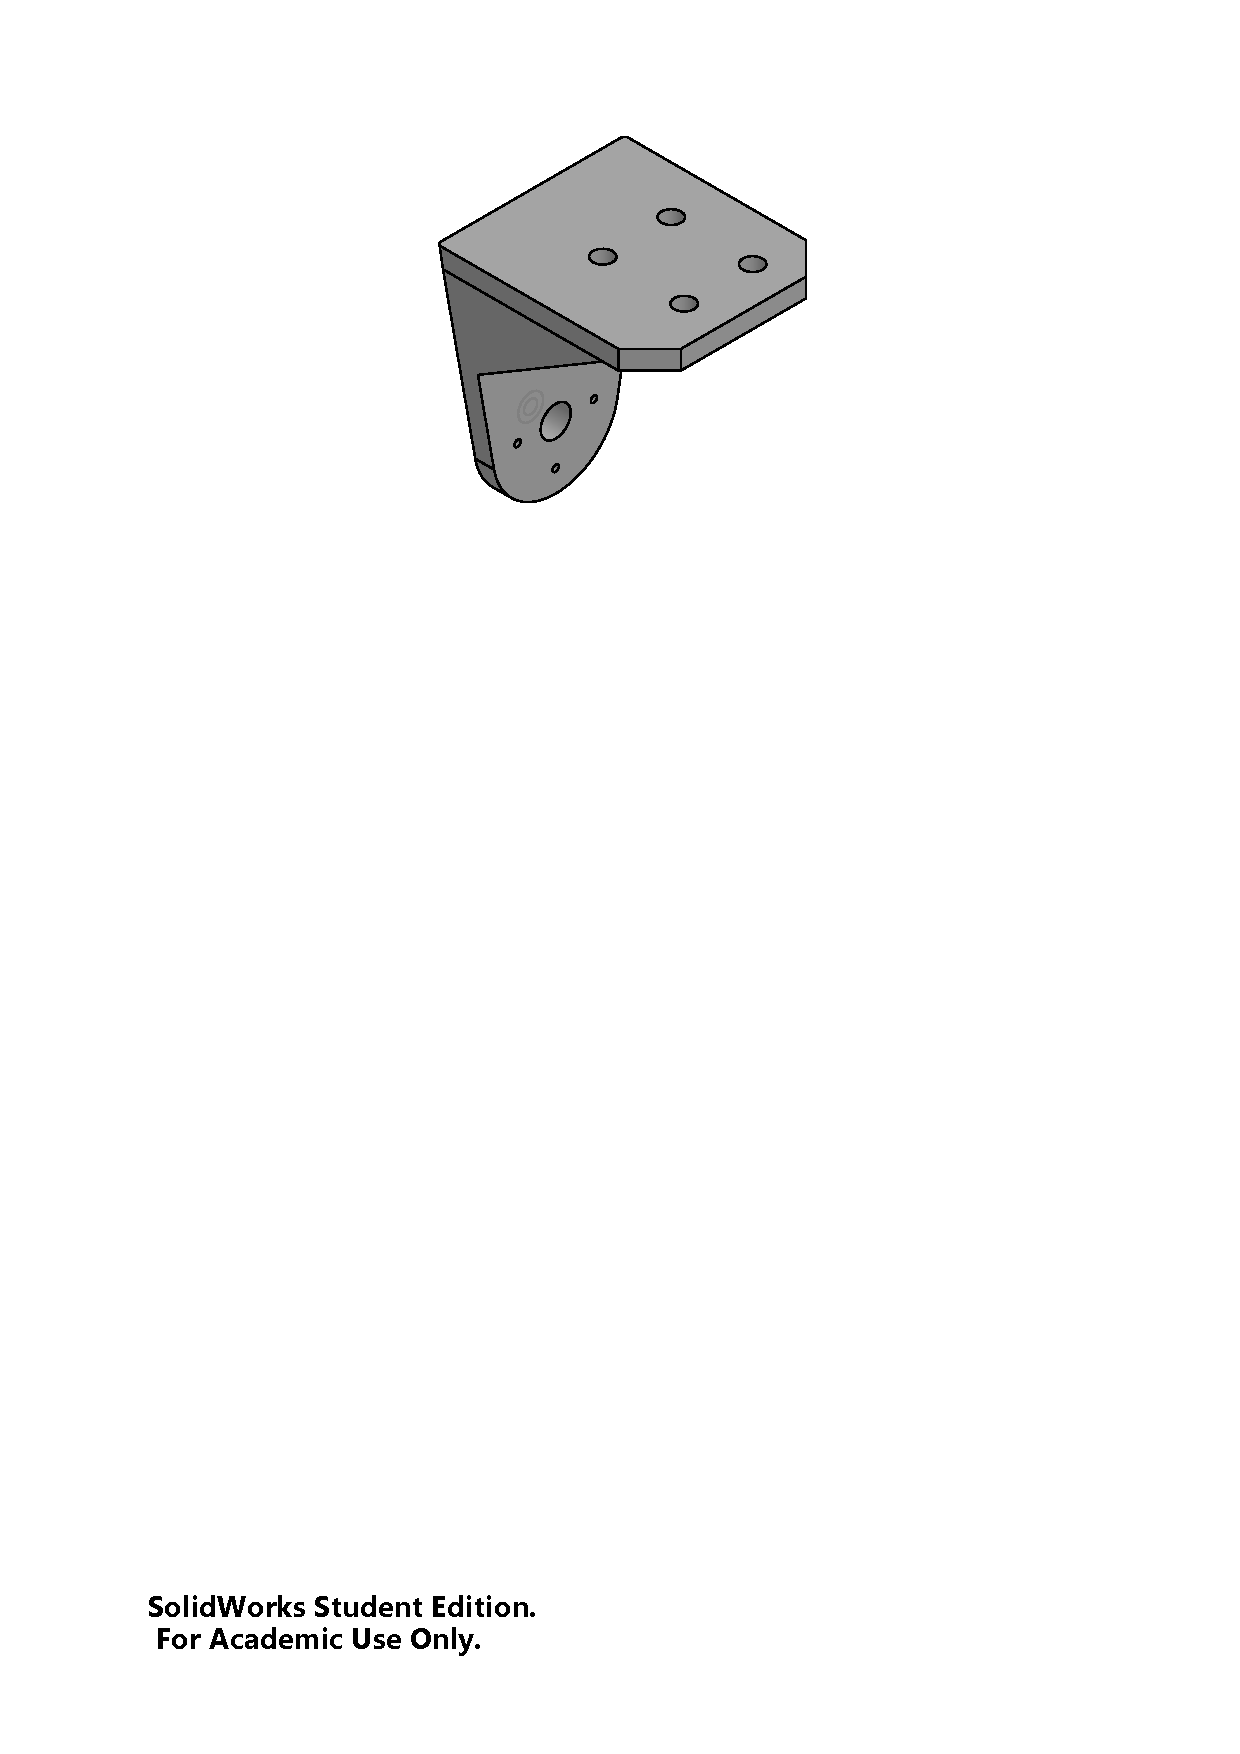
\includegraphics[clip, trim=4cm 18cm 4cm 1cm, width=0.55\linewidth]{figures/right-bracket-iso}
        }
        \caption[Detailed drawings of the right bracket component in the head and neck sub-assembly]{Detailed drawings of the right bracket component in the head and neck sub-assembly}
        \label{fig:mechDesign-headRightBracket}
        \end{figure}

      \subheading{Final Sub-assembly}\\\\
        The final sub-assembly of the neck and head components, including the servos is shown in Figure~\ref{fig:mechDesign-headSubDetail}.
        
        \begin{figure}[h!]
        \centering
        \subfloat[]{
          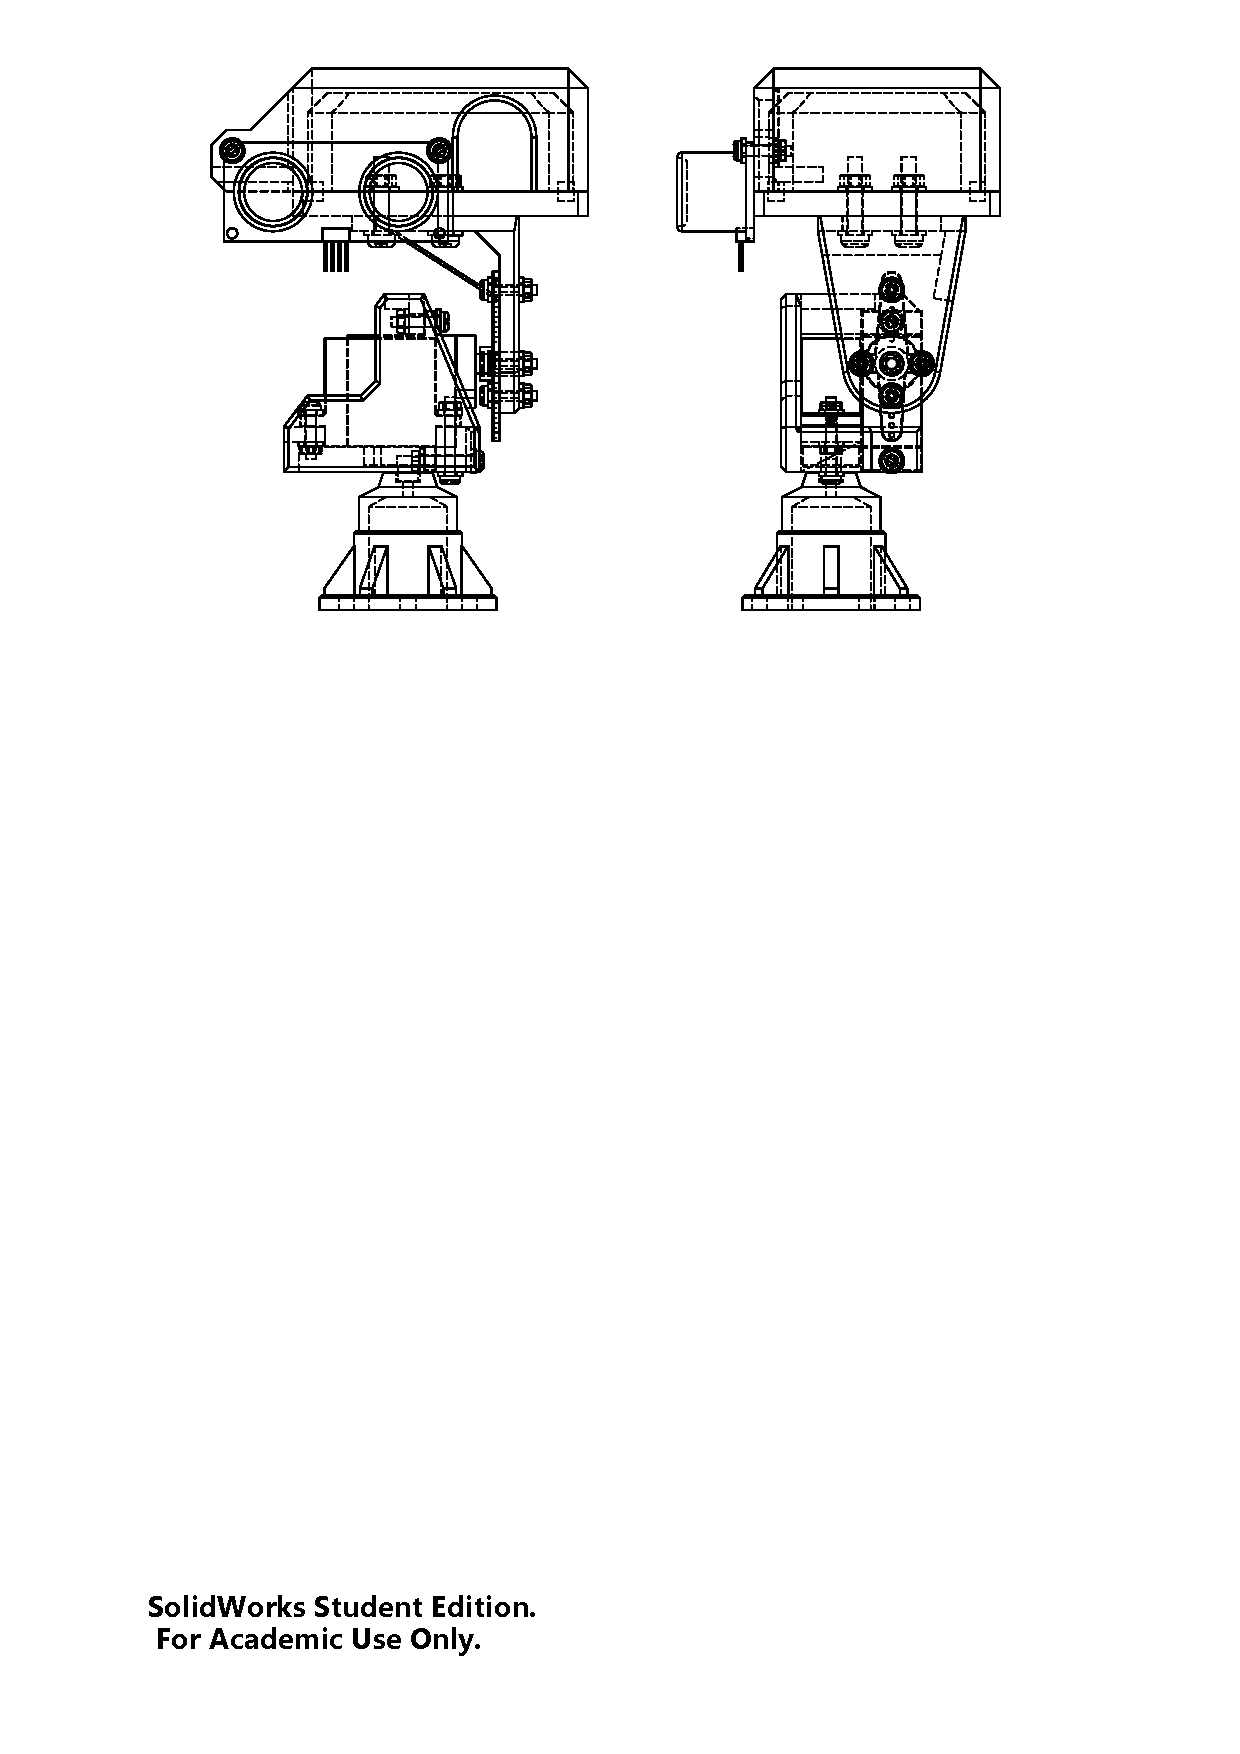
\includegraphics[clip, trim=3cm 18cm 3cm 1cm, width=0.7\linewidth]{figures/headSub}
        }
        \qquad
        \subfloat[]{
          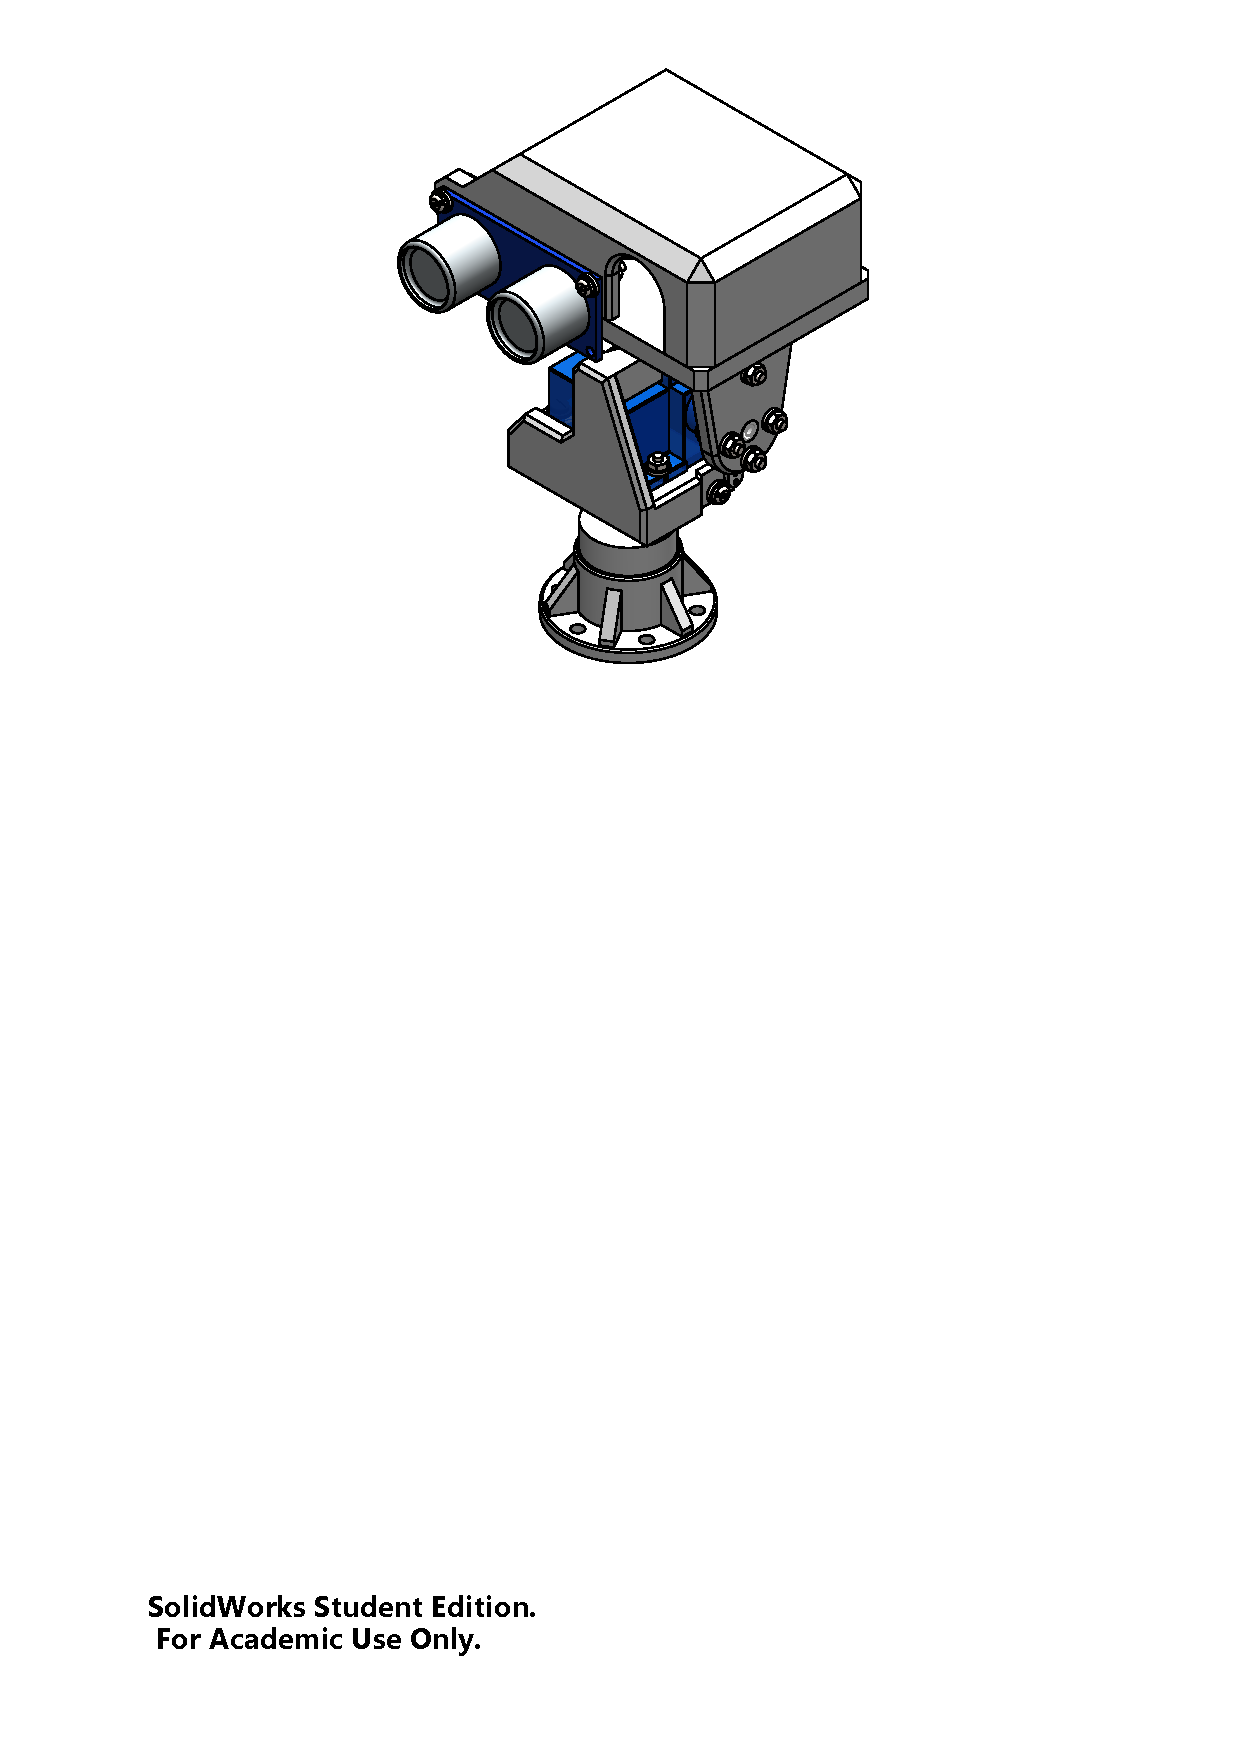
\includegraphics[clip, trim=4cm 17cm 4cm 1cm, width=0.7\linewidth]{figures/headSub-iso}
        }
        \caption[Detailed drawings of the working, dynamic assembly of the head and neck system]{Detailed drawings of the working, dynamic assembly of the head and neck system}
        \label{fig:mechDesign-headSubDetail}
        \end{figure}
        
    \subsubsection{Body}
      The body was a significant part of the rover, designed as a mounting platform for most of the rover's other mechanical and electronic components. The conceptual analysis of the proposed ideas for the assembly of the body settled on the use of acrylic sheet. The body was rectangularly box-shaped and, for the purpose of access to the electronics which were to be mounted internally, the bottom was left open. This meant that five separate panels were designed to be cut from the acrylic sheet and later glued together to form the structure. Once finalising the dimensions of the panels, the required mount points were collated and added to the design. Mounting requirements for the body were as follows:
      
      \begin{itemize}
        \item \textbf{Deck/Top Panel:}
        \begin{itemize}
          \item Neck and head assembly
          \item Differential bar midpoint shaft
          \item Aesthetic detail components
        \end{itemize}
        \item \textbf{Left and Right Panel:}
        \begin{itemize}
          \item Suspension rocker hinge shaft
          \item Bottom cover magnet mount pieces
          \item Aesthetic detail components
        \end{itemize}
        \item \textbf{Rear Panel:}
        \begin{itemize}
          \item Rear ultrasonic sensor
          \item Aesthetic detail components
        \end{itemize}
        \item \textbf{Front Panel:}
        \begin{itemize}
          \item Front ultrasonic sensor
          \item Aesthetic detail components
        \end{itemize}
      \end{itemize}
      
      Aesthetic detail components were those designed to add realism to the rover body and are discussed further in Section~\ref{subsubsec:softDesign-aestheticDetails}. A series of slots were added to the edges of each of the panels which fit into the those of adjacent panels for structural integrity and positioning accuracy whilst glueing. Figure~\ref{fig:mechDesign-perspex} shows the detailed drawings of each of the panels; the same drawings were used for laser cutting the 3mm acrylic sheet.
      
      \begin{figure}[h!]
        \centering
        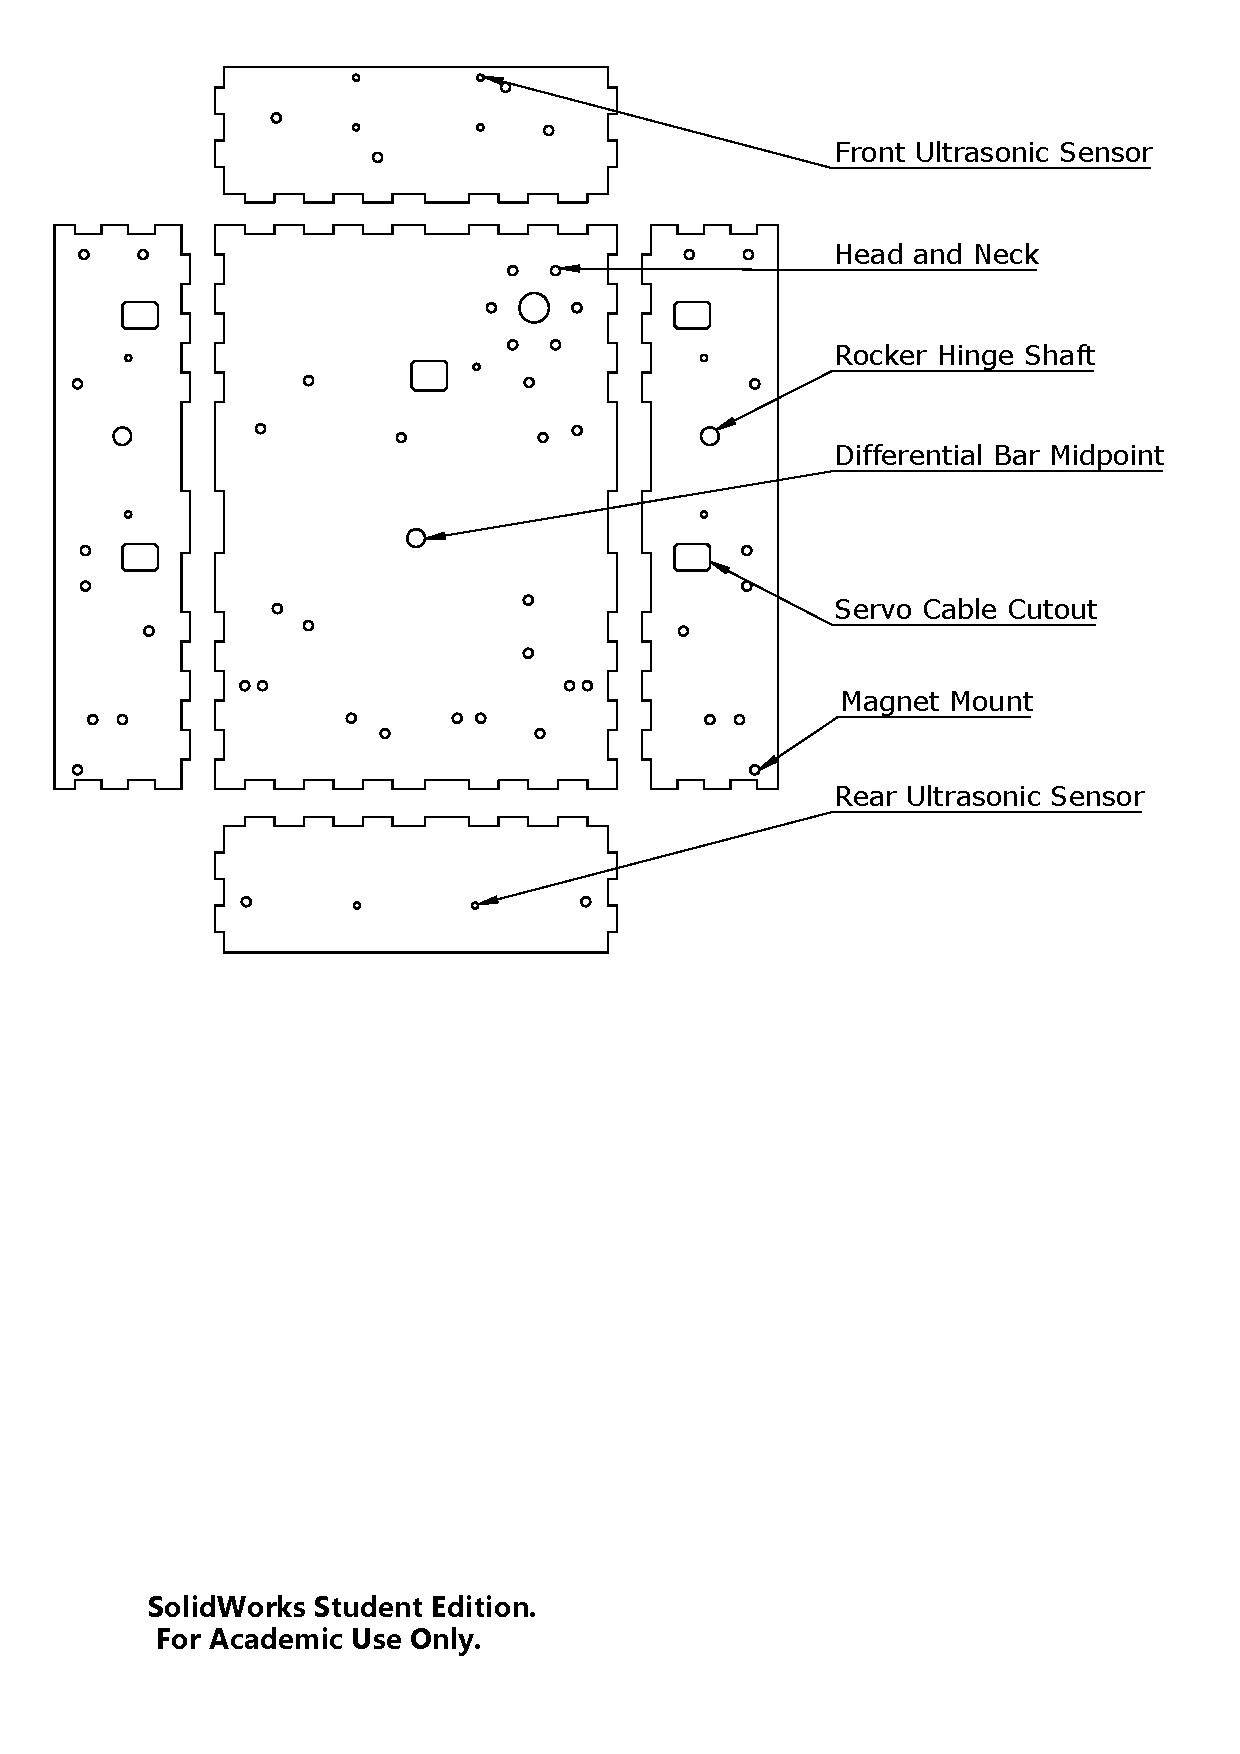
\includegraphics[clip, trim=0cm 13cm 1cm 0cm, width=1\linewidth]{figures/perspex}
        \caption[Drawings of the five acrylic sheet panels including labels indicating the mount points]{Drawings of the five acrylic sheet panels including labels indicating the mount points}
        \label{fig:mechDesign-perspex}
      \end{figure}
      
    \subsubsection{Aesthetic Details}
    \label{subsubsec:softDesign-aestheticDetails}
      To achieve the realism desired for the rover model, a number of extra components were designed to be 3D printed and mounted to the rover body. The design and construction of the body made this suitable and a satisfactory level of realism was possible due to the 3D printing manufacture of the components. The following aesthetic detail components were designed, the drawings of which are included in the set of additional files submitted with this report:
      
      \begin{itemize}
        \item MMRTG
        \item Rear shoulders
        \item Fore shoulders
        \item Four rover deck components
        \item Observation tray
        \item Panel detail pieces for the front, left and right panels
      \end{itemize}
    
  \subsection{Electrical Design}
    The electrical system of the rover involved supplying power to the RCE board, actuation, sensors and camera and included the electrical interfaces between these components. This section covers the design of these interfaces, the supply of power and the detailed choice of electrical hardware and components for this part of the project. Due to project time constraints, use of COTS components wherever possible was made the driving principle off which the electrical design was based. This was also beneficial for individuals wanting to get involved as part of the open sourcing of the project. Including as many COTS components that are available to as many people as possible improved the accessibility of the project and its ease of duplication to benefit education and outreach as a whole.
  
    \subsubsection{Actuation}
      The device for position- and velocity-based actuation during the conceptual design phase was servos of the sub-micro size and after investigation into the availability of multiple models of the servo type, the Hextronics HXT900 servo was chosen. This servo, a 9g, plastic-geared component requiring a 3V-6V supply, offered 180 degrees of movement at a maximum of $0.157$Nm of torque. The range of motion meant that is was suitable for the steering of the four corner wheels as well as pan and pitch actuation of the camera and proximity sensor above the neck sub-assembly. However, the decision to use the servos for driving the four corner wheels meant that the servos required continuous rotation and not a limited range. The continuous motion was also required to be controlled from the perspective of velocity and not position. It was found that servos designed for continuous rotation were available but were not within the project budget. An alternative solution was found, whereby the range-limited HXT900s could be altered to result in velocity-controlled continuous servos. These were used and the alterations involved are discussed in Section~\ref{sec:vehicleBuildAndManufacture}.
      
      Standard communication applied for the HXT900 servo component, an analog-type device. The servo required power and ground connections and a third line for a PWM signal. The pulse width determined, in the case of the range-limited servos, position, and velocity in the case of the modified continuous servos. This signal was to originate from the Intel Edison board, however, the low-level implementation of PWM signal generation on the device had significant limitations which meant that an alternative means had to be found. Additionally, the Intel Edison Arduino breakout board only offered six PWM signal pins and the rover actuation system required ten. The solution was to use a 16-channel PWM extension board which was compatible with the header and pin layout of the Intel Edison board, allowing for flexible control of many servo components. The PWM extension, manufactured by Adafruit, interfaced with the Intel Edison by means of a two-wire I$^2$C connection which meant that the rest of the Intel Edison board's pins were available for use elsewhere. The PWM extension also included short-circuit and reverse-polarity protection for increased system robustness as well as a breadboard section which was used for multiple other electrical subsystems discussed further.
      
    \subsubsection{Sensors}
      The three HC-SR04 ultrasonic proximity sensors provided elementary spatial awareness to the rover, specifically to the control system as part of the RCE. The sensors, mounted to the front and rear body panels and to the front of the head, operated on a 5V supply and communicated via an analog interface similar to that of the servos. Other than power and ground connections, the sensor had two other pins, one for input trigger signals and the other for a range measurement output signal. The sensor required the trigger pin to be held high, at TTL level, for a minimum of 10$\mu$S to signal to the on board devices that a measurement was desired. The sensor then emitted a series of 40kHz sonic bursts and measured the time it took for the six bursts to arrive back at the sensor audio interface. The sensor then generated a signal of a single pulse over the output line, the length of which was proportional to the range measured. The pulse duration varied from 116$\mu$S to 23.2ms and the RCE was required to time the length of this pulse in order to obtain the measurement.
      
      However, as discussed in this report as part of the software design phase, the software runtime (as well as the operating system) did not cater for signal input timing of the required accuracy. An I$^2$C interface-able backpack device was available which converted the analog pulses to digital signals easily read in by the Intel Edison board. Due to local unavailability of this device, a fallback solution was to design and develop a pulse-to-analog voltage converter which could be fed into the ADC device on the Intel Edison board. The design involved triggering the sensor at a specified interval whilst passing the output pulse through an RC filter circuit to result in a transient analog voltage representative of the average period of the pulses, each within the designed RC time-constant. This also decoupled the RCE trigger timing from the timing required for reading the resulting measurement signal therefore the voltage level from the pulse to voltage converter could be sampled at a point which was most suitable. The RC filter included included an LM358 operational amplifier in a unity-gain configuration as a buffer for the input pin of the Intel Edison board. Due to the device's simplicity, the schematic is not shown.
            
    \subsubsection{Power}
      The crux of the electrical system of the rover was the supply of power to all the electrical devices. As per the specifications, the rover was required to be self-powered and this was achieved by means of a battery to be mounted to the inside of the rover body. The battery, a three-cell, lithium-polymer type with a capacity of 1000mAh, was chosen based on its popularity in the remote-control vehicle industry and featured a high current output capability (low internal resistance), a good power supply choice for servo motors which draw noisy current and induce high voltages due to their nature of operation. Operating between 12.4V and 11.3V, the battery was compatible with a wide range of balancing chargers.
      
      In order to design the power supply network, a table (Table~\ref{tab:elecDesign-powerRequirements}) of voltage requirements and approximate current usages was drawn up and totalled to verify the suitability of the battery as well as indicate whether or not additional power conversion circuitry between the battery and the system was required.
      
      \begin{table}[h!]
      \centering
      \begin{tabular}{@{}lll@{}}
      \toprule
      Device                               & Voltage Requirement (V) & Current Usage (A) \\ \midrule
      10$\times$ HXT900 Servo Motors       & 3-6                     & 2.5               \\
      Intel Edison Arduino Board           & 7-15                    & 0.3               \\
      $3\times$ HC-SR04 Ultrasonic Sensors & 5                       & 0.045             \\
      Web Camera                           & 5 (USB)                 & Max 0.5 (USB)     \\
      $3\times$ Pulse to Analog Converters & 5 (TTL)                 & 0.05               \\ \midrule
      \multicolumn{2}{r}{\textbf{TOTAL}}                             & \textbf{3.445}    \\ \bottomrule
      \end{tabular}
      \caption{Table showing the voltage supply requirements and approximate current usage of each of the electrical devices}
      \label{tab:elecDesign-powerRequirements}
      \end{table}
      
      The Intel Edison board already included on-board 5V and 3.3V regulators which were used for the low current internal supply requirements as well as those of the proximity sensors. This left a required supply for the servos and the Intel Edison board power input. These requirements were satisfied by introducing a switch mode buck converter device (which made use of the XL4015\footnote{XL4015: a 5A, 180KHz, 36V Buck DC to DC converter}) with voltage and current adjustments and a maximum current supply of 5A. Due to the Intel Edison supply voltage requirements, and only one output voltage could be provided to the electrical network, the servos were supplied 1V over their maximum. Investigation into the effects of oversupply on the HXT900 as well as thorough testing at this voltage indicated that the chosen supply voltage was, in fact, suitable. Thus, the buck converter was adjusted to supply 7V, a step down from the voltage provided by the battery. The boost converter module brought several additional benefits to the design including, short-circuit protection, current limiting, elementary power filtering and an indication of the presence of power. Therefore, the current supply budget was easily accommodated by the battery chosen and suitable for the buck converter at the worst case scenario of all devices drawing maximum current simultaneously.
      
      The HC-SR04 sensors and pulse-to-analog converters were supplied from the Intel Edison board supply and the camera via the USB port supply.
    
    \subsubsection{Overall Electrical Schematic}
      Once the electrical sub-systems had been designed and the hardware choices made, an plan of the entire electrical system was drawn up as shown in Figure~\ref{fig:elecDesign-electricalSchematic}.
      
      \begin{figure}[h!]
        \centering
        \includegraphics[width=1\linewidth]{figures/elecDesign-electricalSchematic}
        \caption[Simplified schematic plan of the entire electrical system including power supply and interfaces.]{Simplified schematic plan of the entire electrical system including power supply and interfaces.}
        \label{fig:elecDesign-electricalSchematic}
      \end{figure}